\documentclass[hidelinks,12pts]{article}
\usepackage[export]{adjustbox}
\usepackage{amsmath}
\usepackage{amssymb}
\usepackage[title,titletoc]{appendix}
\usepackage{array}
\usepackage[english]{babel}
\usepackage{bbm}
\usepackage{blindtext}
\usepackage{bookmark}
\usepackage{booktabs}
\usepackage{cancel}
\usepackage{caption}
\usepackage{csquotes}
\usepackage{enumerate}
\usepackage{enumitem}
\usepackage{epigraph}
\usepackage[left]{eurosym}
\usepackage{float}
\usepackage[bottom]{footmisc}
\usepackage[margin=0.9in]{geometry}
\usepackage{graphicx}
\usepackage{hyperref}
\usepackage{indentfirst}
\usepackage{listings}
\usepackage{lscape}
\usepackage{mathtools}
\usepackage{mdframed}
\usepackage{multirow}
\usepackage{multicol}
\usepackage[sort]{natbib}
\usepackage{parskip}
\usepackage{setspace}
\usepackage{subcaption}
\usepackage{titlesec}
\usepackage{tgpagella}
\usepackage{varwidth}
\usepackage{verbatim} %comment block
\usepackage{wrapfig}
\usepackage[dvipsnames]{xcolor}
\usepackage{xltabular}

\renewcommand{\epigraphsize}{\normalsize}
\setlength{\epigraphwidth}{0.7\textwidth}
\renewcommand{\textflush}{flushright}
\renewcommand{\sourceflush}{flushright}


\renewcommand\appendixpagename{Mathematical Appendix}
\renewcommand{\baselinestretch}{1.45}

\hypersetup{
    colorlinks=true, 
    urlcolor= Violet, 
    linkcolor=Black, 
    citecolor=Blue, 
    filecolor = Blue
    } 

%\usepackage{natbib}
\bibliographystyle{plainnat}
%\bibdata{My Library.bib}
%\usepackage[backend=biber, style=authoryear-icomp]{biblatex}

\DeclareMathOperator{\E}{\mathbb{E}}
\DeclareMathOperator{\Prb}{\mathbb{P}}
\DeclareMathOperator{\R}{\mathbb{R}}
\DeclareMathOperator{\N}{\mathbb{N}}
\DeclareMathOperator{\1}{\mathbbm{1}}
\newcommand{\ind}{\perp\!\!\!\!\perp}


\titleformat{\part}{\centering\normalfont\Large\bfseries}{\partname\hspace{5pt}\thepart\hspace{5pt}}{5pt}{--\ }

\titleformat{\part}{\centering\normalfont\Large\bfseries}{\partname\hspace{5pt}\thepart\hspace{5pt}}{5pt}{--\ }

\makeatletter
\def\@fnsymbol#1{\ensuremath{\ifcase#1\or \dagger\or \ddagger\or
   \mathsection\or \mathparagraph\or \|\or **\or \dagger\dagger
   \or \ddagger\ddagger \else\@ctrerr\fi}}
    \makeatother

%code snippets 
\definecolor{codegreen}{rgb}{0,0.6,0}
\definecolor{codegray}{rgb}{0.5,0.5,0.5}
\definecolor{codepurple}{rgb}{0.58,0,0.82}
\definecolor{backcolour}{rgb}{0.95,0.95,0.92}

\lstdefinestyle{mystyle}{
    backgroundcolor=\color{backcolour},   
    commentstyle=\color{codegreen},
    keywordstyle=\color{magenta},
    numberstyle=\tiny\color{codegray},
    stringstyle=\color{codepurple},
    basicstyle=\ttfamily\footnotesize,
    breakatwhitespace=false,         
    breaklines=true,                 
    captionpos=b,                    
    keepspaces=true,                 
    numbers=left,                    
    numbersep=5pt,                  
    showspaces=false,                
    showstringspaces=false,
    showtabs=false,                  
    tabsize=2
}

\lstset{style=mystyle}



\begin{document}

        \title{\scshape{Financial Econometrics 1 - M2 FTD \\ Empirical Applications}}
        \author{Luis Miguel Fonseca \\ Stéphane Eloundou Mvondo\\ Natalia Cárdenas Frías }
        \date{\today}
        \maketitle 

\tableofcontents
\newpage


\section*{Introduction} \addcontentsline{toc}{section}{\protect\numberline{}Introduction}
%\textcolor{blue}{something, probably describe how all applications make sense one after the other and what the research question we could have made ourselves when doing the applications, try to give a coherent look to the whole thing.}

This document compiles all our applications for the Financial Econometrics course. 
Each section represents a specific application, but we tried to make them coherent across them around a broad question: 





\section{Series Dynamics}\label{sec:dynamics}

\subsection{Data}
\textcolor{gray}{\emph{Note:} Depending on each exercise along these applications we tried to use different series. We ended up testing more series than those taht we used therefore, this section encompasses more than the 3 series that were asked in the exercise.}

In this work, we focus on the US market for the period 1990-2022 using monthly data. 
This time span allows us to encompass part of the Great Moderation and the last three crisis in the US economy: the dot com bubble, the Great Recession and the COVID crisis. 
We used monthly data in a hope to catch seasonal dynamics and a richer structure due to the rather high frequency.
We use the following series retreived for the most part from FRED with its Python API (FRED tickers are in square brakets) : 

\paragraph{GDP [GDP]} %log
This quaterly series is given by the US Bureau of Economic Analysis measures the US output at market value (nominal series). 
We apply the log transformation of this series from the get-go so one should consider the unit of the series to be in logs of billions of dollars (seasonally adjusted annual rate). 
Since the series has originally a quaterly frequency, we interpolate the missing months as midpoints. 
This implies that we assume that the changes in the series QoQ is equally distributed across all the months. 


\paragraph{Real Disposable Personal Income [DSPIC96]} %log
This monthly series is made public by the US Bureau of Economic Analysis. As for the previous series, we applied the log transformation form the beggining so we consider it to be expressed in logs of billion of chained 2017 dollars\footnote{Unlike teh previous series that was nominal, this is a real measure due to the chained prices.}.
The series is seasonally adjusted at an annual rate and we called it \texttt{dpi}.



\paragraph{Inflation Expectation [MICH]}
This data series is made public by the University of Michigan from their Survey of Consumers. 
The series represents the median expected value of the percent change in prices over the next year. 
The series is not seasonally adjusted. We called the series \texttt{infl\_e}


\paragraph{GDP deflator [A191RI1Q225SBEA]}  
As a measure of inflation, we decided to use the implicit price deflator of the US GDP. 
Unlike measures like the CPI deflators do not consider baskets of goods and therefore are broader measures of the price changes across the entire economy that measure the ratio of the GDP in value and volume. 
It is a measure produced by the US Bureau of Economic Analysis as a quarterly measure of percent change QoQ. 
The raw series is already seasonally adjusted at an annual rate. 
To get a monthly series, we interpolated the values within the same quarter using midpoints which implies that we assume that each month in a quarter contributes in the same way to the QoQ change. 

%\paragraph{Unemployment rate [UNRATENSA]} It represents the share (in percent) of unemployed people over the labor force \footnote{The labor force data in this context encompasses people older than 16, living in the continental US, who don't reside in institutions like prisons or homes for the aged, and who are not in active duty in the military.}. The source is the 'Current Population Survey (Household Survey)' of the US Bureau of Labor Statistics


\paragraph{FED fund rate [DFF]}
Its source is the Board of Governors of the Federal Reserve System and it is a mayor tools in conducting monetary policy as it is interest rate at which banks and other depository institutions trade federal funds with each other overnight.
It is the main interest rate in the financial market and influences other interest rates.
The series is daily and expressed in percent. 
To have monthly frequency, we took the average of the rate at every month.
We called this series \texttt{rate} in our analysis.


\paragraph{S\&P 500 price [SP500]} %log
It is the main index in the US stock market and the series retresents its value at market close.
Its source is S\&P Dow Jones Indices LLC and teh series is daily but the FRED series only has data from 2013. 
Since our analysis starts in the 1990s we complemented this series with Yahoo Finance's using its API. 
From the beggining of the analysis, we applied logs to this variable so all the information on its level is actually on the level of its log.


\begin{comment}
\paragraph{Corporate Debt Returns [BAMLCC0A0CMTRIV]}
The series represents the total returns of the debt index ICE Bank of America US Corporate Index value. 
This capitalization-weighted index tracks the performance if the following debt instruments\footnote{Taken from the \href{https://fred.stlouisfed.org/series/BAMLCC0A0CMTRIV}{FRED's website} }: 
    \begin{itemize}
        \item[-] Of corporate debt issued in USD in the US domestic market with an investment grade rating\footnote{To be considered to have an investment grade ranking to enter the index, the company and the country must be considered investment grade by the average of the ratings of Fitch, S\&P and Moody's.}. It must have a remaining maturity of at least one year, a fixed coupon and an outstanding amount of at least 250 million dollars.
        \item[-] Of original zero-coupon bonds ussued simultaneously in the US and the Eurobond market. 
        \item[-] Of 144a securities and pay-in-kind securities, including toggle notes, that can only be traded bu qualified institutional buyers with large portfolios. 
        \item[-] Of callable perpetual securities if they are at least one year from the first call date. 
        \item[-] Of fixed-to-floating rate securities if they are callable within the fixed rate period and are at least one year from the last call prior to the date the bond transitions from a fixed to a floating rate security. 
    \end{itemize}

The data's source is ICE Data Indices, and it is a daily series with close prices.
It is not seasonally adjusted. 
\end{comment}


The series are plotted in Figure \ref{fig:plot_series}.

\begin{figure}[h!]
    \centering
    \includegraphics*[width =0.9\textwidth]{IMAGES/plot_series.png}
    \caption{Plots of time series}
    \label{fig:plot_series}
    \begin{minipage}{0.9\textwidth}
        %\footnotesize
        \small{\emph{Notes}: The GDP, DPI and S\&P500 series are in logs. }
    \end{minipage}
\end{figure}



\subsection{Unit root and trends}

As for any time series analysis, the first analysis to perform is regarding the presence of unit roots in the series that would make them non-stationary. 
To do so, we perform the Augmented Dickey-Fuller tests that evaluate the presence of a stochastic trend (a unit root), a deterministic trend, and an intercept or drift. 
Importantly, this test requires estimating three equations/specifications because it requires investigating the joint presence of both types of trends and drift, for them to discard elements one by one.
Each specification tests a different data-generating process of the series. 
For all specifications, the main null hypothesis H0 is that the series exhibits a UR. 
The inference with this test is non-standard and requires to use of corrected critical values to assess significance with the t-statistics. 



\subsubsection{ADF - Test jointly for deterministic and stochastic trend (with drift)}

We first run the following specification to the ADF test to \emph{jointly} investigate the presence of a stochastic and a determinist trend for each series $(X_t)_t$: 
    \begin{equation}
        \Delta X_t = \alpha + \beta t + \gamma X_{t-1} +\sum_{i=1,2,..}\rho_i \Delta X_{t-i} + \varepsilon_t
    \end{equation}
As per usual, the ADF test assumes H0: $\gamma =0$ i.e. a unit root exists and the series is non-stationary.
We use R's built-in function \texttt{ur.df} with \texttt{type='trend'} to get this estimation. This function gives us (i) a regression table per series and (ii) a summary table with the following test statistics: 
    \begin{itemize}
        \item[-] tau3 refers to the t-statistic associated to H0: $\gamma =0$ i.e. the presence of a UR. H1 refers to the absence of said UR.
        \item[-] phi2 refers to the F-statistic associated with H0: $\alpha = \beta = \gamma =0$ \footnote{As with all F-tests, the alternative hypothesis is that at least one of these coefficients is non-null. Since this is general, we don't explicitly signal the H1 hereafter.}
        \item[-] phi3 is also an F-statistic, now associated to H0: $\beta =\gamma = 0$  
    \end{itemize}
Remark that the critical value in both tables can be a little different. This is because they are sensitive to the number of observations in each series. In Table \ref{tab:adftrend_hyp}, the critical values correspond to those provided directly by R and are associated with $N=500$, while in Table \ref{tab:tstat_trend} we give the values for $N=250$. Since we have 396 data points per series we preferred to refer to the higher critical values but it does not change the analysis done.

Let us examine each series' results, summarized in the following tables: 


% Table created by stargazer v.5.2.3 by Marek Hlavac, Social Policy Institute. E-mail: marek.hlavac at gmail.com
% Date and time: Mon, Dec 11, 2023 - 11:28:39
\begin{table}[!htbp] \centering 
  \caption{ADF test - 1st regression with drift, deterministic trend and stochastic trend} 
  \label{tab:adftrend_hyp} 
\begin{tabular}{@{\extracolsep{5pt}} cccccccccc} 
\\[-1.8ex]\hline 
\hline \\[-1.8ex] 
 & infl\_e & deflator & unempl & rate & splong & corp\_debt & CV 1pct & CV 5pct & CV 10pct \\ 
\hline \\[-1.8ex] 
tau3 & $$-$4.650$ & $$-$5.197$ & $$-$3.763$ & $$-$1.709$ & $$-$1.975$ & $$-$1.867$ & $$-$3.980$ & $$-$3.420$ & $$-$3.130$ \\ 
phi2 & $7.375$ & $9.097$ & $4.769$ & $2.015$ & $3.875$ & $10.326$ & $6.150$ & $4.710$ & $4.050$ \\ 
phi3 & $11.061$ & $13.644$ & $7.134$ & $2.917$ & $1.997$ & $4.247$ & $8.340$ & $6.300$ & $5.360$ \\ 
\hline \\[-1.8ex] 
\end{tabular} 
\end{table} 

%
% Table created by stargazer v.5.2.3 by Marek Hlavac, Social Policy Institute. E-mail: marek.hlavac at gmail.com
% Date and time: Sun, Dec 03, 2023 - 17:49:05
\begin{table}[!htbp] \centering 
  \caption{ADF test - 1st regression with deterministic and stochastic trend} 
  \label{} 
\begin{tabular}{@{\extracolsep{5pt}} ccccccc} 
\\[-1.8ex]\hline 
\hline \\[-1.8ex] 
 & Series & Estimate & Std. Error & t value & Pr(\textgreater \textbar t\textbar ) & Fstat \\ 
\hline \\[-1.8ex] 
X.Intercept. & infl\_e & $0.310$ & $0.080$ & $4$ & $0$ & $8.050$ \\ 
z.lag.1 & infl\_e & $$-$0.110$ & $0.020$ & $$-$4.650$ & $0$ & $3$ \\ 
tt & infl\_e & $0$ & $0$ & $1.270$ & $0.210$ & $390$ \\ 
z.diff.lag & infl\_e & $$-$0.010$ & $0.050$ & $$-$0.250$ & $0.800$ & $8.050$ \\ 
X.Intercept..1 & rate & $0.020$ & $0.030$ & $0.700$ & $0.490$ & $88.270$ \\ 
z.lag.1.1 & rate & $$-$0.010$ & $0$ & $$-$1.710$ & $0.090$ & $3$ \\ 
tt.1 & rate & $0$ & $0$ & $$-$0.180$ & $0.860$ & $390$ \\ 
z.diff.lag.1 & rate & $0.630$ & $0.040$ & $15.720$ & $0$ & $88.270$ \\ 
X.Intercept..2 & corp\_debt & $7.910$ & $3.070$ & $2.580$ & $0.010$ & $21.570$ \\ 
z.lag.1.2 & corp\_debt & $$-$0.020$ & $0.010$ & $$-$2.660$ & $0.010$ & $3$ \\ 
tt.2 & corp\_debt & $0.170$ & $0.070$ & $2.630$ & $0.010$ & $390$ \\ 
z.diff.lag.2 & corp\_debt & $0.370$ & $0.050$ & $7.830$ & $0$ & $21.570$ \\ 
X.Intercept..3 & deflator & $0.090$ & $0.040$ & $2.590$ & $0.010$ & $72.290$ \\ 
z.lag.1.3 & deflator & $$-$0.060$ & $0.010$ & $$-$5.200$ & $0$ & $3$ \\ 
tt.3 & deflator & $0$ & $0$ & $1.170$ & $0.240$ & $390$ \\ 
z.diff.lag.3 & deflator & $0.580$ & $0.040$ & $14.250$ & $0$ & $72.290$ \\ 
X.Intercept..4 & unempl & $0.430$ & $0.130$ & $3.350$ & $0$ & $4.940$ \\ 
z.lag.1.4 & unempl & $$-$0.070$ & $0.020$ & $$-$3.760$ & $0$ & $3$ \\ 
tt.4 & unempl & $0$ & $0$ & $$-$0.470$ & $0.640$ & $390$ \\ 
z.diff.lag.4 & unempl & $0.070$ & $0.050$ & $1.450$ & $0.150$ & $4.940$ \\ 
X.Intercept..5 & splong & $$-$0.340$ & $6.780$ & $$-$0.050$ & $0.960$ & $3.170$ \\ 
z.lag.1.5 & splong & $$-$0.010$ & $0.010$ & $$-$1.060$ & $0.290$ & $3$ \\ 
tt.5 & splong & $0.100$ & $0.060$ & $1.620$ & $0.110$ & $390$ \\ 
z.diff.lag.5 & splong & $0.130$ & $0.050$ & $2.500$ & $0.010$ & $3.170$ \\ 
\hline \\[-1.8ex] 
\end{tabular} 
\begin{minipage}{0.9\textwidth}
  %\footnotesize
  \small{\emph{Notes}:  This is a non-standard inference. at $5\%$ confidence level the critical value for the t-statistic on the lagged value of the series is $-3.42$, and the critical value on the time(deterministic) trend is $-1.64$.}
\end{minipage}
\end{table} 


% Table created by stargazer v.5.2.3 by Marek Hlavac, Social Policy Institute. E-mail: marek.hlavac at gmail.com
% Date and time: Tue, Dec 05, 2023 - 22:37:31
\begin{table}[!htbp] \centering 
  \caption{ADF test - 1st regression t statistics} 
  \label{tab:tstat_trend} 
\begin{tabular}{@{\extracolsep{5pt}} ccccccc} 
\\[-1.8ex]\hline 
\hline \\[-1.8ex] 
 & infl\_e & deflator & unempl & rate & splong & corp\_debt \\ 
\hline \\[-1.8ex] 
alpha & $3.829$ & $2.584$ & $3.016$ & $0.649$ & $2.078$ & $1.882$ \\ 
gamma & $$-$4.490$ & $$-$5.166$ & $$-$3.346$ & $$-$1.672$ & $$-$1.949$ & $$-$1.759$ \\ 
beta & $1.366$ & $1.154$ & $$-$0.488$ & $$-$0.127$ & $1.696$ & $1.407$ \\ 
rho & $$-$0.558$ & $14.221$ & $1.072$ & $15.797$ & $4.100$ & $6.757$ \\ 
\hline \\[-1.8ex] 
\multicolumn{7}{l}{\footnotesize Notes: With N=396, critical values at 5\%: alpha = 3.09 ; gamma= -3.43 ; beta = 2.79} \\ 
\end{tabular} 
\end{table} 


\paragraph{GDP}
We have $t_\gamma = -2.15 > -3.42$ we cannot reject the presence of a UR (H0). 
We shall note that phi2 ie that all coefficients are null is rejected since $F_{phi2} = 14.496 > 4.71$ while phi3 ($\gamma = \beta =0$) is not ($F_{phi3} = 2.388 < 6.3$). 
This suggests the absence of a deterministic trend which is confirmed when assessing the significance of $\beta$ using its non-standard critical value $|t_\beta| = 2.094 < 2.79$ (nullity, ie H0 cannot be rejected). 
These results require us to keep testing the series with the next specification of the test. 


\paragraph{Disposable personal income}
Similarly as before we find $t_\gamma = -2.694 > -3.42$ and we fail to reject H0. 
Regarding the joint nullity tests as before we reject phi2 ($F_{phi2} = 7.88 > 4.71$) and cannot reject phi3 ($F_{phi3} = 3.849 < 6.3$). 
We also fail to reject the nullity of $\beta$ as $|t_\beta| = 2.577 < 2.79$ and we shall test this series moving forward. 


\paragraph{Inflation expectation} 
We find $t_\gamma = -4.65 < -3.43$ we reject H0 ie we can't say that the series has a UR. 
The F-statistics of phi2 and phi3 lead us to reject their null hypothesis: $F_{phi2} = 7.375 > 4.71$, $F_{phi3} = 11.061 > 6.3$, leading us to believe that the series has either a drift and/or a deterministic trend. 
We, therefore, compare the t-statistics associated with $\alpha$ and $\beta$ to the standard interest threshold (the critical values below Table \ref{tab:tstat_trend} are conditional on having a UR). Since $|t_\alpha| = 4.004 > 1.96$ and $|t_\beta| = 1.265 < 1.96$, we fail to reject the presence of a deterministic trend while the drift term is significantly different from zero. 
We conclude that the series is \emph{stationnary with a constant and without a deterministic trend}.


%Note that the F-statistic corresponding to the nullity of all the coefficients of interest (phi2) leads us to reject H0: $\alpha=\beta=\gamma=0$ (same for phi3), 
%While we fail to reject that $\beta=0$ ($|t_\beta| = 1.35 < 1.95$ i.e. we don't have evidence of the existence of a deterministic trend), we can reject the nullity of $\alpha$ suggesting that we have a drift. 
    

\paragraph{GDP deflator}
With $t_\gamma = -5.197 < -3.43$, as before we can reject H0 indicating that the series is stationary in levels. 
Since $|t_\alpha| = 2.593 > 1.96$, we reject the nullity of the drift. 
Finally, since $|t_\beta| = 1.166 < 1.96$ we cannot reject the absence of a deterministic trend.  
We conclude that the series is \emph{stationary with a constant and without a deterministic trend}


%\paragraph{Unemployment rate} Since $t_\gamma = -3.346 > -3.43$, we fail to reject H0. We then test the significance of $\beta$ with respect to the non-standard threshold $2.79$ (bilateral test). Once again, the values of the F-statiss of the other two tests phi2 and phi3, lead us to believe that the series has a constant and/or a deterministic trend (we fail to reject both phi2 and phi3). The ADF methodology leads us to use the second specification for this series and discard the existence of a deterministic trend. 



\paragraph{Fed fund rate}  
$t_\gamma = -1.709 > -3.43$, we are in the same situation as the previous series where we cannot reject the existence of a UR. 
Because we cannot reject phi2 nor phi3 ($F_{phi2} = 2.015 <4.71, \: F_{phi3} = 2.917 <6.3$) we need to continue testing this series with the other specifications as we don't reject the existence of a stochastic trend and we cannnot reject the nullity of the trend coefficient ($|t_\beta| = 0.181 < 2.79$).


\paragraph{S\&P500}
Without many surprises for price series, $t_\gamma = -1.975 > -3.43$ and we cannot reject the existence of a UR. 
Moreover, $F_{phi2} = 3.875< 4.71$ and $F_{phi3} = 1.997 < 6.3$ (non-rejection of the null for both tests) leads to conclude that at least one of these coefficients is non-null (note that $|t_\beta| = 1.726 < 2.79$ and thus we cannot reject the nullity of $\beta$). 
We continue testing this series with the second specification of the test.
%Given the shape of the series, we decided to keep testing the presence of a UR in the second step of the ADF test.
% We do not reject the existence of a deterministic trend and we continue testing.

\begin{comment}
\paragraph{Corporate debt}
Finally, this series has $t_\gamma = -2.588 > -3.43$, $F_{phi2} = 5.6> 4.71$ and $F_{phi3} = 3.351 < 6.3$. %and $|t_\beta| = 1.696 < 2.79$. 
While we fail to reject the presence of a UR and that both $\gamma$ and $\beta$ are jointly null ($\beta$ is not significant as $|t_\beta| = 2.560 < 2.79$), we get that at least one coefficient is significantly different from zero, hinting to the constant. 
We need to continue to test this series too with the second specification of the ADF test. 
\end{comment}





\subsubsection{ADF - Test jointly for stochastic trend and drift}
The second specification of the test models $\forall (X_t)_t$: 
    \begin{equation}
        \Delta X_t = \alpha  + \gamma X_{t-1} +\sum_{i=1,2,..}\rho_i \Delta X_{t-i} + \varepsilon_t
    \end{equation}
The null hypothesis still refers to H0: $\gamma =0$ the presence of a unit root. 
We use now \texttt{type='trend'} in the \texttt{ur.df} function to get this estimation. 
The output of the test is similar to the previous specification and the same remarks on the critical values apply here. 
Now the test statistics reported refer to: 
    \begin{itemize}
        \item[-] tau2 refers to the t-statistic associated to $\gamma =0$ 
        \item[-] phi1 refers to the F-statistic associated to $\alpha = \gamma =0$ 
    \end{itemize}


% Table created by stargazer v.5.2.3 by Marek Hlavac, Social Policy Institute. E-mail: marek.hlavac at gmail.com
% Date and time: Sun, Dec 03, 2023 - 23:33:20
\begin{table}[!htbp] \centering 
  \caption{ADF test - 2nd regression with drift and stochastic trend} 
  \label{} 
\begin{tabular}{@{\extracolsep{5pt}} cccccccccc} 
\\[-1.8ex]\hline 
\hline \\[-1.8ex] 
 & infl\_e & rate & corp\_debt & deflator & unempl & splong & CV 1pct & CV 5pct & CV 10pct \\ 
\hline \\[-1.8ex] 
tau3 & $$-$4.650$ & $$-$1.709$ & $$-$1.975$ & $$-$1.867$ & $$-$5.197$ & $$-$3.763$ & $$-$3.980$ & $$-$3.420$ & $$-$3.130$ \\ 
phi2 & $7.375$ & $2.015$ & $3.875$ & $10.326$ & $9.097$ & $4.769$ & $6.150$ & $4.710$ & $4.050$ \\ 
phi3 & $11.061$ & $2.917$ & $1.997$ & $4.247$ & $13.644$ & $7.134$ & $8.340$ & $6.300$ & $5.360$ \\ 
\hline \\[-1.8ex] 
\end{tabular} 
\end{table} 


% Table created by stargazer v.5.2.3 by Marek Hlavac, Social Policy Institute. E-mail: marek.hlavac at gmail.com
% Date and time: Mon, Dec 11, 2023 - 07:02:53
\begin{table}[!htbp] \centering 
  \caption{ADF test - 2nd regression t statistics} 
  \label{tab:tstat_drift} 
\begin{tabular}{@{\extracolsep{5pt}} ccccc} 
\\[-1.8ex]\hline 
\hline \\[-1.8ex] 
 & unempl & rate & splong & corp\_debt \\ 
\hline \\[-1.8ex] 
alpha & $3.153$ & $1.513$ & $1.270$ & $1.829$ \\ 
gamma & $$-$3.334$ & $$-$2.419$ & $$-$1.013$ & $$-$0.383$ \\ 
rho & $1.079$ & $16.076$ & $3.982$ & $7.557$ \\ 
\hline \\[-1.8ex] 
\multicolumn{5}{l}{\footnotesize Notes: With N=396, critical values at 5\%: alpha = 2.53 ; gamma= -2.88} \\ 
\end{tabular} 
\end{table} 


\begin{comment}
\paragraph{Unemployment rate}
With $t_\gamma = -3.334<-2.88$ we reject H0: the series has no unit root.
We then chek the F-statistic associated to $H0: \gamma= \alpha = 0$, i.e. the test \emph{phi1} in the default R test. 
Given that $F_{phi1} = 5.57 > 4.61$, we reject the null suggesting that the series has a constant which is also supported by the significance of $\alpha$, $|t_\alpha| = 3.153 > 1.96$.
Since $\gamma$ is still significantly different from zero using the standard threshold $-1.64$, we finally conclude that the \emph{series is stationary with a constant (no deterministic trend)} at $5\%$. 
%However, the null is not rejected at the one percent level, and by looking at the series it does not look very stationary. Also R's built in function \texttt{order\_integration} concludes that the series is actually non-stationay which made us doubt our results. We decided to continue the test just in case and compare %$t_\gamma$ to the standard -1.64 threshold: since our statistic is larger, we conclude once again that the series is stationary.
\end{comment}

\paragraph{GDP}
We fail to reject the main null hypothesis (tau2) as $t_\gamma = -0.621 > -2.88$.
Moreover, we do reject the joint nullity of $\alpha$ and $\gamma$ as $F_{phi1} = 19.382 > 6.470$. 
Since we cannot reject the nullity of the drift term ($|t_\alpha| = 0.983< 2.53$), we shall use the last specification of the test on this series. 


\paragraph{Disposable personal income}
We fall in the same situation as with the previous series as tau2 is not rejected $t_\gamma = -1.02 > -2.88$ while phi1 is $F_{phi1} = 8.378 > 6.470$ and $\alpha$ is non-significant ($|t_\alpha| = 1.127< 2.53$). 
We therefore also test this series with the last test specification.


\paragraph{Fed fund rate}
Given that $t_\gamma = -2.412 >-2.88$, we cannot reject the null hypothesis. 
We then check the F-statistic of the joint test \emph{phi1}: $F_{phi1} = 3.014 < 4.61$: we cannot reject the null suggesting that the series has a UR and no drift.
Supporting this, we also find that the drift term is not significantly different from zero as $|t_\alpha| = 1.508 < 2.53$.
This leads us to use the third specification of the test.


\paragraph{S\&P500}
Since $t_\gamma = -1.005> -2.87$, we cannot reject H0.
By checking $F_{phi1} = 4.3 <4.61$ and $|t_\alpha| = 1.258 <2.53$, we fall in the same case as before where we need to continue testing the series as it seems to have a UR and no drift

\begin{comment}
\paragraph{Corporate debt}
For the last series, we find $t_\gamma = -0.383 > -2.87$, leading to a non-rejection of the null hypothesis. 
Once again we check the other two dtstistics: since $F_{phi1} = 5.051 > 4.61$ we reject the joint nullity of $\gamma$ and $\alpha$. 
We then test the significance of the drift coefficient: $|t_\alpha| = 1.824 < 2.53$ and that $\gamma$ is not significantly different fom zero. 
As with the previous series, this result requires us to keep testing the series in the simplest specification of the ADF test. 
\end{comment}




\subsubsection{ADF - Test for stochastic trend only}
The last specification of the test keeps only the stochastic trend, $\forall (X_t)_t$: 
    \begin{equation}
        \Delta X_t = \gamma X_{t-1} +\sum_{i=1,2,..}\rho_i \Delta X_{t-i} + \varepsilon_t
    \end{equation}
The null hypothesis still refers to H0: $\gamma =0$ the presence of a unit root and we use \texttt{type='none'}.
The output of the test is similar to the previous ones but now there is only one test statistic reported referring to the null (tau1).
For this step, we only report the table with the t-statistics as its value for the "gamma" row is identical to the test statistics of tau1.

%
% Table created by stargazer v.5.2.3 by Marek Hlavac, Social Policy Institute. E-mail: marek.hlavac at gmail.com
% Date and time: Mon, Dec 11, 2023 - 07:08:55
\begin{table}[!htbp] \centering 
  \caption{ADF test - 3rd regression with stochastic trend} 
  \label{tab:adfnone_hyp} 
\begin{tabular}{@{\extracolsep{5pt}} ccccccc} 
\\[-1.8ex]\hline 
\hline \\[-1.8ex] 
 & rate & splong & corp\_debt & CV 1pct & CV 5pct & CV 10pct \\ 
\hline \\[-1.8ex] 
tau1 & $$-$1.940$ & $2.690$ & $2.592$ & $$-$2.580$ & $$-$1.950$ & $$-$1.620$ \\ 
\hline \\[-1.8ex] 
\end{tabular} 
\end{table} 


% Table created by stargazer v.5.2.3 by Marek Hlavac, Social Policy Institute. E-mail: marek.hlavac at gmail.com
% Date and time: Mon, Dec 11, 2023 - 23:21:08
\begin{table}[!htbp] \centering 
  \caption{ADF test - 3rd regression t statistics} 
  \label{tab:tstat_none} 
\begin{tabular}{@{\extracolsep{5pt}} ccccc} 
\\[-1.8ex]\hline 
\hline \\[-1.8ex] 
 & gdp & dpi & rate & splong \\ 
\hline \\[-1.8ex] 
gamma & $6.148$ & $3.934$ & $$-$1.935$ & $2.647$ \\ 
rho & $16.306$ & $$-$12.122$ & $15.950$ & $3.976$ \\ 
\hline \\[-1.8ex] 
\multicolumn{5}{l}{\footnotesize Notes: With N=396, critical values at 5\%: gamma= -1.95} \\ 
\end{tabular} 
\end{table} 


\paragraph{GDP}
We have $t_\gamma = 6.148> -1.95$. We clearly do not reject the presence of a UR (H0) and conclude that the \emph{series has a unit root with no constant nor time trend}.

\paragraph{Disposable personal income}
Since $t_\gamma = 3.934> -1.95$ we do not reject H0 and conclude that the \emph{series has a unit root with no constant nor time trend}.

\paragraph{Fed fund rate}
We find $t_\gamma = -1.935> -1.95$ thus we cannot reject the existence of a UR (this is a close call but seems adequate since we never rejected the UR and R's built-in \texttt{order\_integration} also indicates a UR). 
We conclude that the \emph{series has a unit root with no constant nor time trend}.


\paragraph{S\&P500}
Similarly, we find $t_\gamma = 2.647> -1.95$ and we cannot reject H0 and conclude that the \emph{series has a unit root with no constant nor time trend}.


%\paragraph{Corporate debt} Finally, given that $t_\gamma = 2.592> -1.95$ do not reject H0 and conclude that the \emph{series has a unit root with no constant nor time trend}.

%DECOMPOSITION SERIES IN DELTAS 



\subsubsection{Check stationarity of the series in deltas if UR in levels}

Finally, to properly conclude that the previous series with UR are indeed I(1), we need to check that the series of their first differences are stationary (i.e. the series in deltas is I(0)). 
We perform the same ADF procedure to test these transformed series. 


% Table created by stargazer v.5.2.3 by Marek Hlavac, Social Policy Institute. E-mail: marek.hlavac at gmail.com
% Date and time: Mon, Dec 11, 2023 - 23:21:57
\begin{table}[!htbp] \centering 
  \caption{ADF test - 1st regression with drift, deterministic trend and stochastic trend for series in deltas} 
  \label{tab:adfdeltas_hyp} 
\begin{tabular}{@{\extracolsep{5pt}} cccccccc} 
\\[-1.8ex]\hline 
\hline \\[-1.8ex] 
 & d\_gdp & d\_dpi & d\_rate & d\_splong & CV 1pct & CV 5pct & CV 10pct \\ 
\hline \\[-1.8ex] 
tau3 & $$-$10.437$ & $$-$19.070$ & $$-$7.107$ & $$-$13.317$ & $$-$3.980$ & $$-$3.420$ & $$-$3.130$ \\ 
phi2 & $36.317$ & $121.228$ & $16.895$ & $59.110$ & $6.150$ & $4.710$ & $4.050$ \\ 
phi3 & $54.473$ & $181.842$ & $25.327$ & $88.665$ & $8.340$ & $6.300$ & $5.360$ \\ 
\hline \\[-1.8ex] 
\end{tabular} 
\end{table} 


Table \ref{tab:adfdeltas_hyp} reports the test results in the first specification of the ADF test. 
We easily see that all the $t_\gamma$ (the statistic on tau3) are sufficiently negative to reject H0 and conclude that none of the differentiated series has a UR. 
This is sufficient to conclude that the series of GDP, of real disposable individual income, of the Fed fund rate, and of the returns of the S\&P500 are indeed \emph{integrated of order one}. 

Moving forward, we will have to use these series in first-differences for models requiring statioanry series.
Note that for most of the series, these first-differences have the advantage of being easily interpretable. 
Namely for the (log) GDP and (log) disposable personal income, their series in delatas is teh series of their growth rate. 
For the S\&P500, the differenciated series are their rate of return. 
However, the interpretation of differenciated series of the Fed fund rate (in levels it was already a rate in percent) is not trivial as it does not have any intrisic meaning.






\subsection{Decomposition of the series}

All (monthly\footnote{One should adapt the number of indicators in the seasonal components according to the data frequency. To avoid multicollinearity issues, the number of dummies must be one less than the frequency of the series: here we have only 11 indicators.}) time series de can be decomposed into the following elements: 
    \begin{equation*}
        X_t =  \underbrace{\alpha}_{\text{drift}} + \underbrace{\beta \times t}_{\text{deterministic trend}} + \underbrace{\gamma Tt}_{\text{stochastic trend}} + \underbrace{\Sigma_{i=1}^{11} \rho_i \1_{\text{month = }i}}_{\text{seasonality}} + \underbrace{c_t}_{\text{cyclical component}}
    \end{equation*}

Remark that the coefficients in the previous equation need not be the same as in the ADF test (the variable on the left-hand side is now in levels while AD tests the series in deltas). 

We will apply this decomposition to stationary series. Therefore, the stochastic term $\gamma Tt = 0 $ for all series.

%Remark that according to definitions, the deterministic might as well include the drift/constants $\alpha$.
%Also, distinguishing the presence of a deterministic and stochastic trend needs to be done jointly and with specific procedures (see Section \ref{sec:adf} for the implementation of the ADF unit root tests). 

Using R's built-in function \texttt{stl}\footnote{Seasonal Decomposition of Time Series by Loess}, we can decompose the time series. 
The results are plotted in Figure \ref{fig:all_decompvf}.

\begin{figure}[h!]
    \centering
    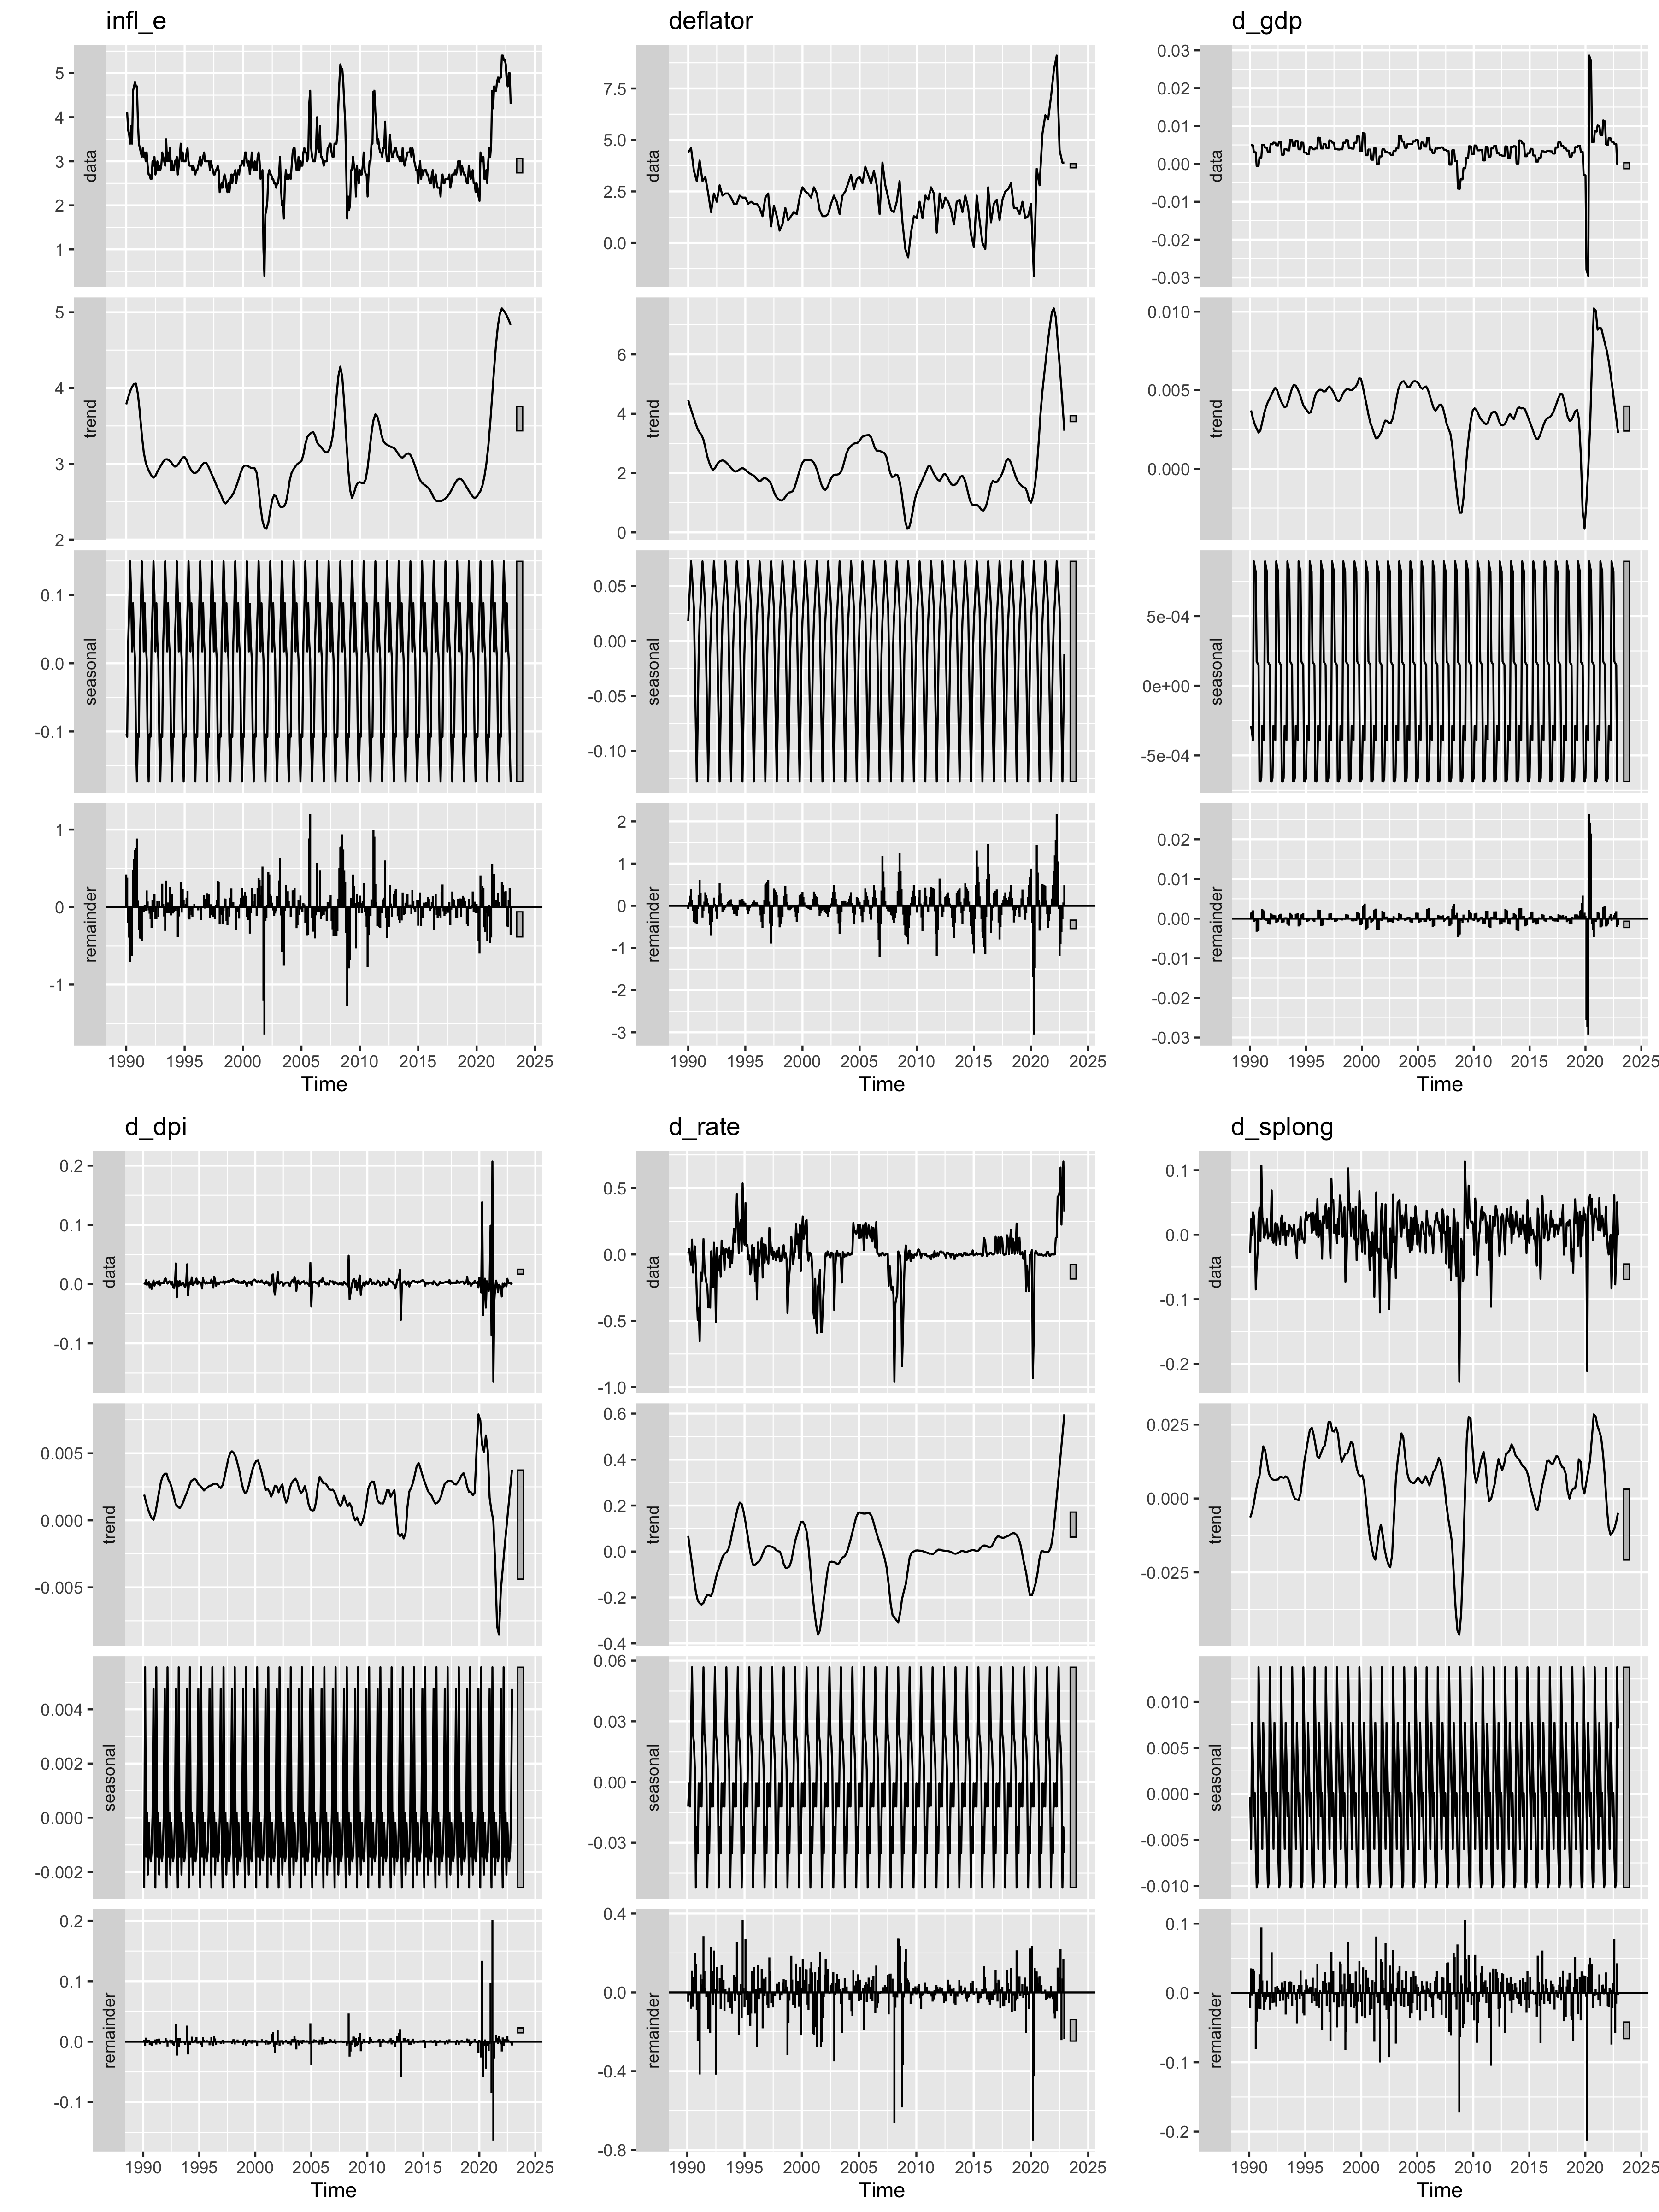
\includegraphics[width=0.95\textwidth]{IMAGES/all_decompositions.png}
    \caption{Time series decomposition of stationary series (levels and deltas)}
    \label{fig:all_decompvf}
\end{figure}

\begin{comment} #subfigures with decompositions
\begin{figure}[h!]
    \centering
    \begin{subfigure}[b]{0.7\textwidth}
        \centering
        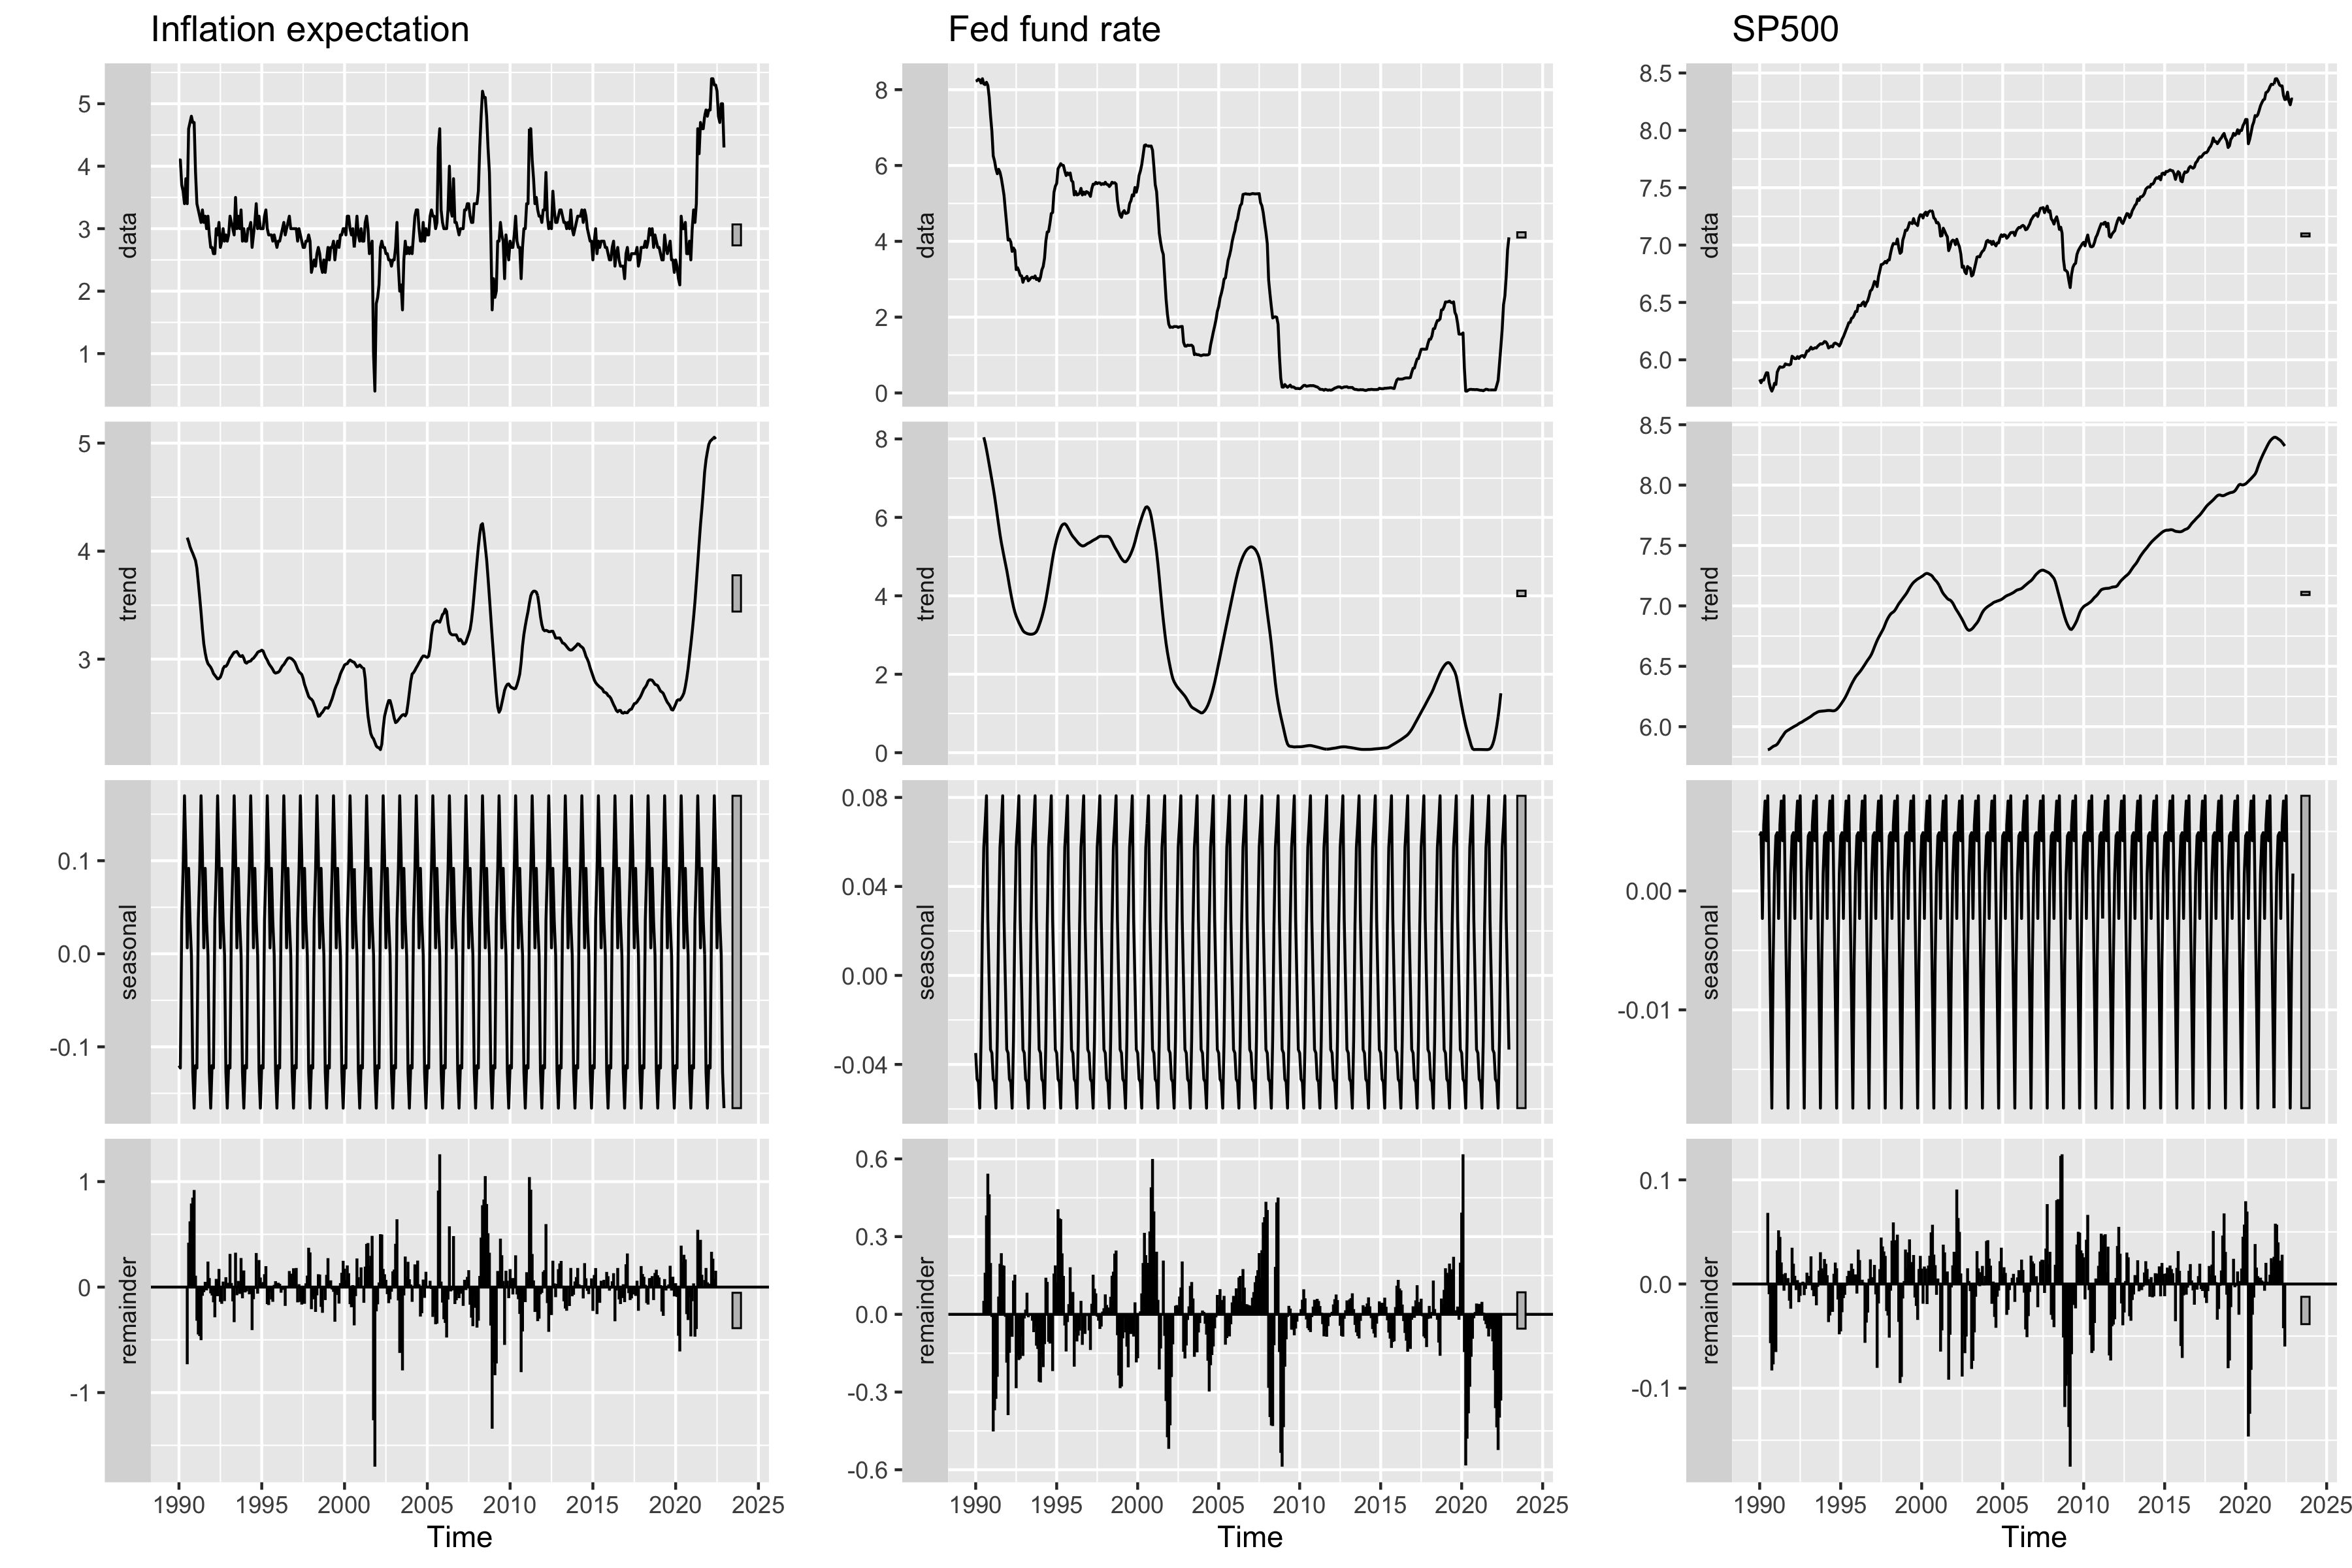
\includegraphics[width=\textwidth]{IMAGES/decomposition_i.png}
        \caption*{}
    \end{subfigure}
    \hfill
    \begin{subfigure}[b]{0.7\textwidth}
        \centering
        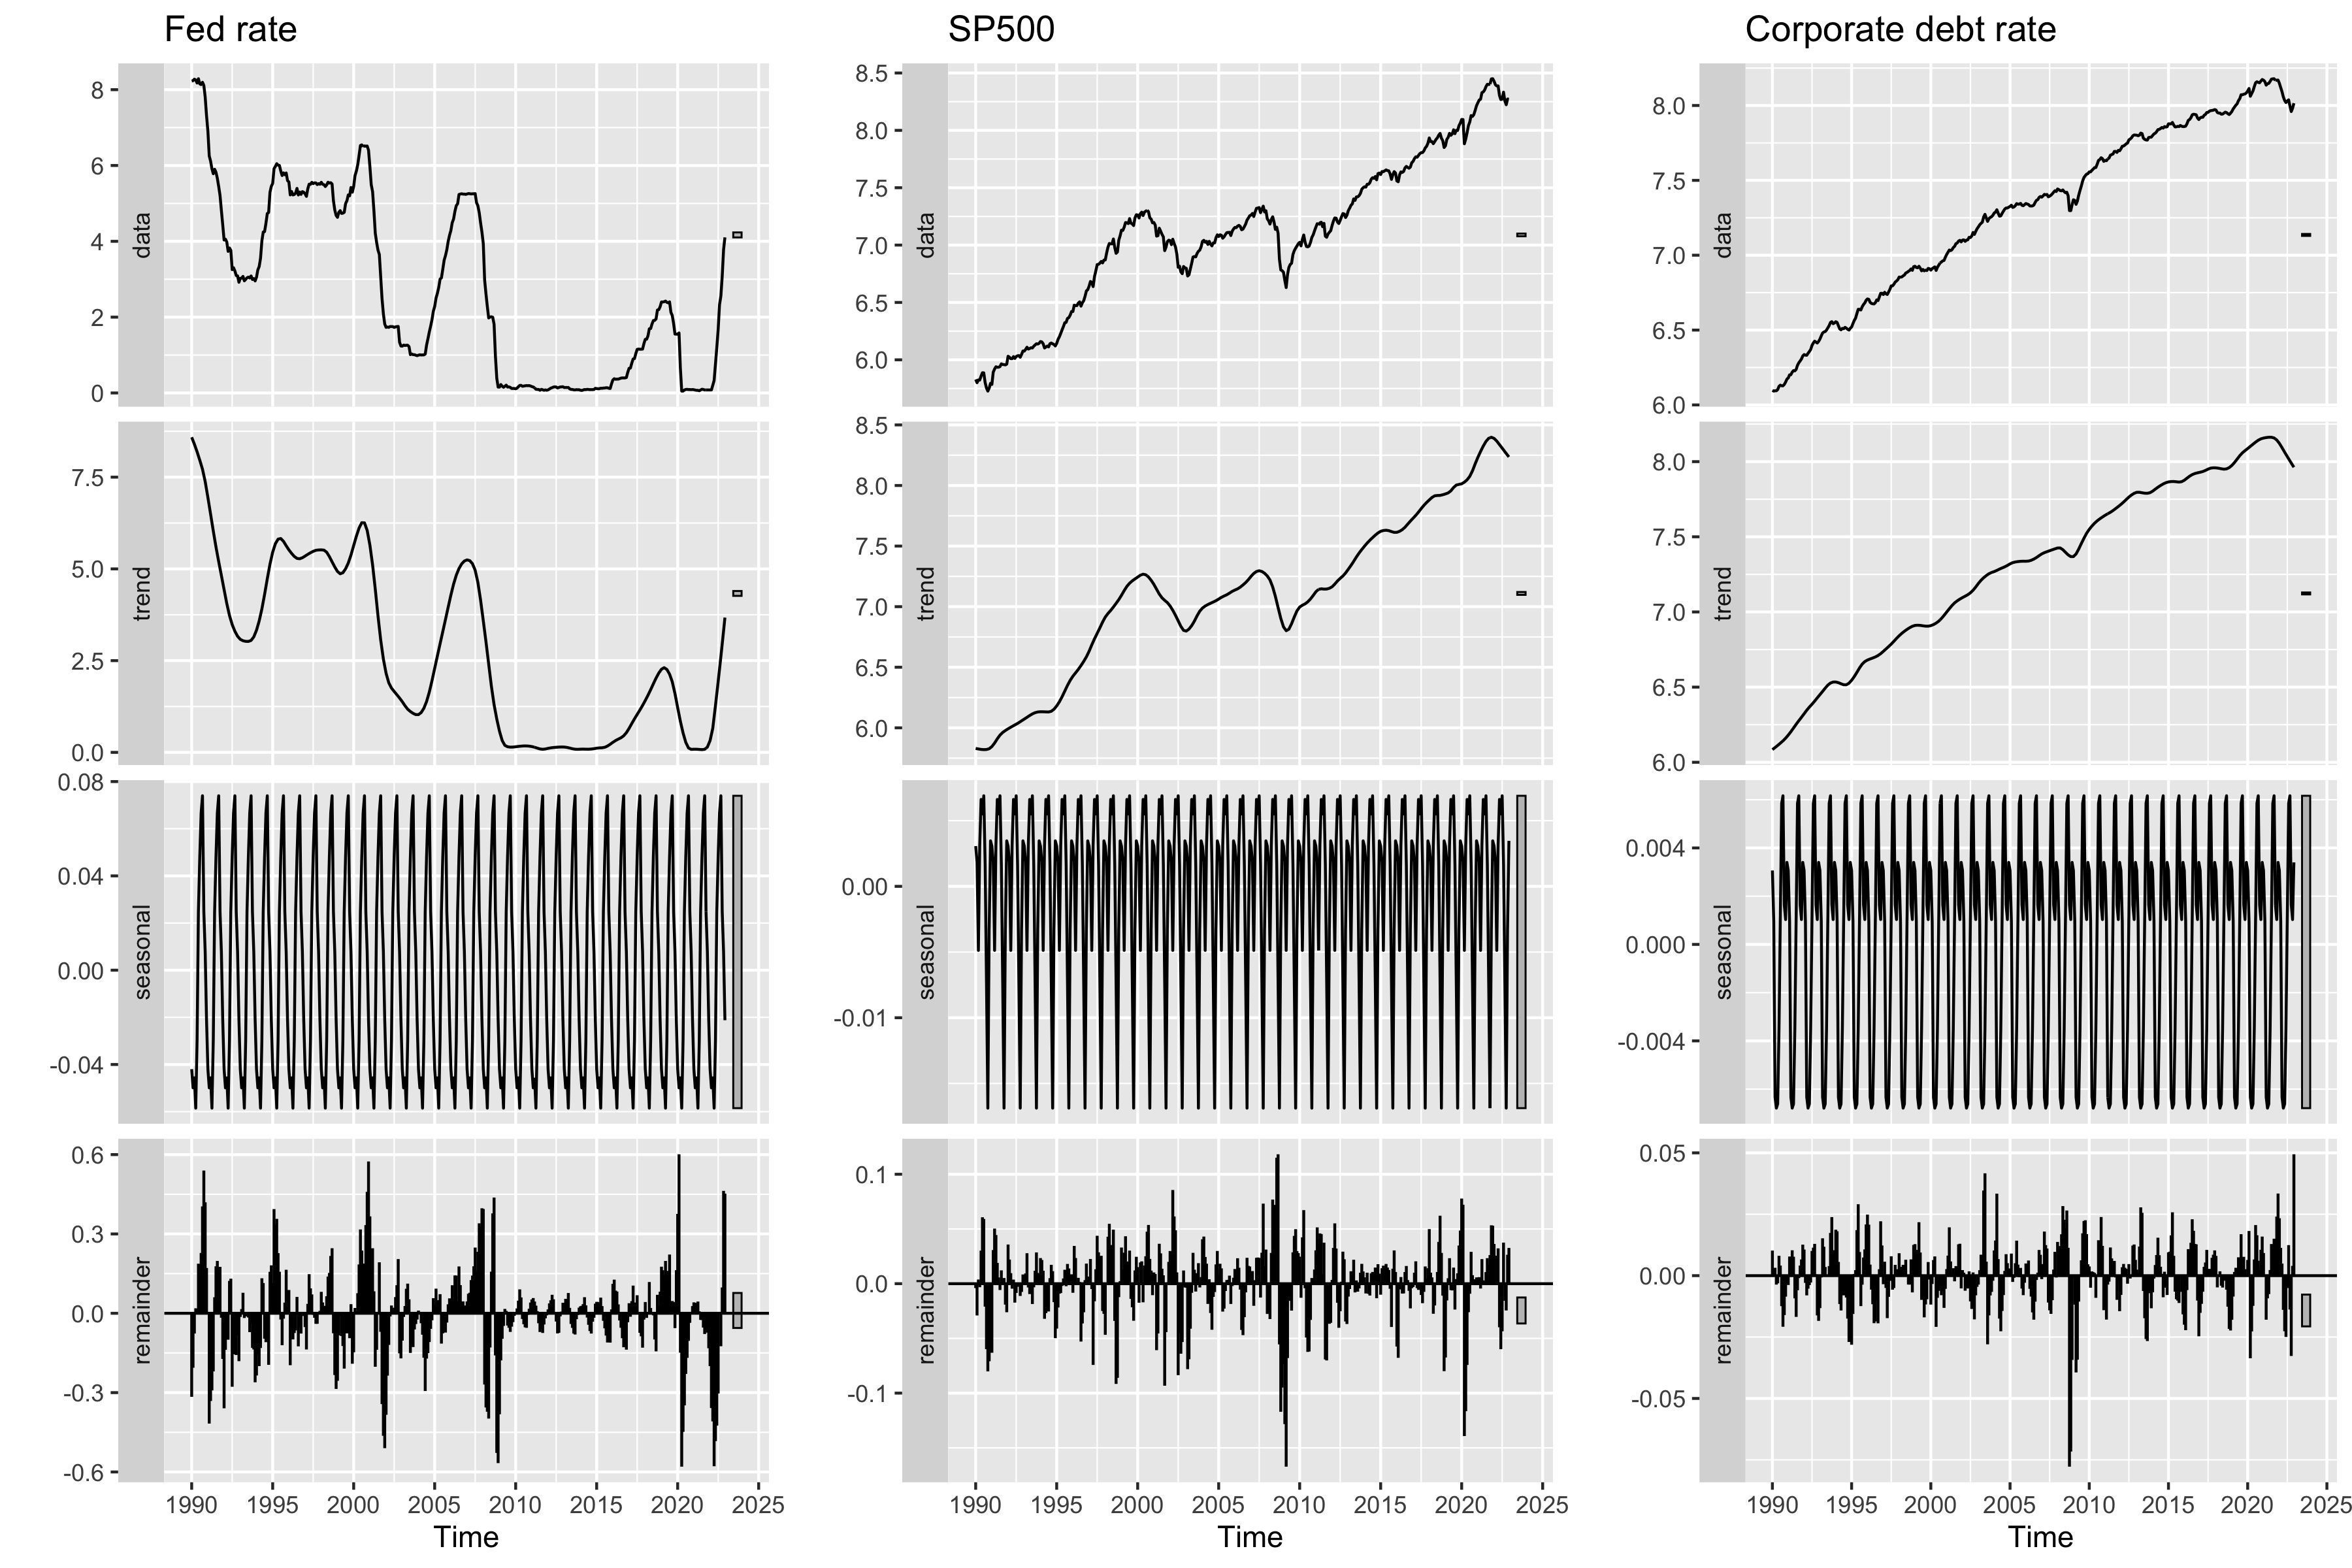
\includegraphics[width=\textwidth]{IMAGES/decomposition_ii.png}
        \caption*{}
    \end{subfigure}
    \hfill 
    \caption{Time series decomposition}
    \label{fig:decomposition}
\end{figure}
\end{comment}

    \subsubsection{Estimation of the parameters in the stationary series}

We perform we estimate the following regression to test the significance of the deterministic trend, drift and seasonal components:
    \begin{equation*}
        X_t = \alpha + \beta \times t + \sum_{i=1}^{11} \rho_i \1_{\text{month}=i} +c_t
    \end{equation*}

The results of this estimation are found in Table \ref{tab:ols_dec_levels} for the series that are I(0) in levels, and in Table \ref{tab:ols_dec_deltas} for the series of first differences of the series that were not stationary 

The coefficients on trend correspond to $\hat{\beta}$, those on the variables starting with M are $\hat{\rho_i}$. 
Since there is a monthly dummy less than the number of months, the coefficient on Contsnat encompasses both $\alpha$ and the coefficient on the last month. 
We tried to change the dummy that is ommitted and it does not change the results in terms of significance. 


\input{TABLES/ols_decomp_levels}
\input{TABLES/ols_decomp_deltas}

\begin{comment}
{Seasonality} \label{sec:adf}

From the decompositions made in the previous section, in Figure \ref{fig:decomposition} we can see that R picks up small seasonal variations in each series (the values on the y-axis are rather very small). 
The estimations of the seasonal coefficients are reported in Table \ref{tab:seasons}, which indeed shows very small coefficients.
We nonetheless decided to work with deseasonalized series even if the changes are minimal.


% Table created by stargazer v.5.2.3 by Marek Hlavac, Social Policy Institute. E-mail: marek.hlavac at gmail.com
% Date and time: Tue, Dec 05, 2023 - 20:24:19
\begin{table}[!htbp] \centering 
  \caption{Estimation of the seasonality of each series} 
  \label{tab:seasons} 
\begin{tabular}{@{\extracolsep{5pt}} ccccccccccccc} 
\\[-1.8ex]\hline 
\hline \\[-1.8ex] 
 & JAN & FEB & MAR & APR & MAY & JUN & JUL & AUG & SEP & OCT & NOV & DEC \\ 
\hline \\[-1.8ex] 
infl\_e & -0.104 & -0.108 & 0.031 & 0.078 & 0.149 & 0.1 & 0.017 & 0.088 & 0.031 & 0.006 & -0.116 & -0.173 \\ 
deflator & 0.018 & 0.035 & 0.053 & 0.072 & 0.06 & 0.045 & 0.03 & -0.024 & -0.078 & -0.128 & -0.072 & -0.012 \\ 
unempl & 0.464 & 0.327 & 0.132 & -0.045 & -0.074 & 0.296 & 0.284 & 0.007 & -0.257 & -0.406 & -0.379 & -0.349 \\ 
rate & -0.042 & -0.05 & -0.046 & -0.059 & -0.03 & 0.025 & 0.048 & 0.067 & 0.074 & 0.025 & 0.008 & -0.021 \\ 
splong & 0.003 & 0.002 & -0.005 & 0.003 & 0.007 & 0.006 & 0.007 & 0.002 & -0.007 & -0.017 & -0.003 & 0.003 \\ 
corp\_debt & 0.003 & 0.001 & -0.006 & -0.007 & -0.007 & -0.004 & 0.001 & 0.006 & 0.006 & 0.002 & 0.001 & 0.003 \\ 
\hline \\[-1.8ex] 
\end{tabular} 
\end{table} 

\end{comment}



    \subsection{Cyclical component}

To assess the behavior of the cyclical component, we detrend the series, substract the coefficient of the constant and remove the seasonal component when the coefficients are significant. After extracting these components, we would like to model them with appropiate $ARMA(p,q)$ models.

To do so, we first produce PACF (Figure \ref{fig:pacf_all}) and ACF graphs (Figure \ref{fig:acf_all}) to know respectively the maximum values that $p$ and $q$ could take, $\bar{p}, \bar{q}$.
The blue dotted lines onthe figures are the 95\% confidence intervals.
$\bar{p}, \bar{q}$ are given by the last period where the PACF or the ACF are significantly different from zero. 
We were surprised by the rather long memory of some of the processes, notably of the inflation expectation, the GDP deflator, and the first difference of the Fed fund rate series but we double checked and the series are stationary. 

\begin{figure}[h!]
    \centering
    \begin{subfigure}[b]{0.45\textwidth}
        \centering
        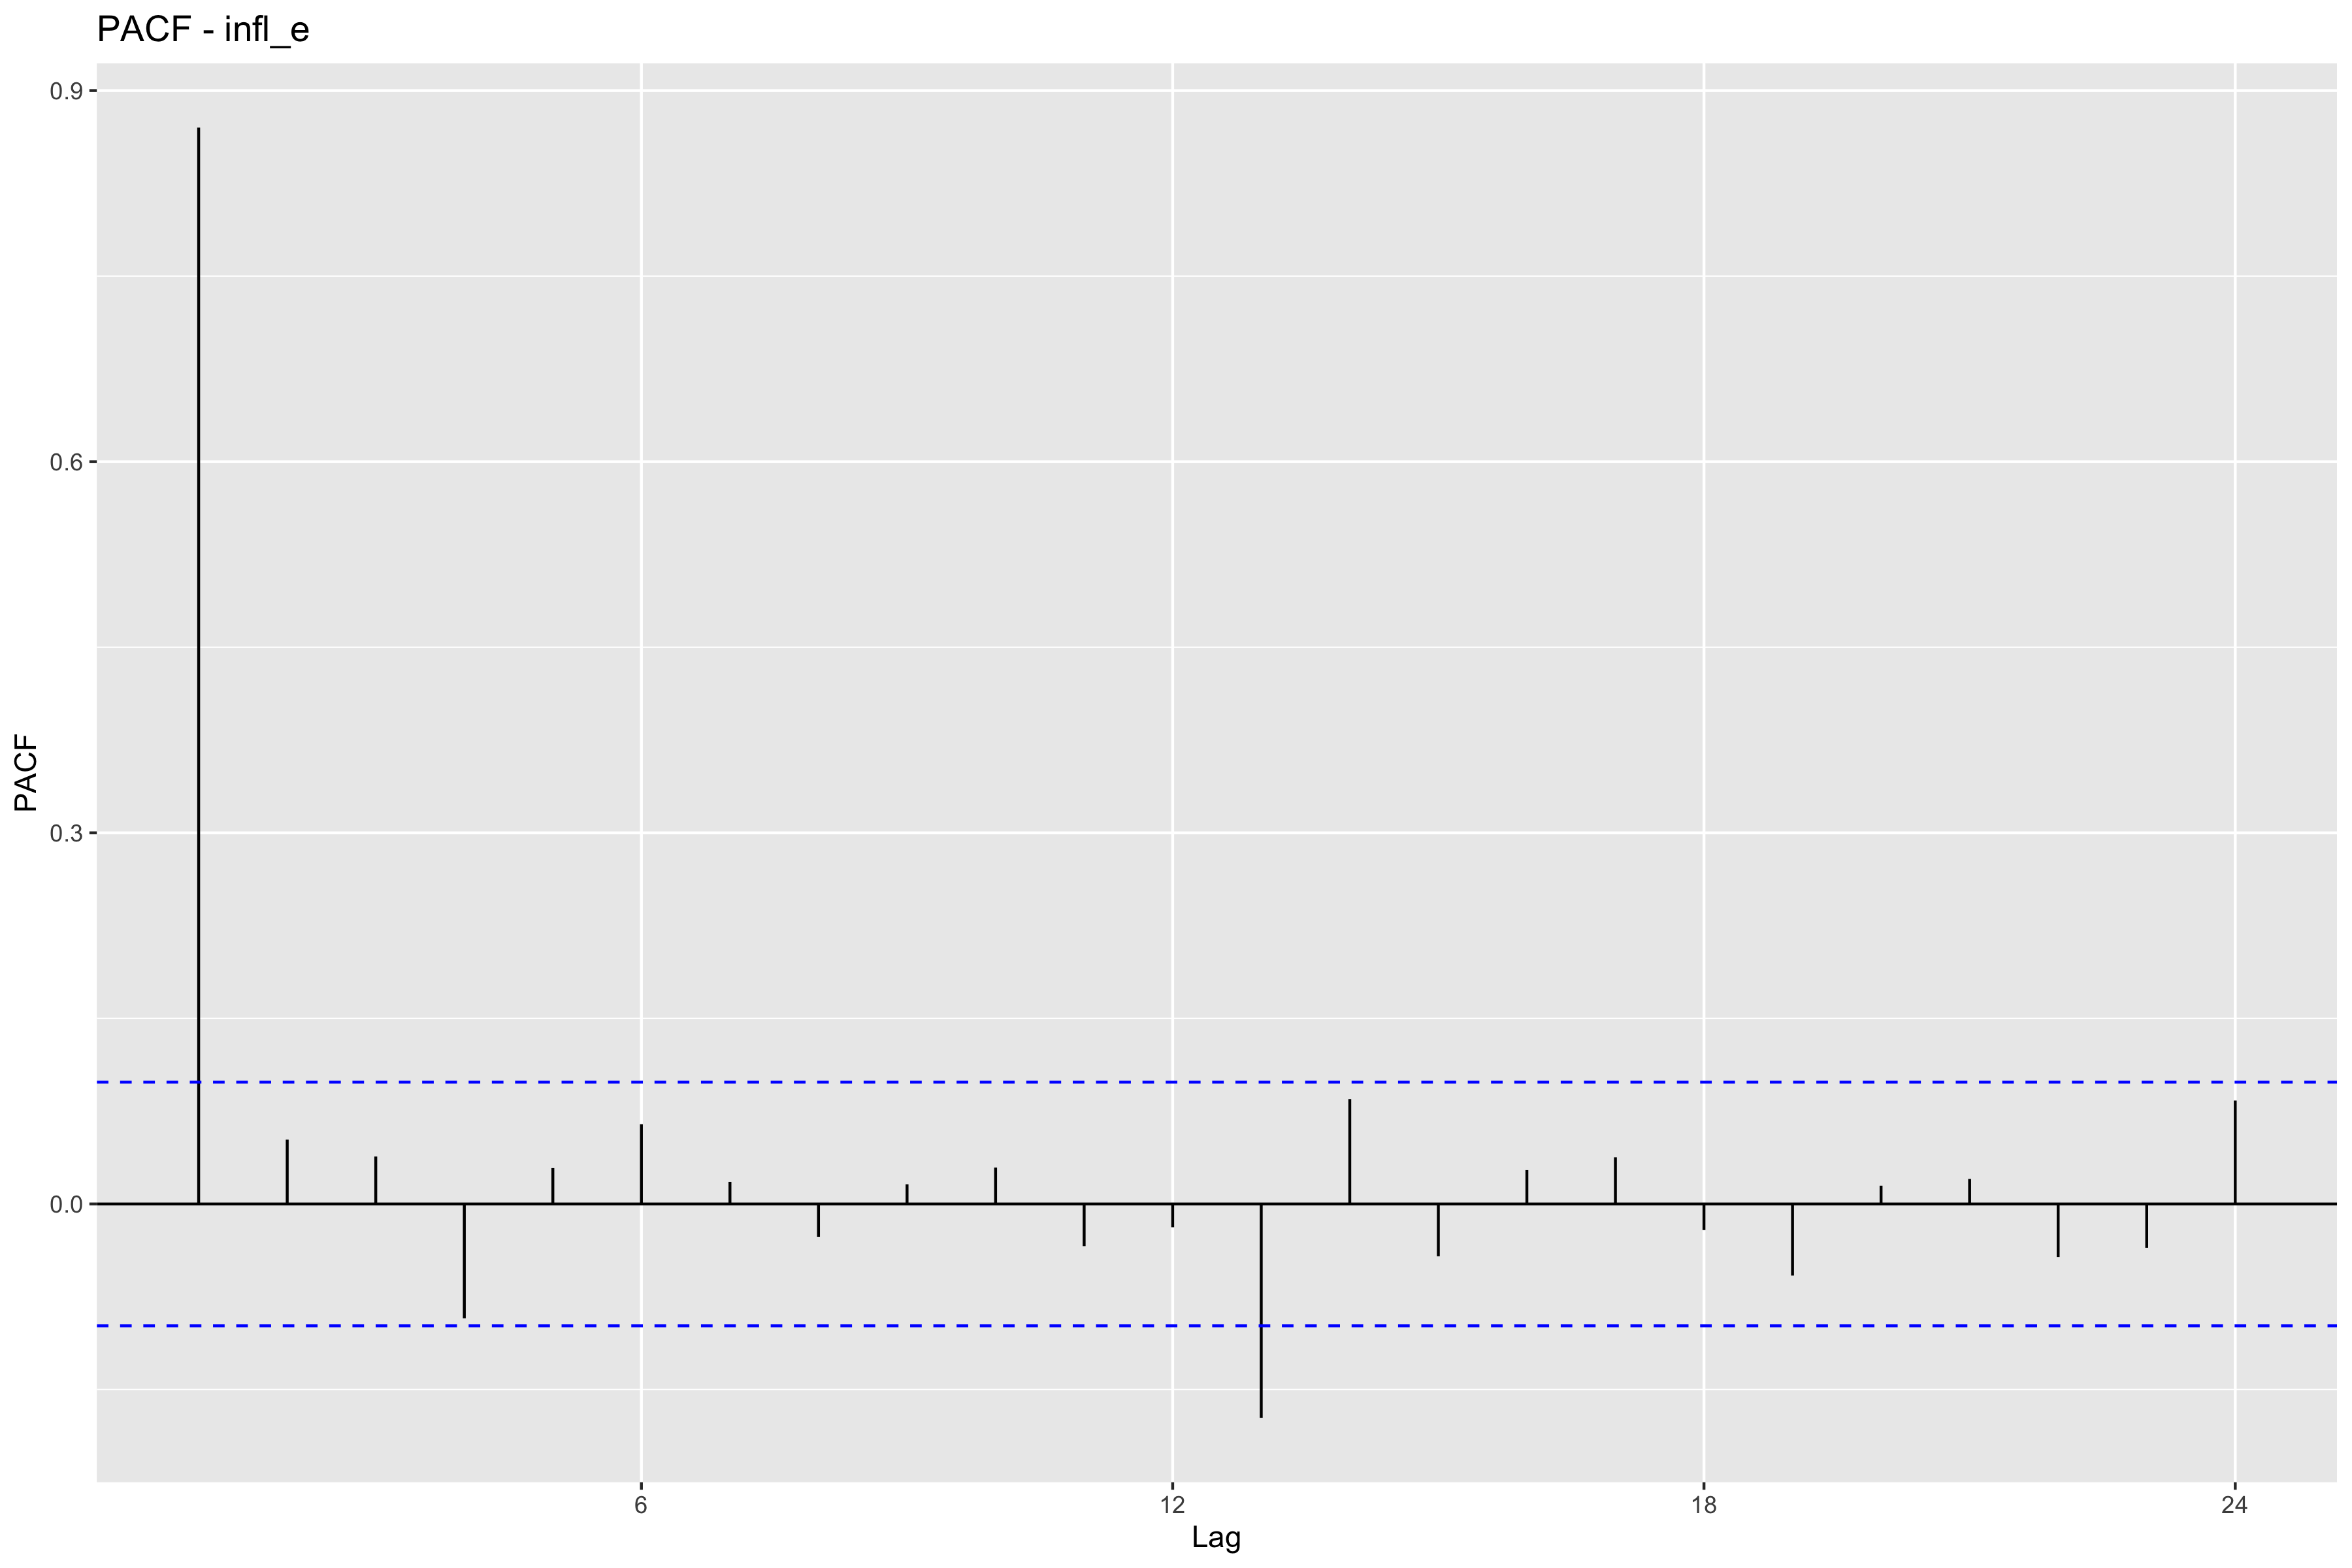
\includegraphics[width=\textwidth]{IMAGES/pacf_infl.png}
        \caption*{Inflation expectation}
    \end{subfigure}
    \hfill
    \begin{subfigure}[b]{0.45\textwidth}
        \centering
        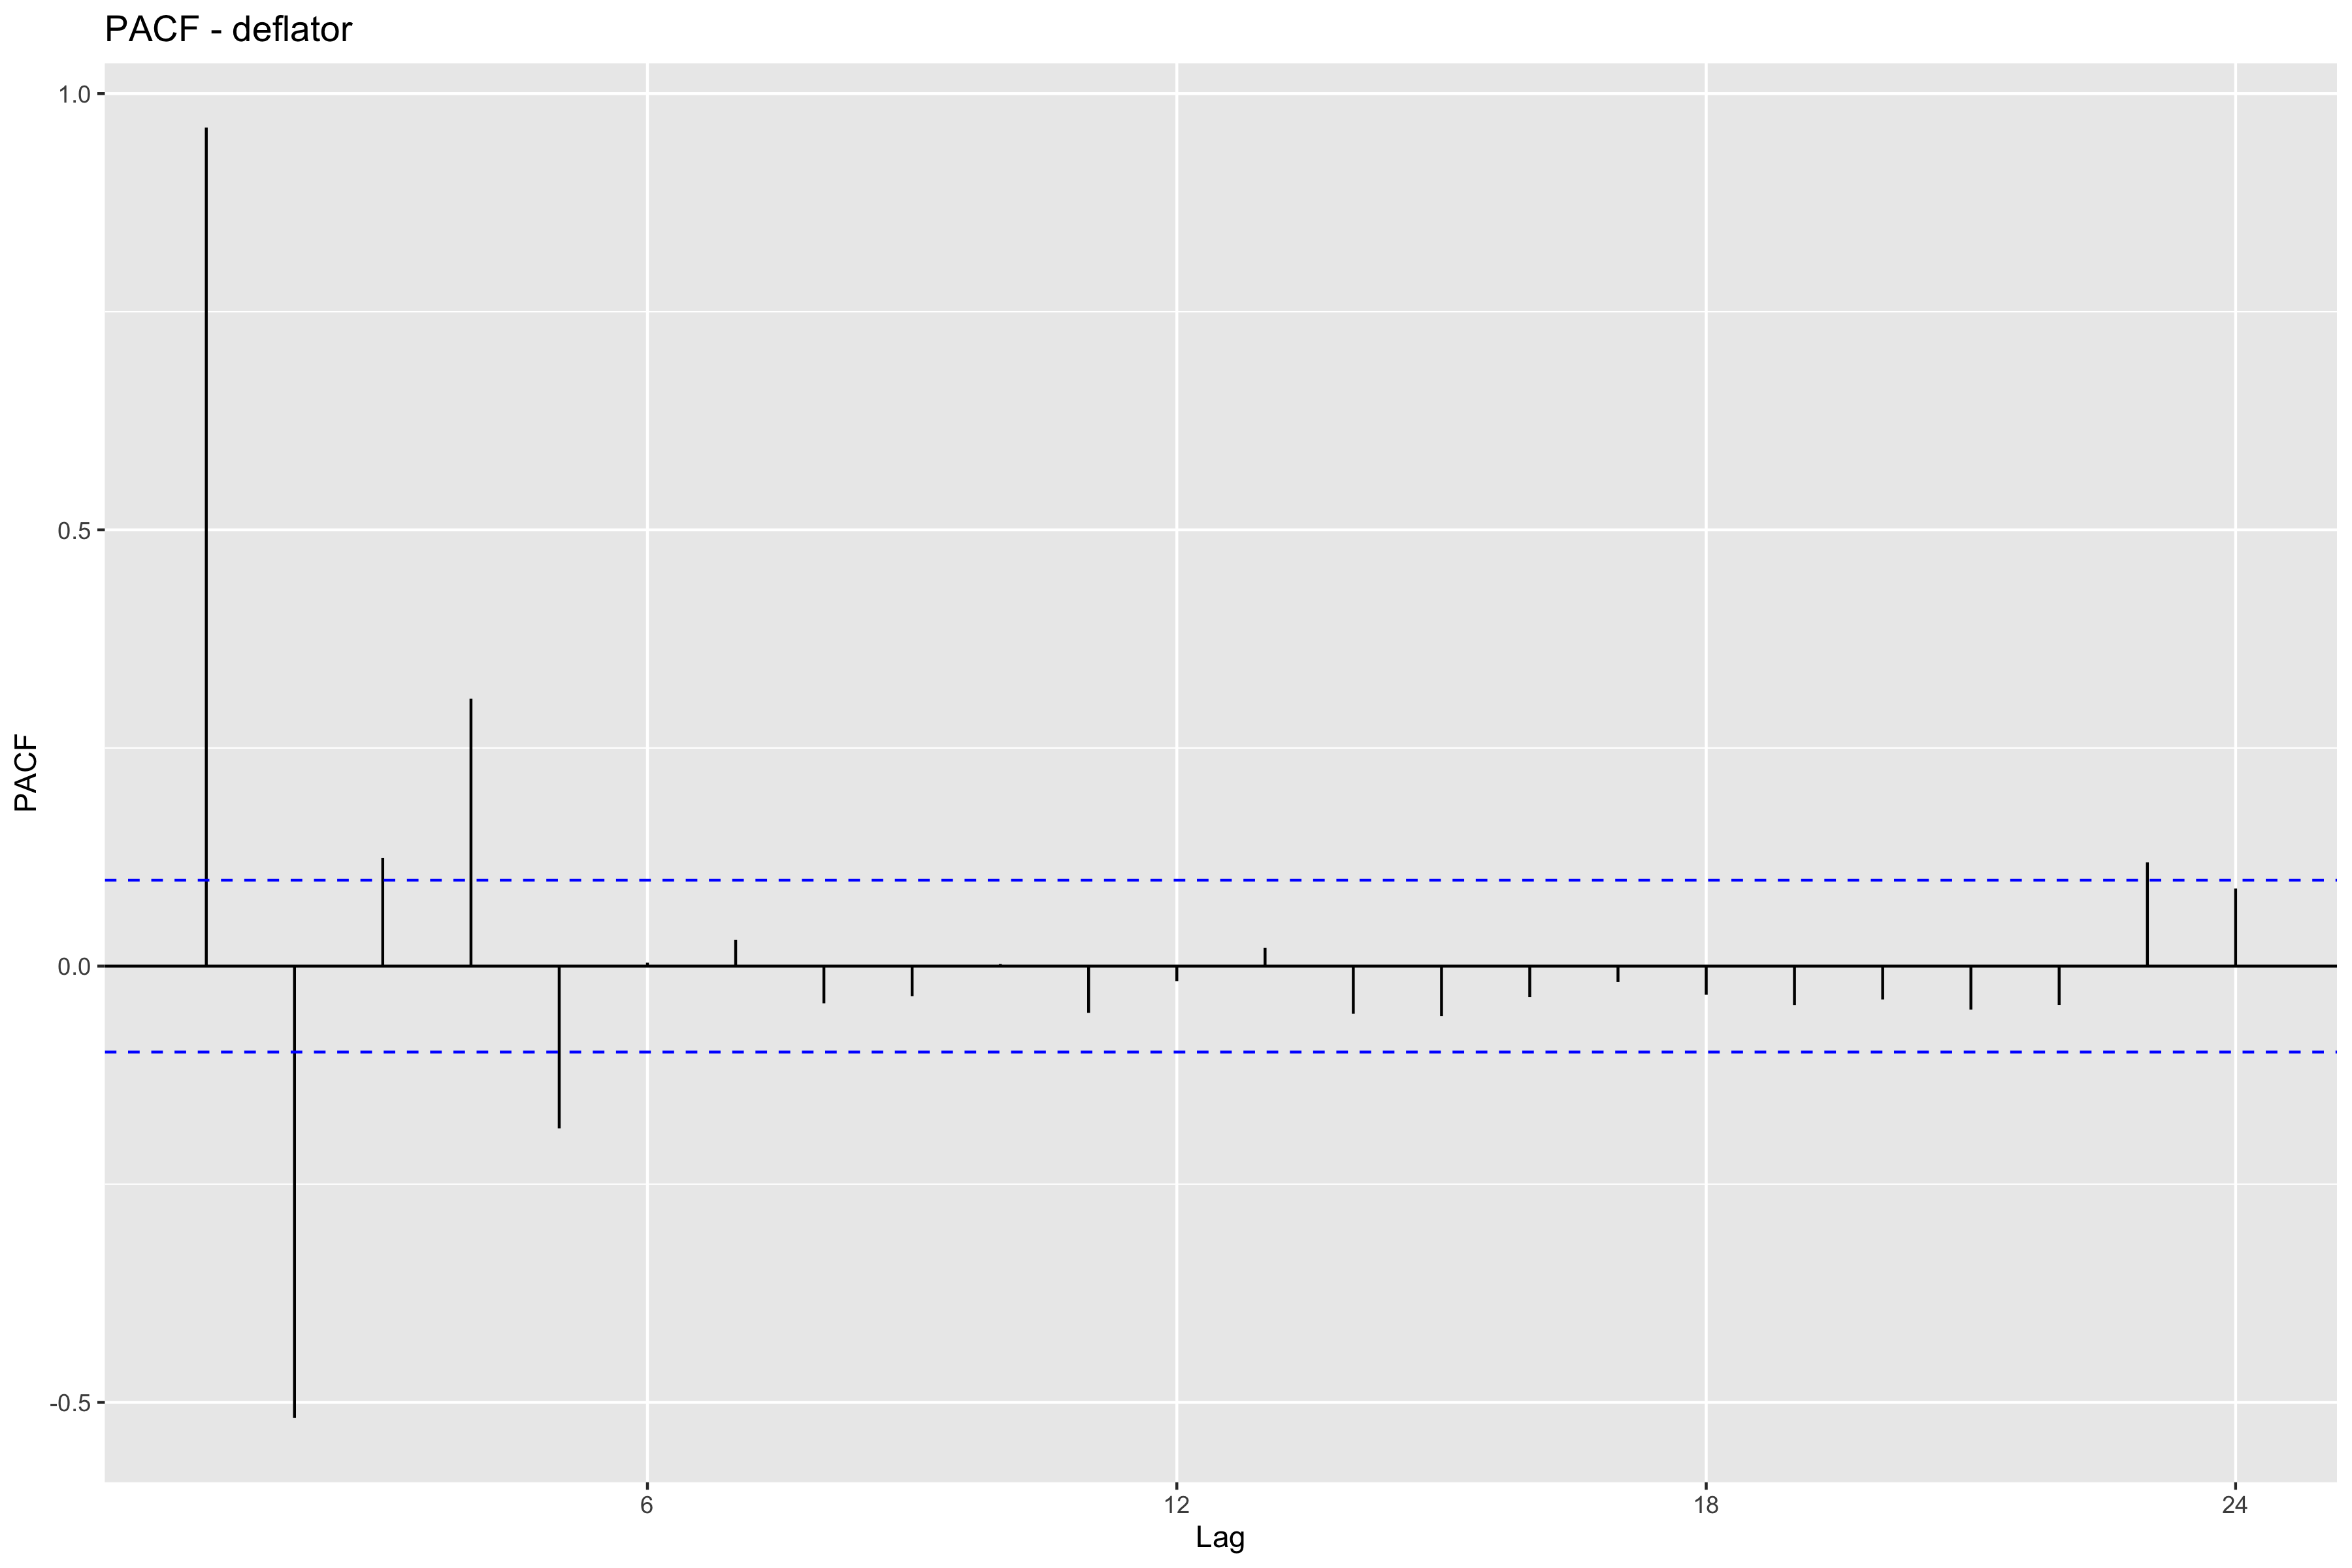
\includegraphics[width=\textwidth]{IMAGES/pacf_defl.png}
        \caption*{GDP deflator}
    \end{subfigure}
    \hfill 
    \centering
    \begin{subfigure}[b]{0.45\textwidth}
        \centering
        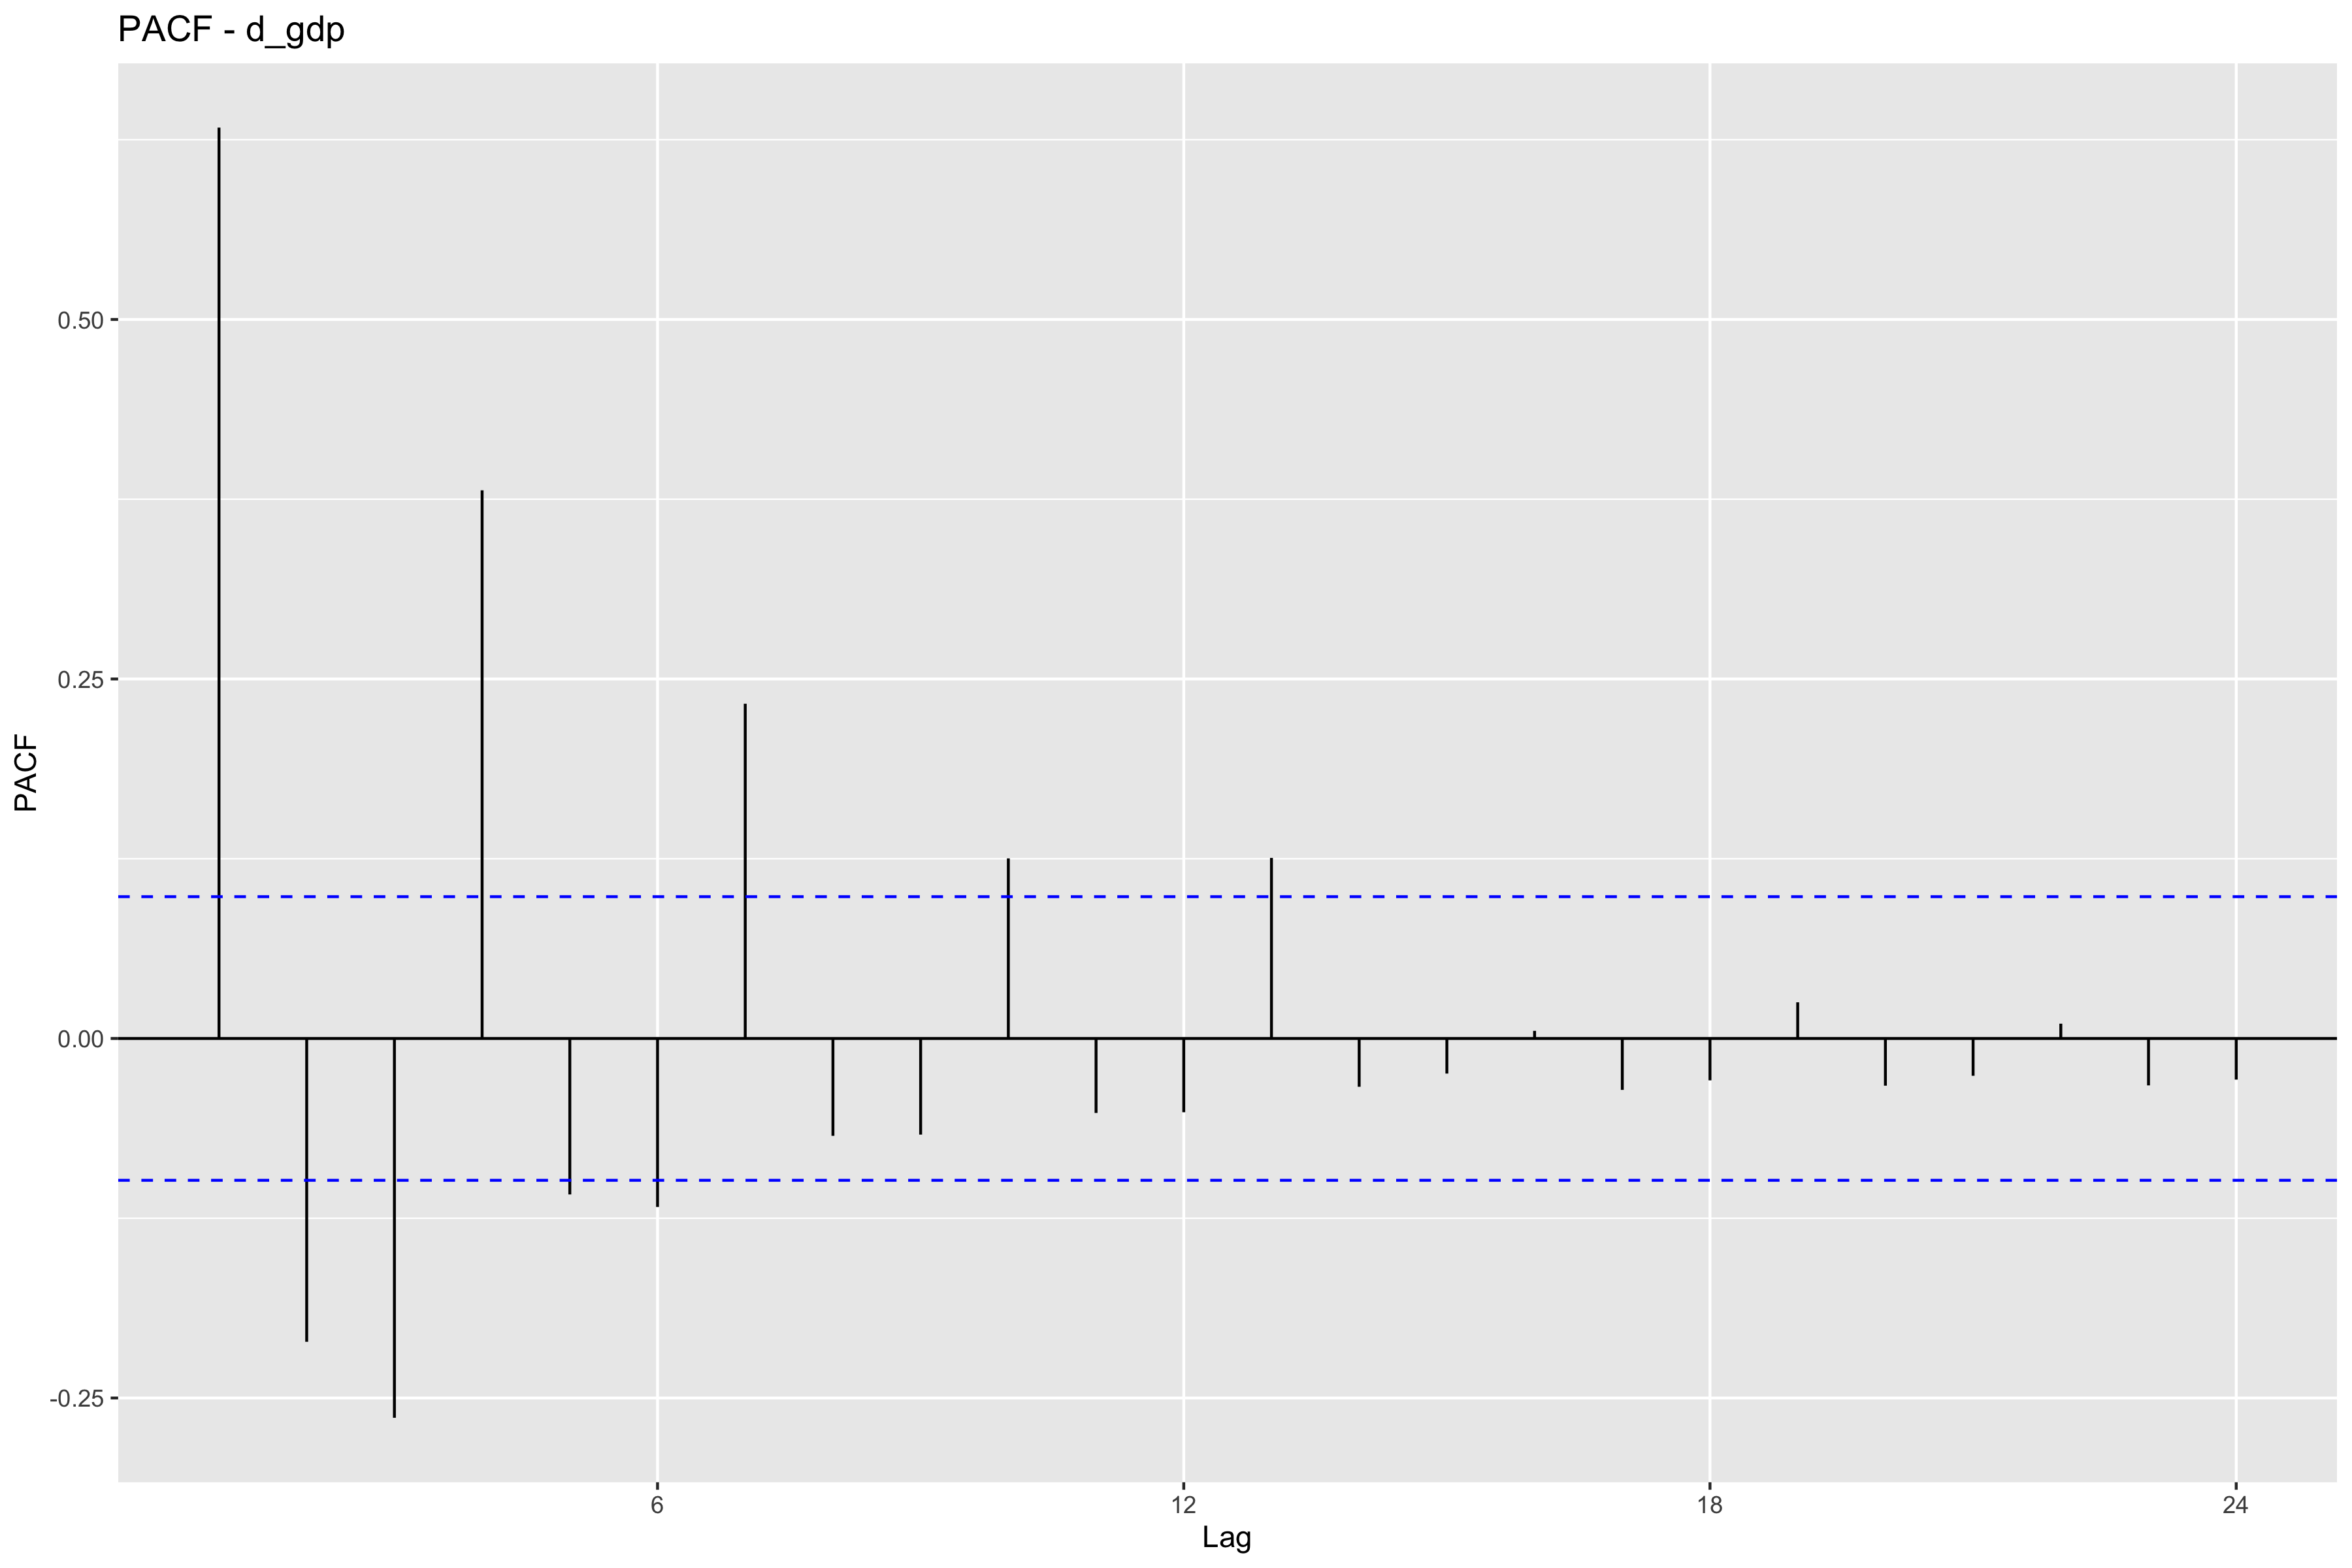
\includegraphics[width=\textwidth]{IMAGES/pacf_gdp.png}
        \caption*{GDP growth rate}
    \end{subfigure}
    \hfill
    \begin{subfigure}[b]{0.45\textwidth}
        \centering
        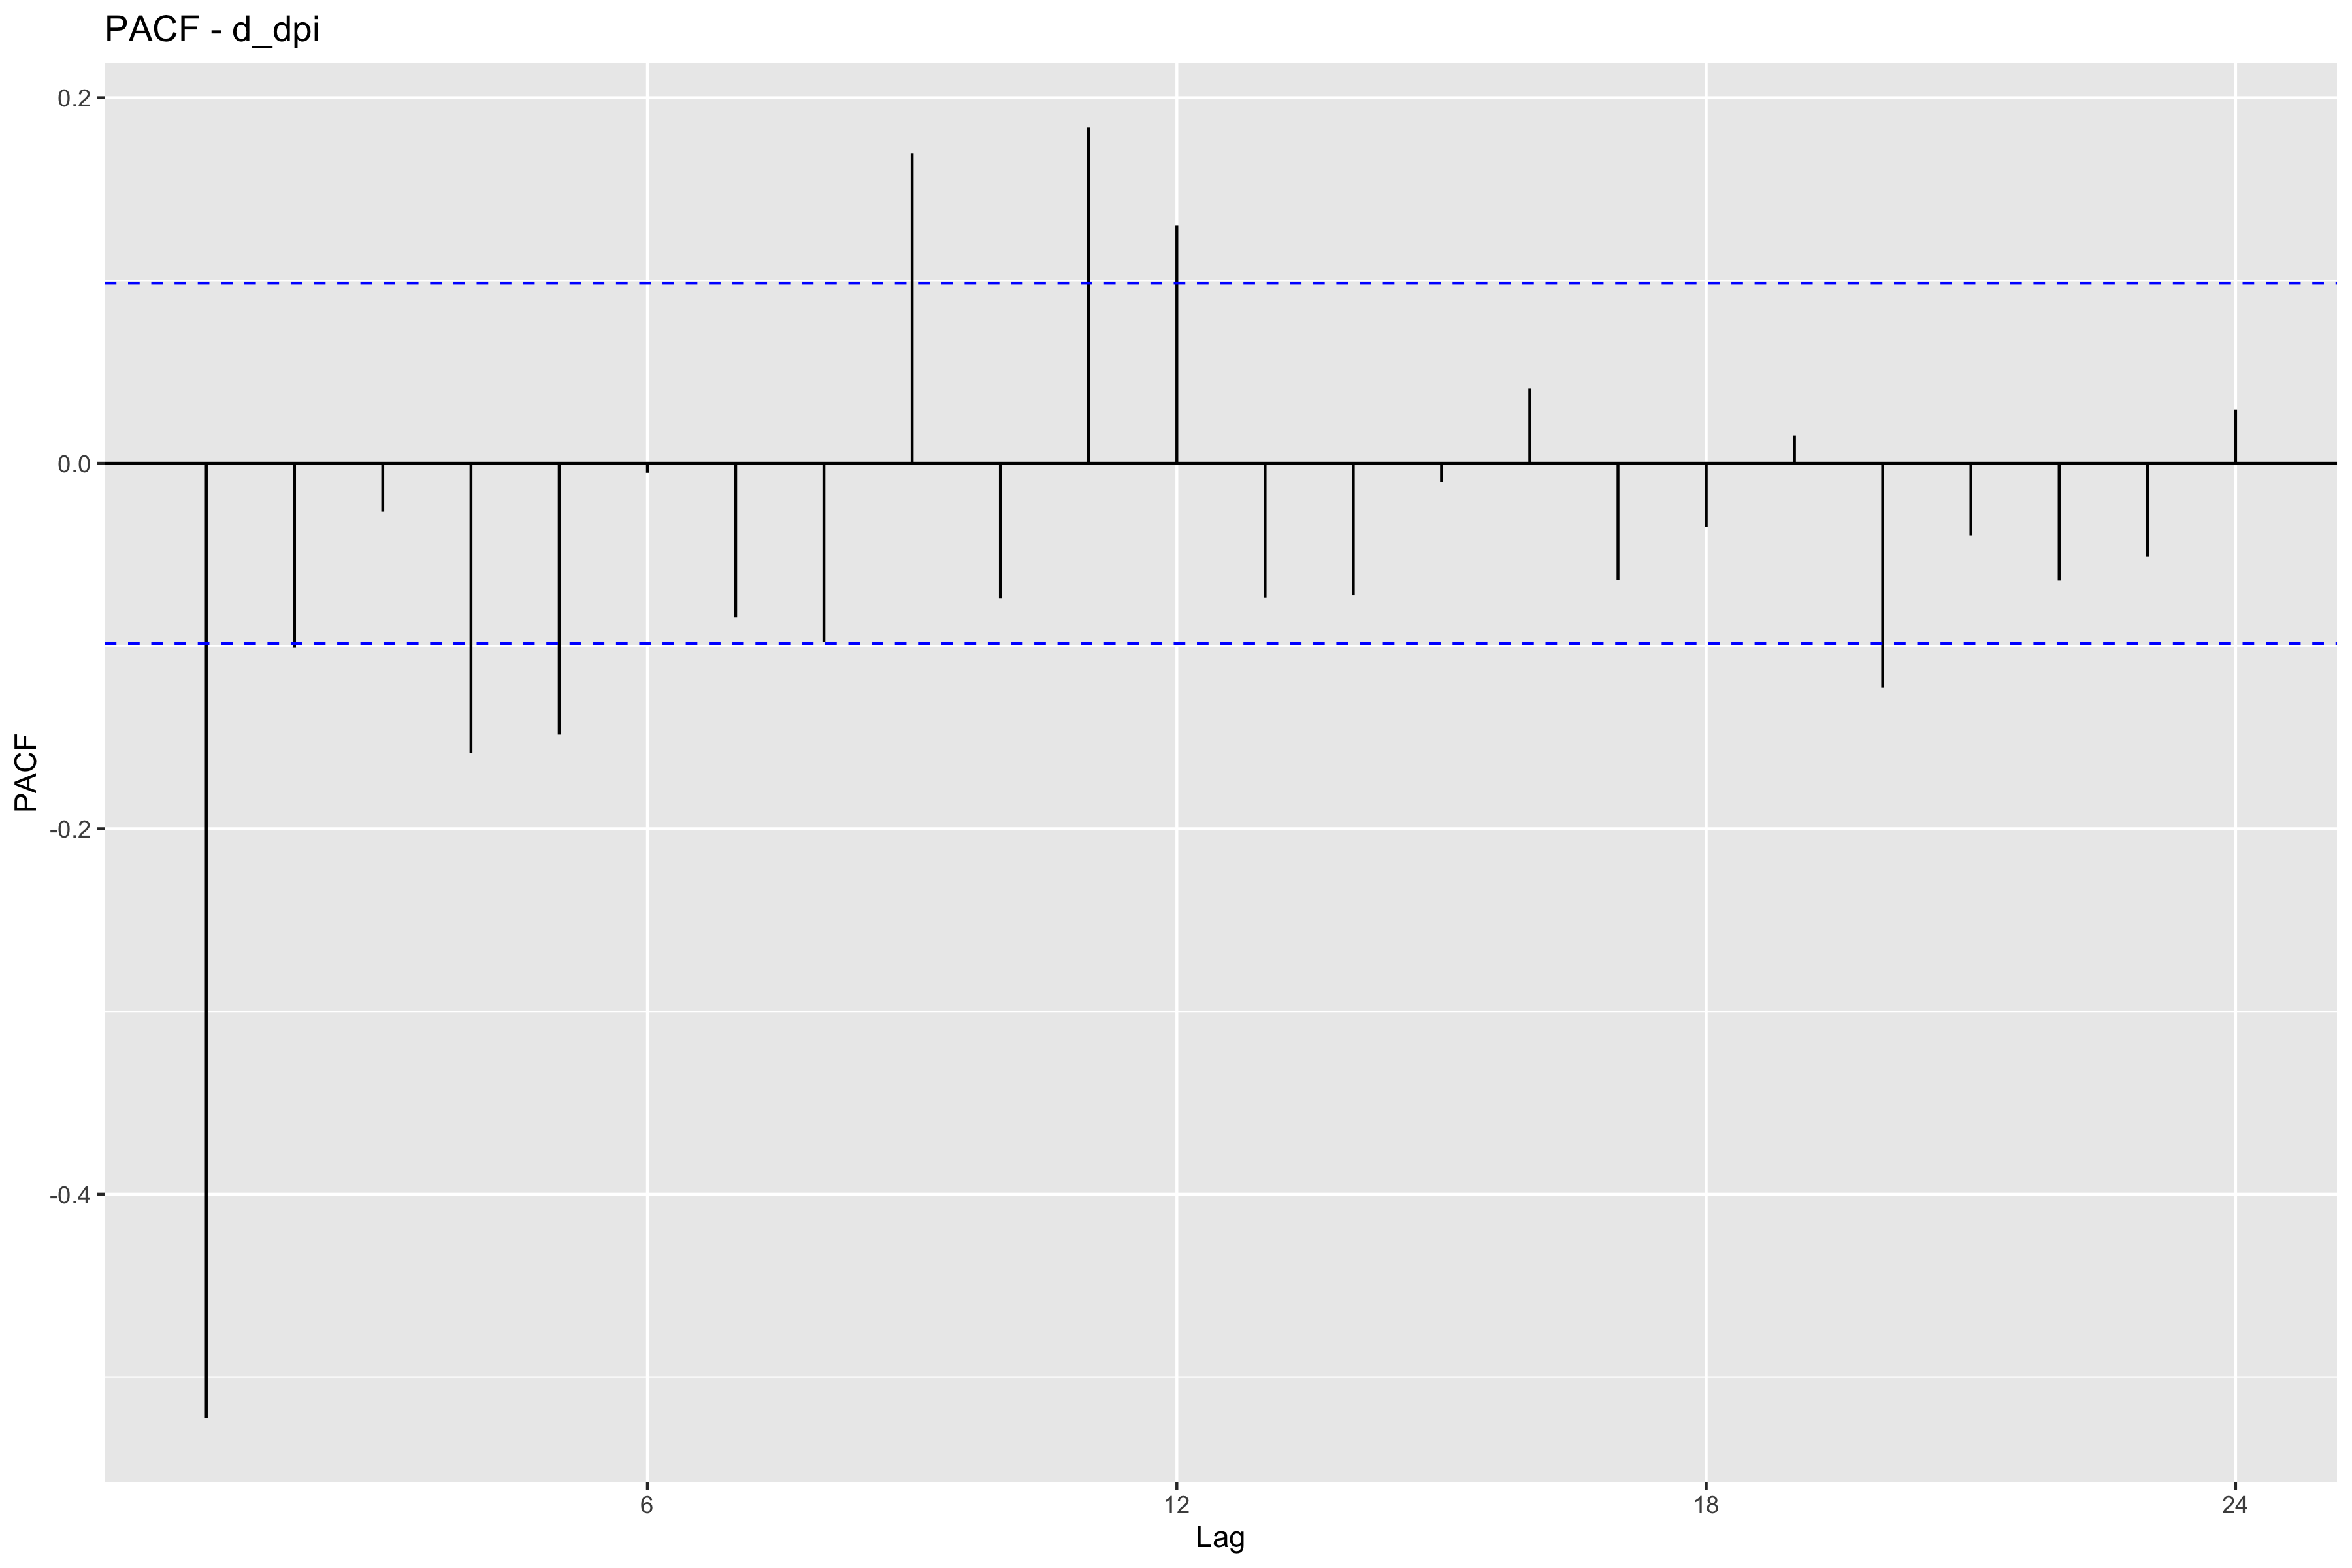
\includegraphics[width=\textwidth]{IMAGES/pacf_dpi.png}
        \caption*{Real disponsable income growth rate }
    \end{subfigure}
    \hfill 
    \centering
    \begin{subfigure}[b]{0.45\textwidth}
        \centering
        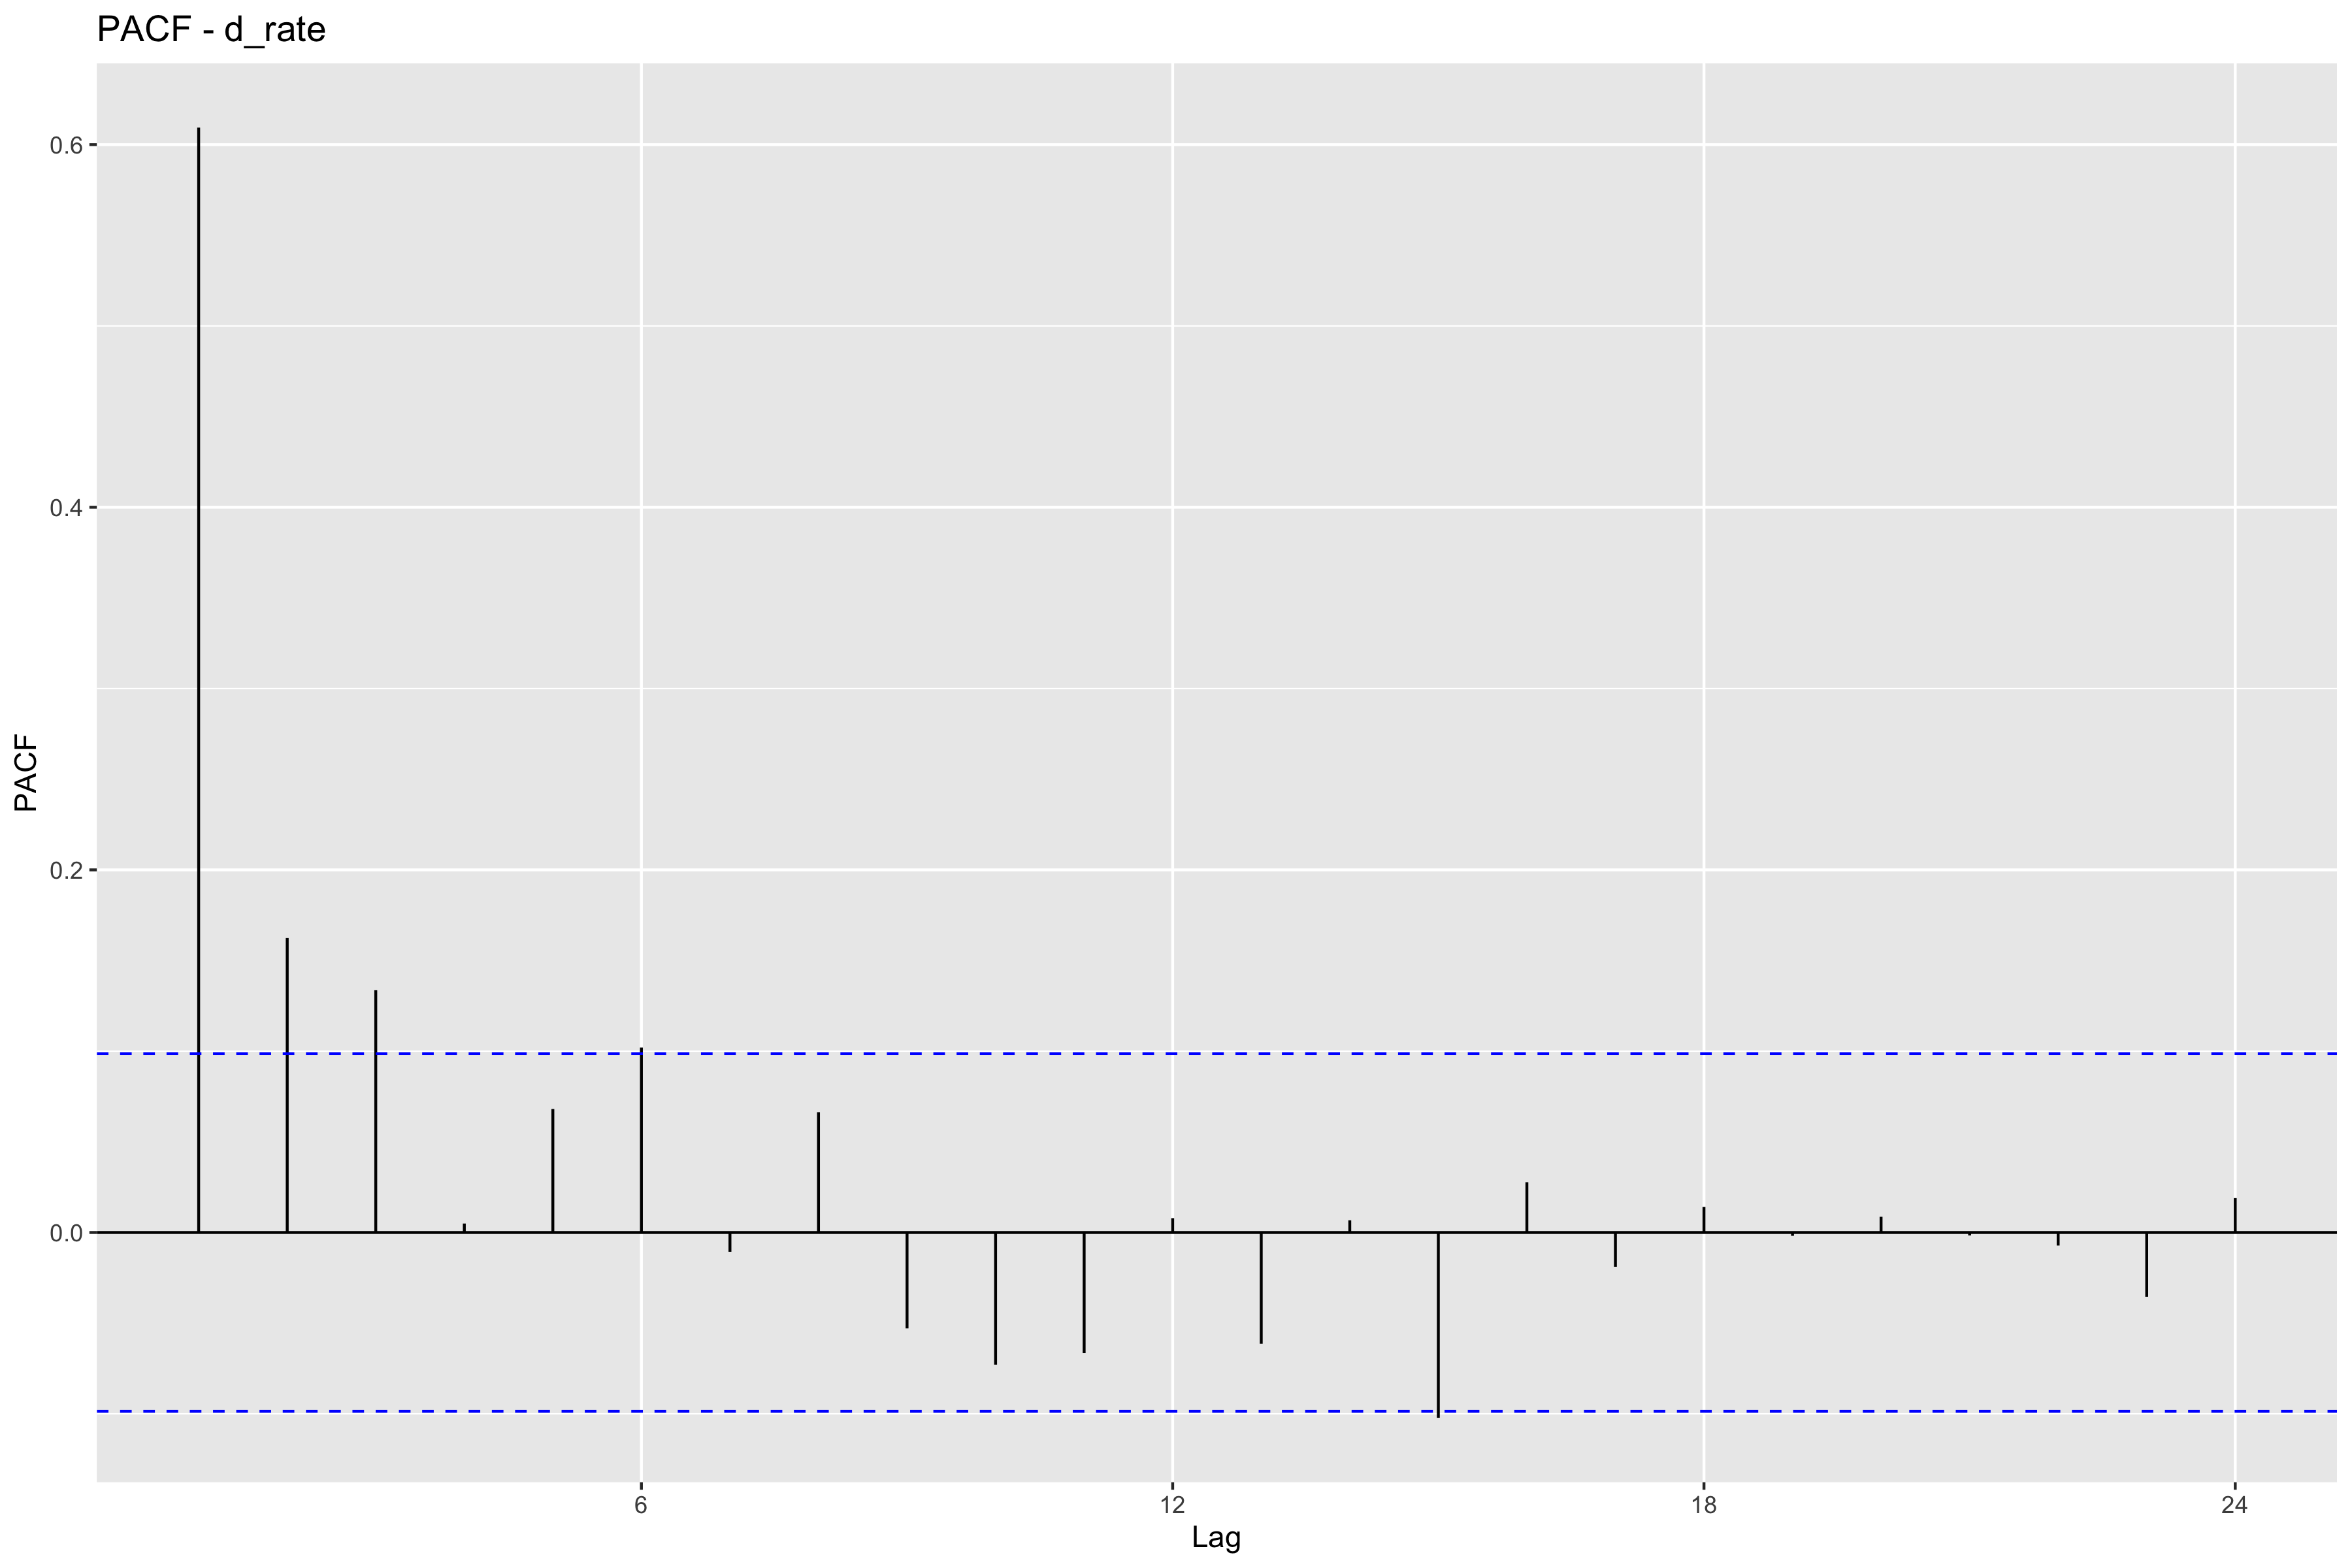
\includegraphics[width=\textwidth]{IMAGES/pacf_rate.png}
        \caption*{Fed fund rate}
    \end{subfigure}
    \hfill
    \begin{subfigure}[b]{0.45\textwidth}
        \centering
        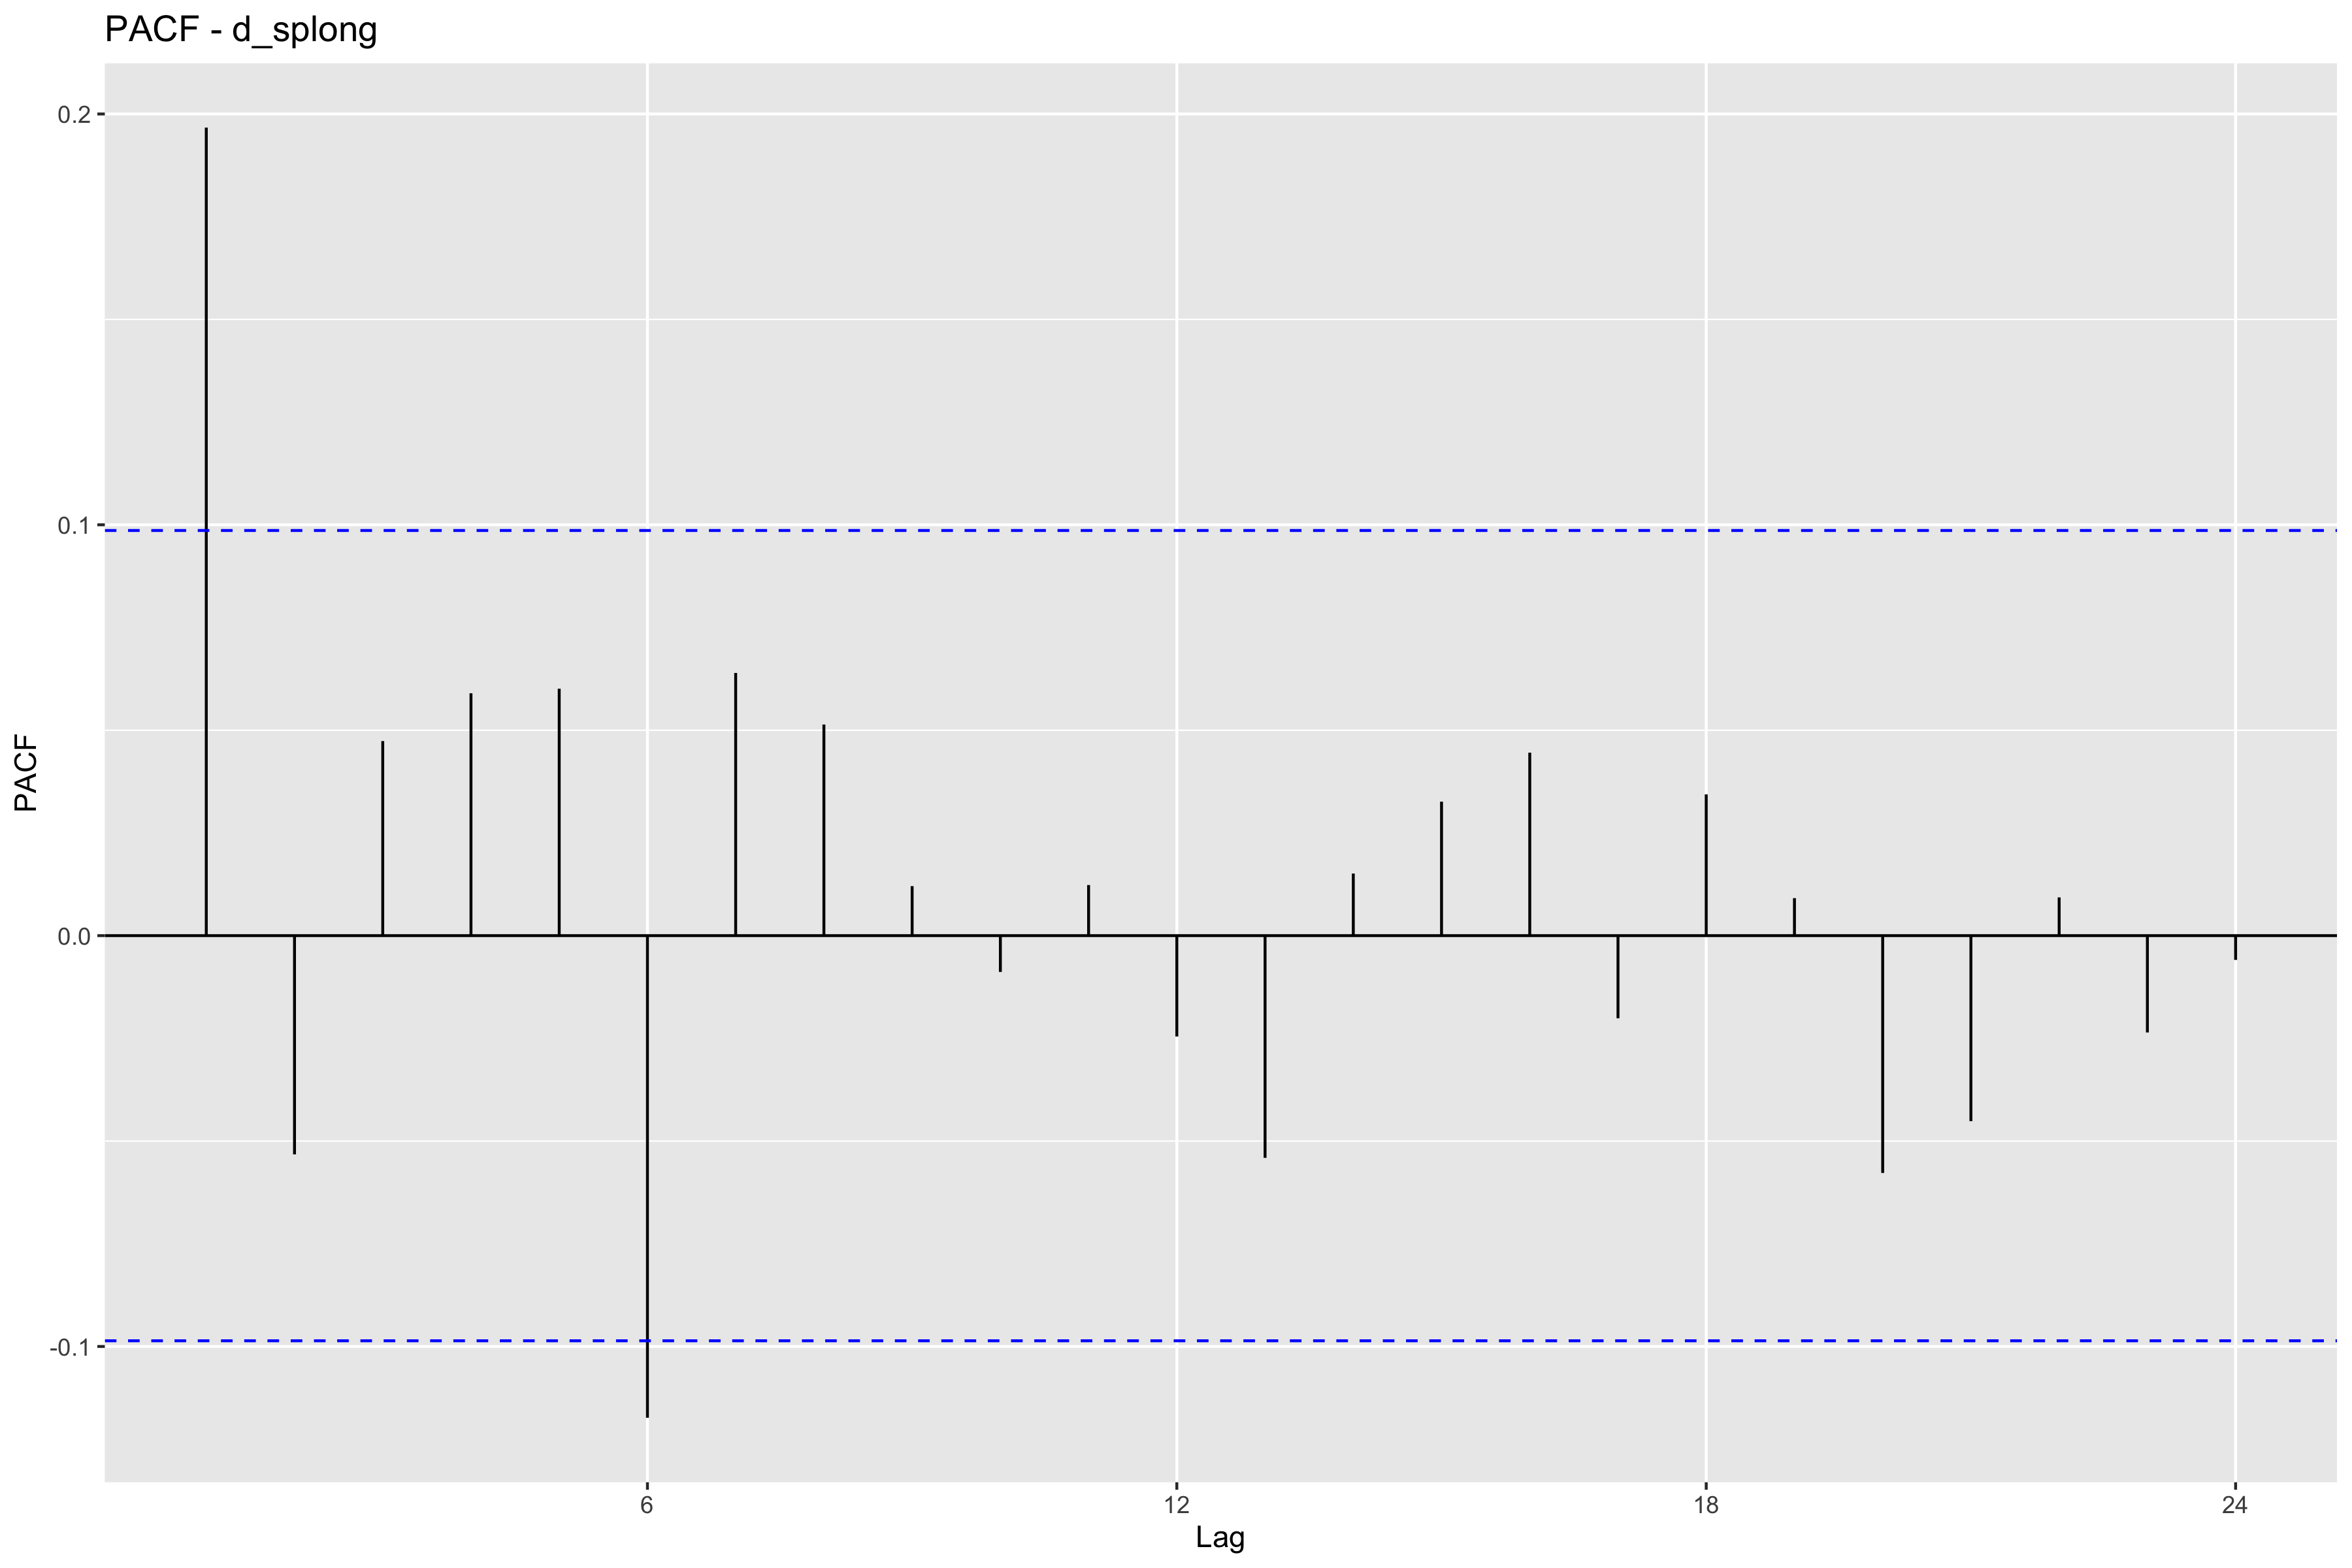
\includegraphics[width=\textwidth]{IMAGES/pacf_sp.png}
        \caption*{Returns of S\&P500}
    \end{subfigure}
    \hfill 
    \caption{PACFs}
    \label{fig:pacf_all}
    \begin{minipage}{0.9\textwidth}
        %\footnotesize
        \small{\emph{Notes}: All the series plotted are stationary: inflation expectation and GDP deflator series are in levels while the rest are first differences.}
    \end{minipage}
\end{figure}

\begin{figure}[h!]
    \centering
    \begin{subfigure}[b]{0.45\textwidth}
        \centering
        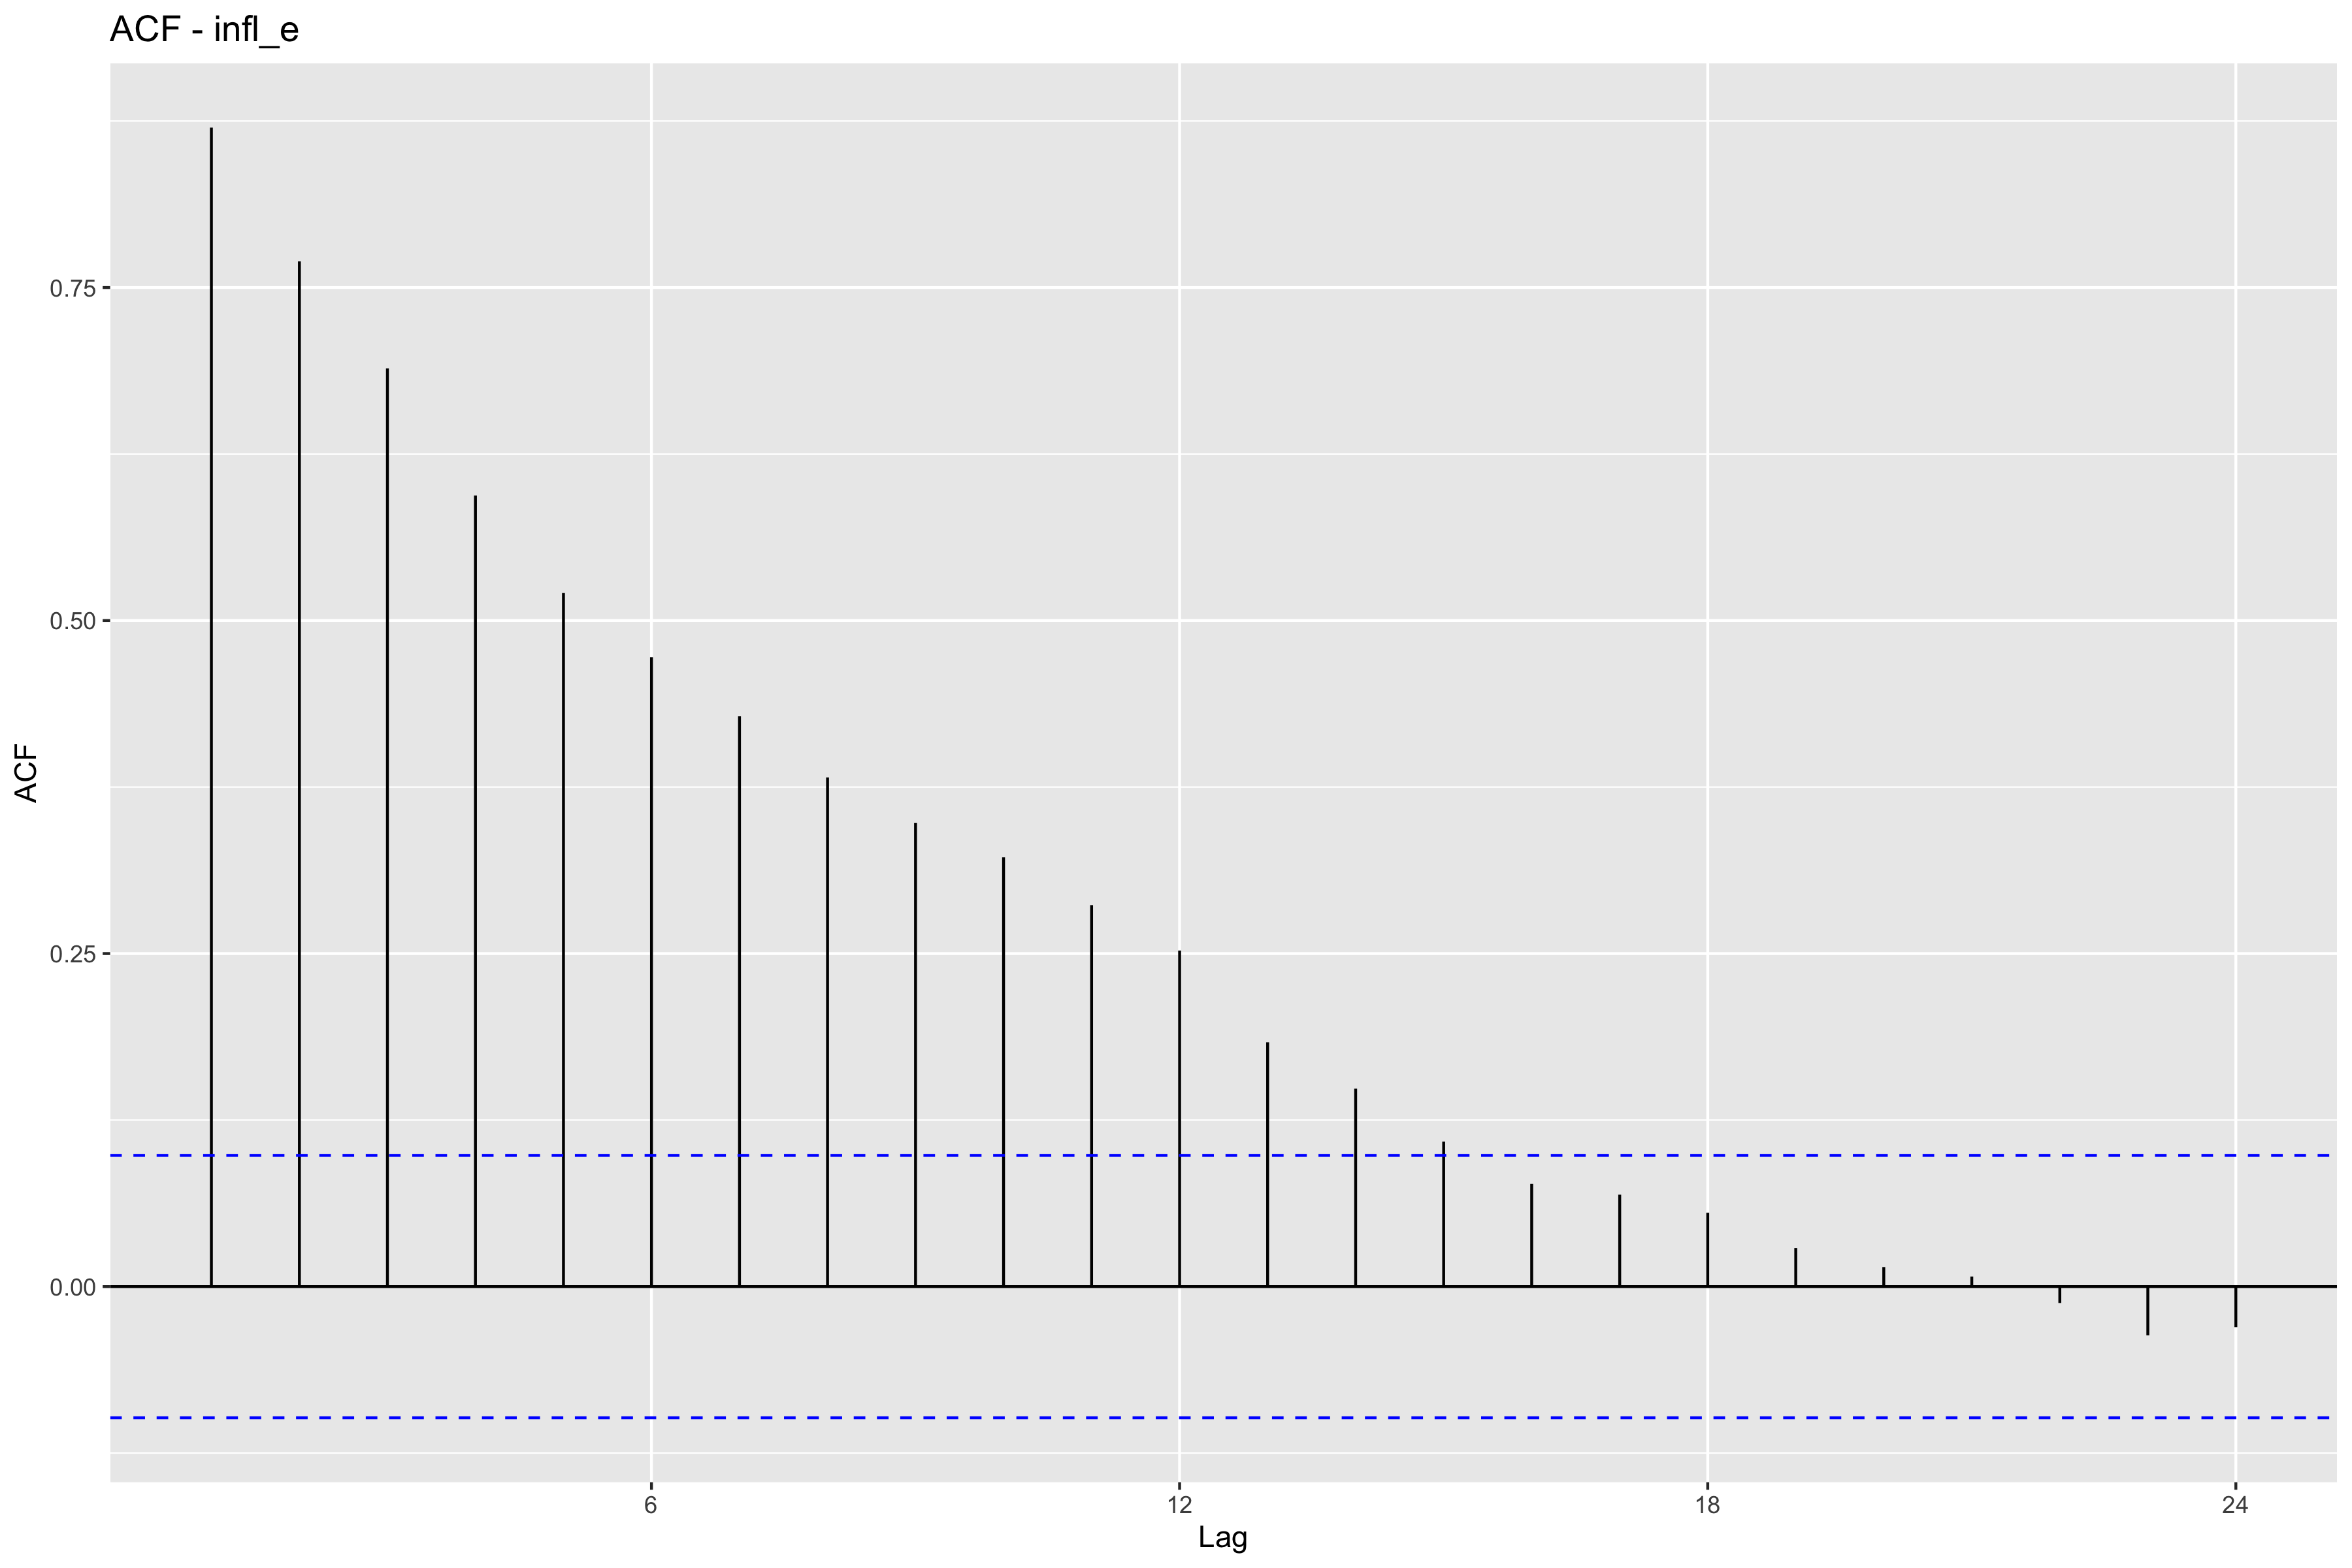
\includegraphics[width=\textwidth]{IMAGES/acf_infl.png}
        \caption*{Inflation expectation}
    \end{subfigure}
    \hfill
    \begin{subfigure}[b]{0.45\textwidth}
        \centering
        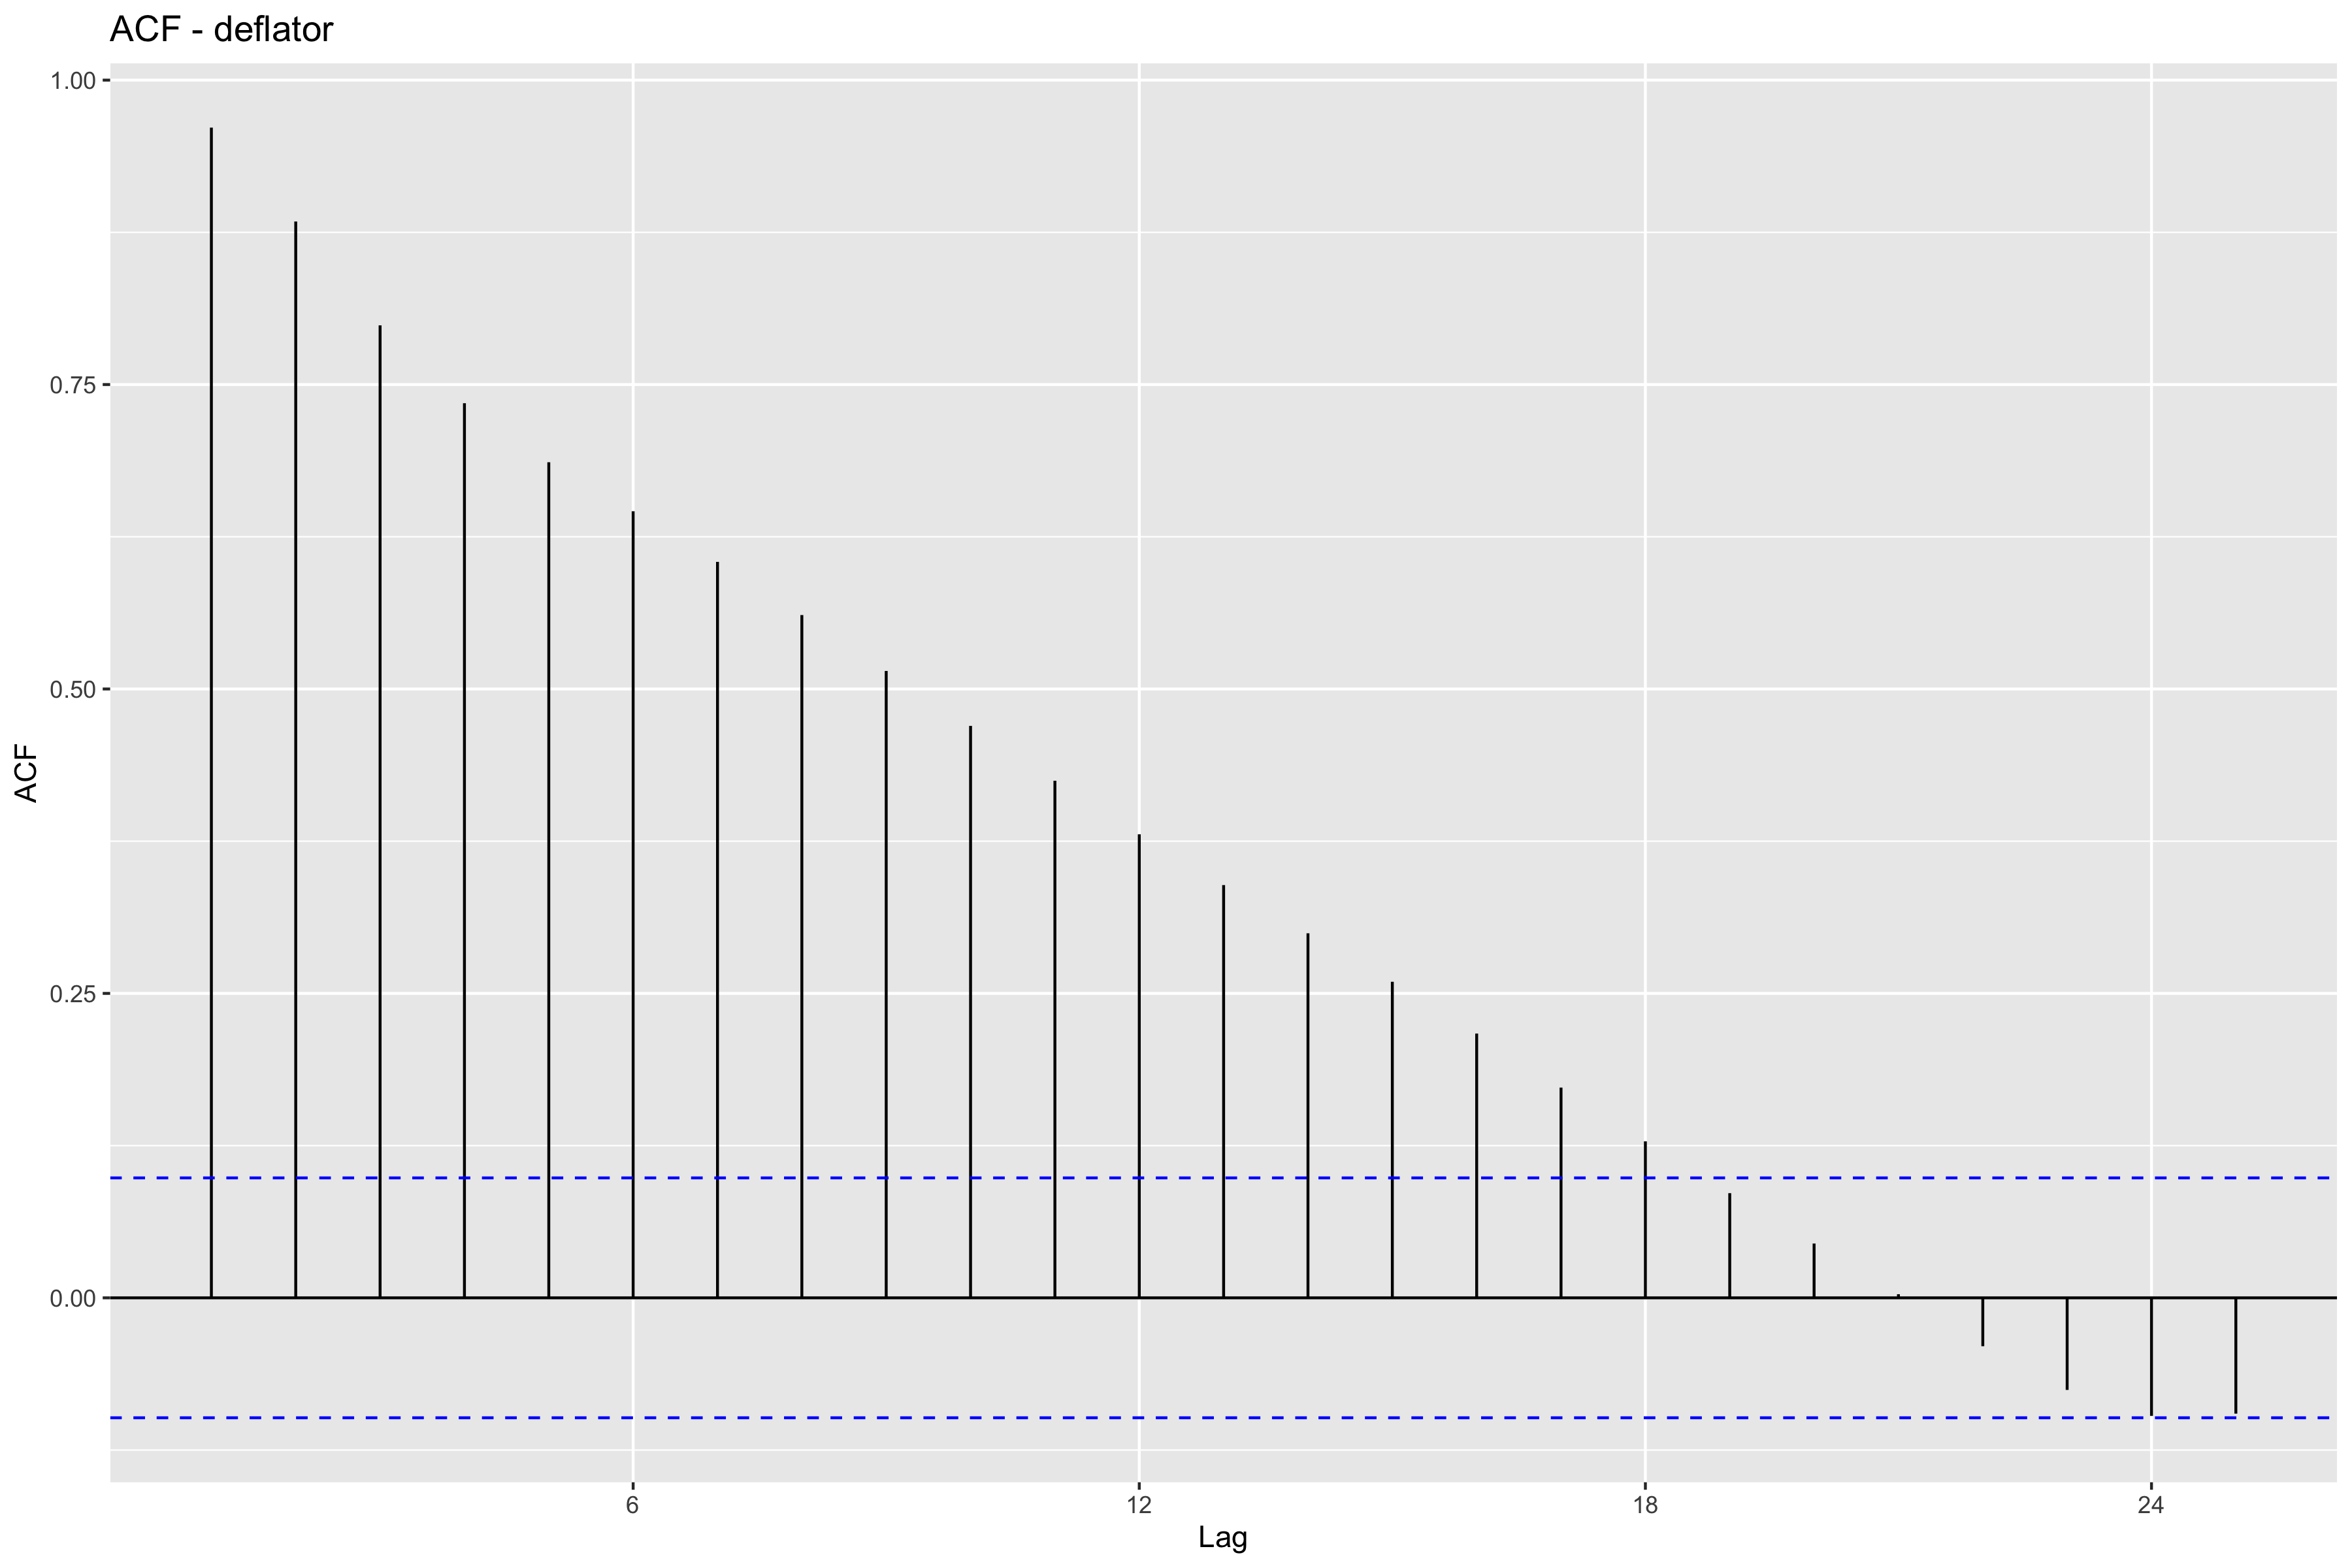
\includegraphics[width=\textwidth]{IMAGES/acf_defl.png}
        \caption*{GDP deflator}
    \end{subfigure}
    \hfill 
    \centering
    \begin{subfigure}[b]{0.45\textwidth}
        \centering
        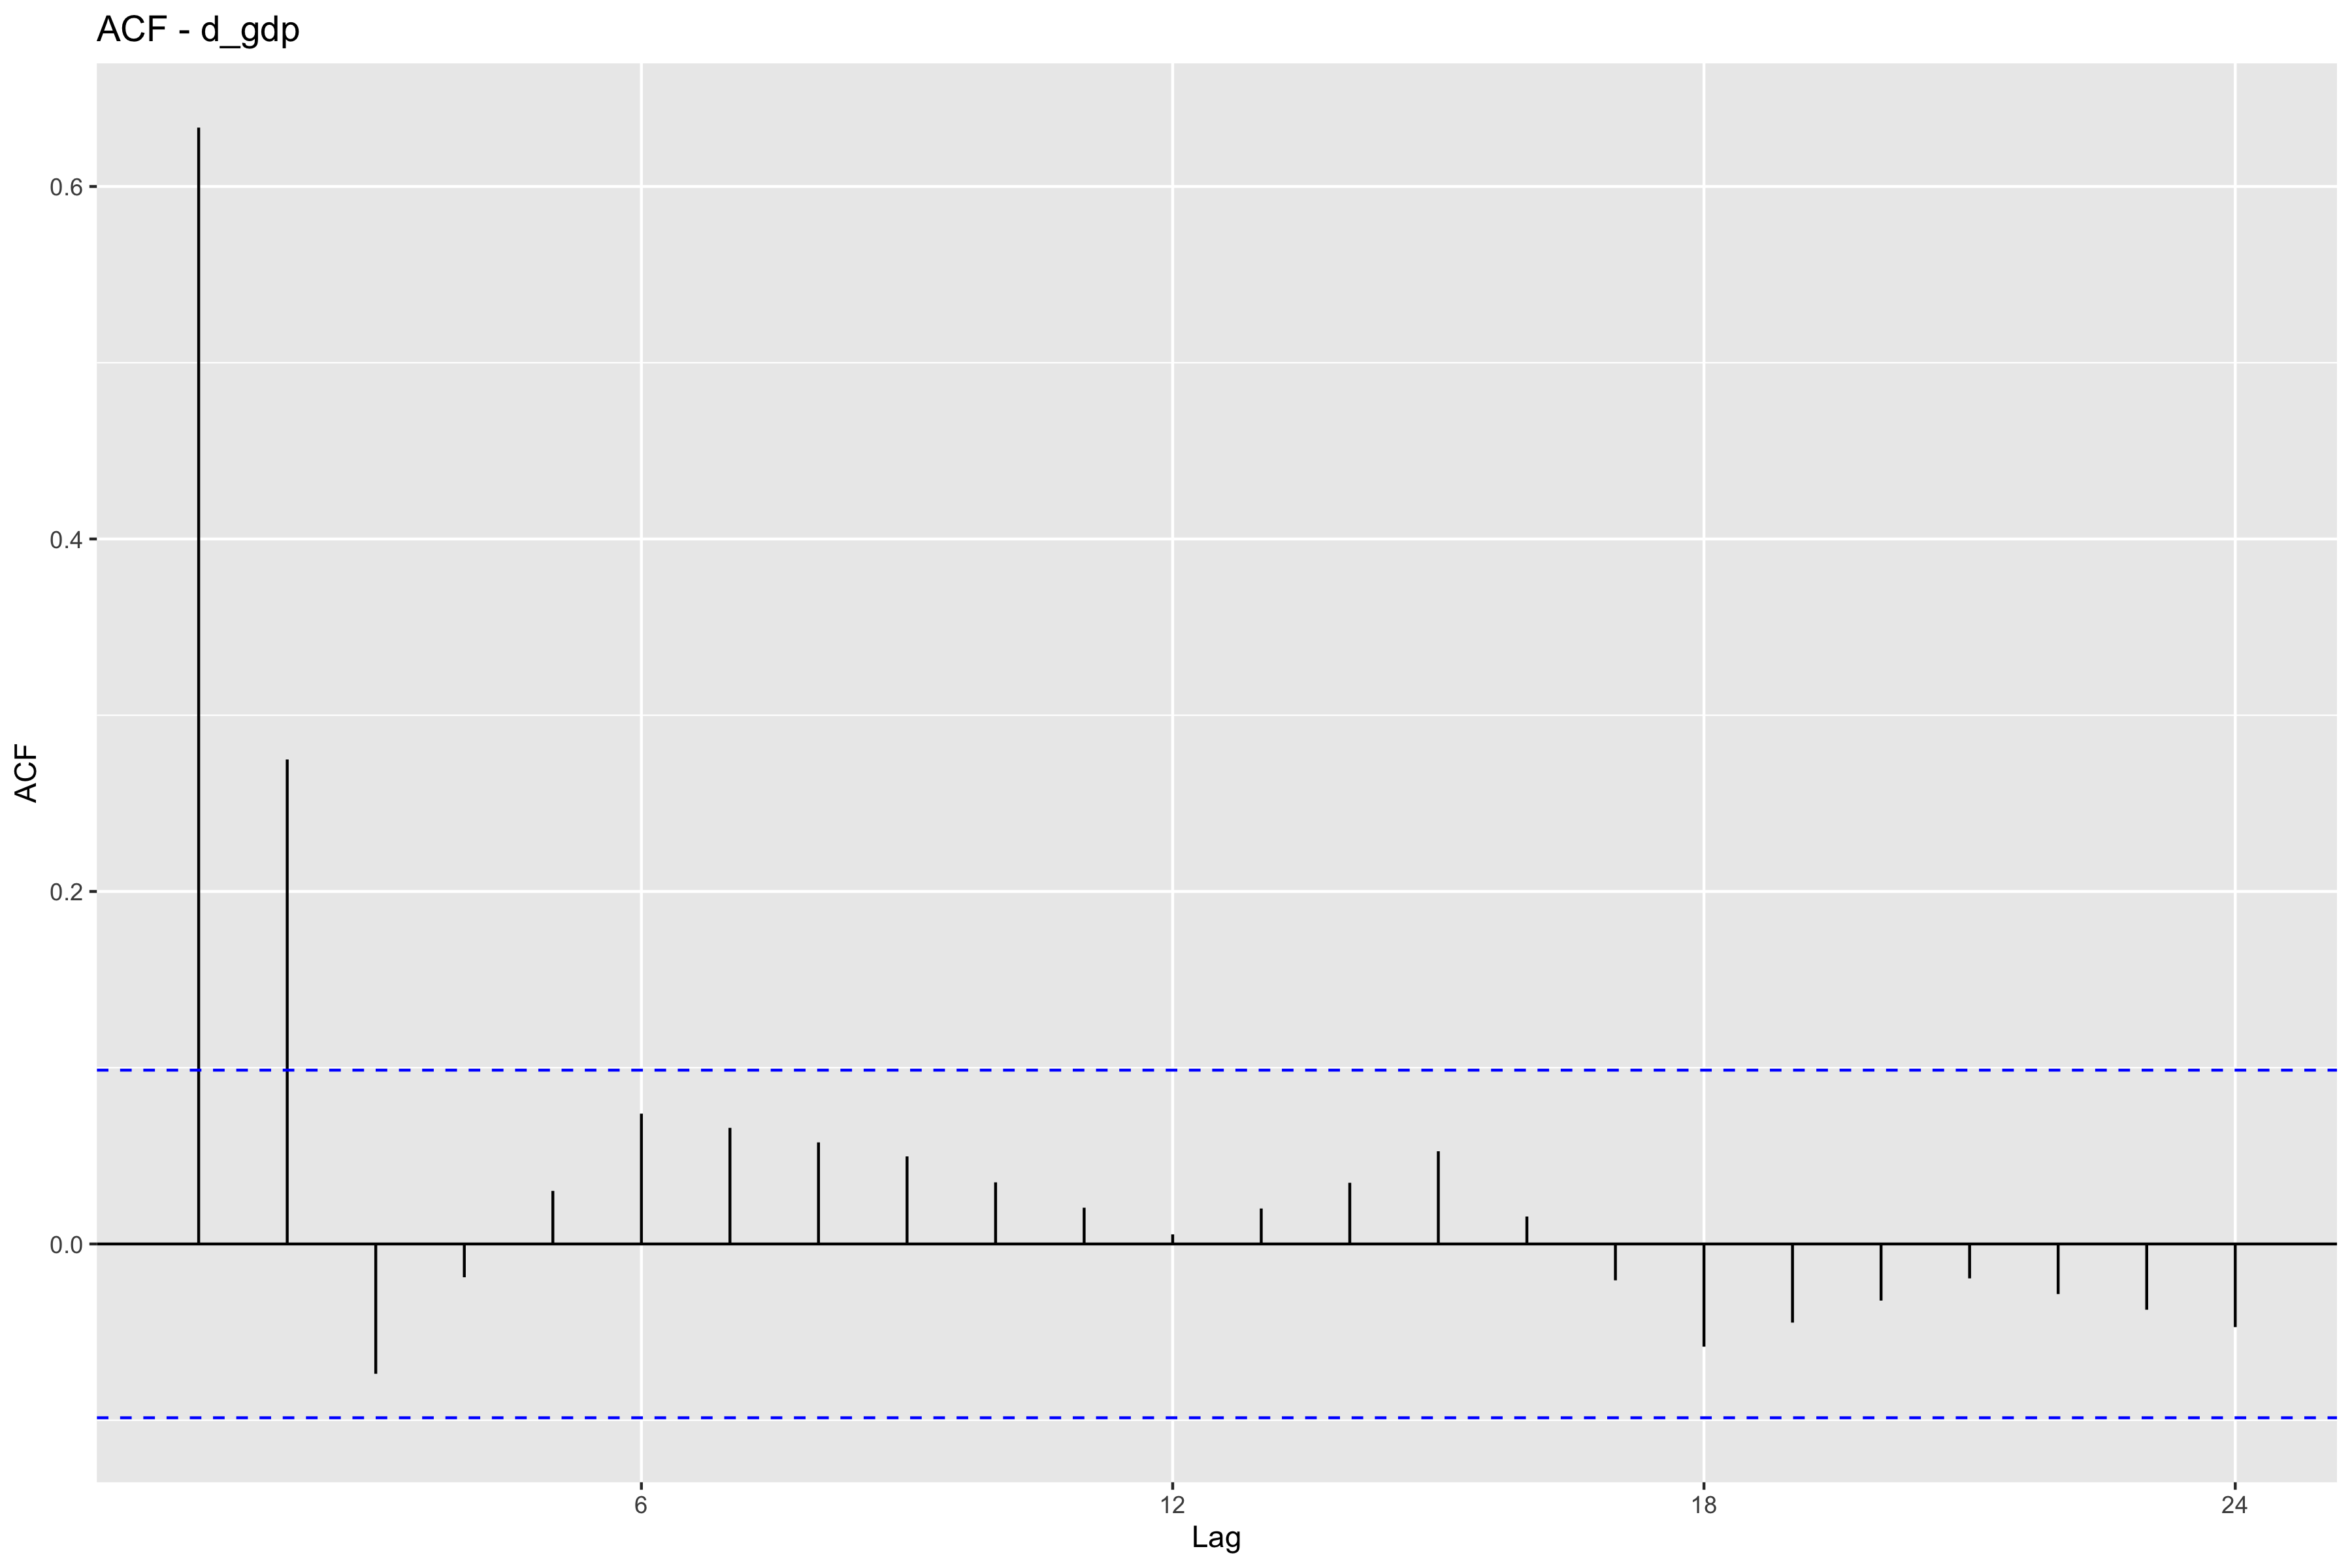
\includegraphics[width=\textwidth]{IMAGES/acf_gdp.png}
        \caption*{GDP growth rate}
    \end{subfigure}
    \hfill
    \begin{subfigure}[b]{0.45\textwidth}
        \centering
        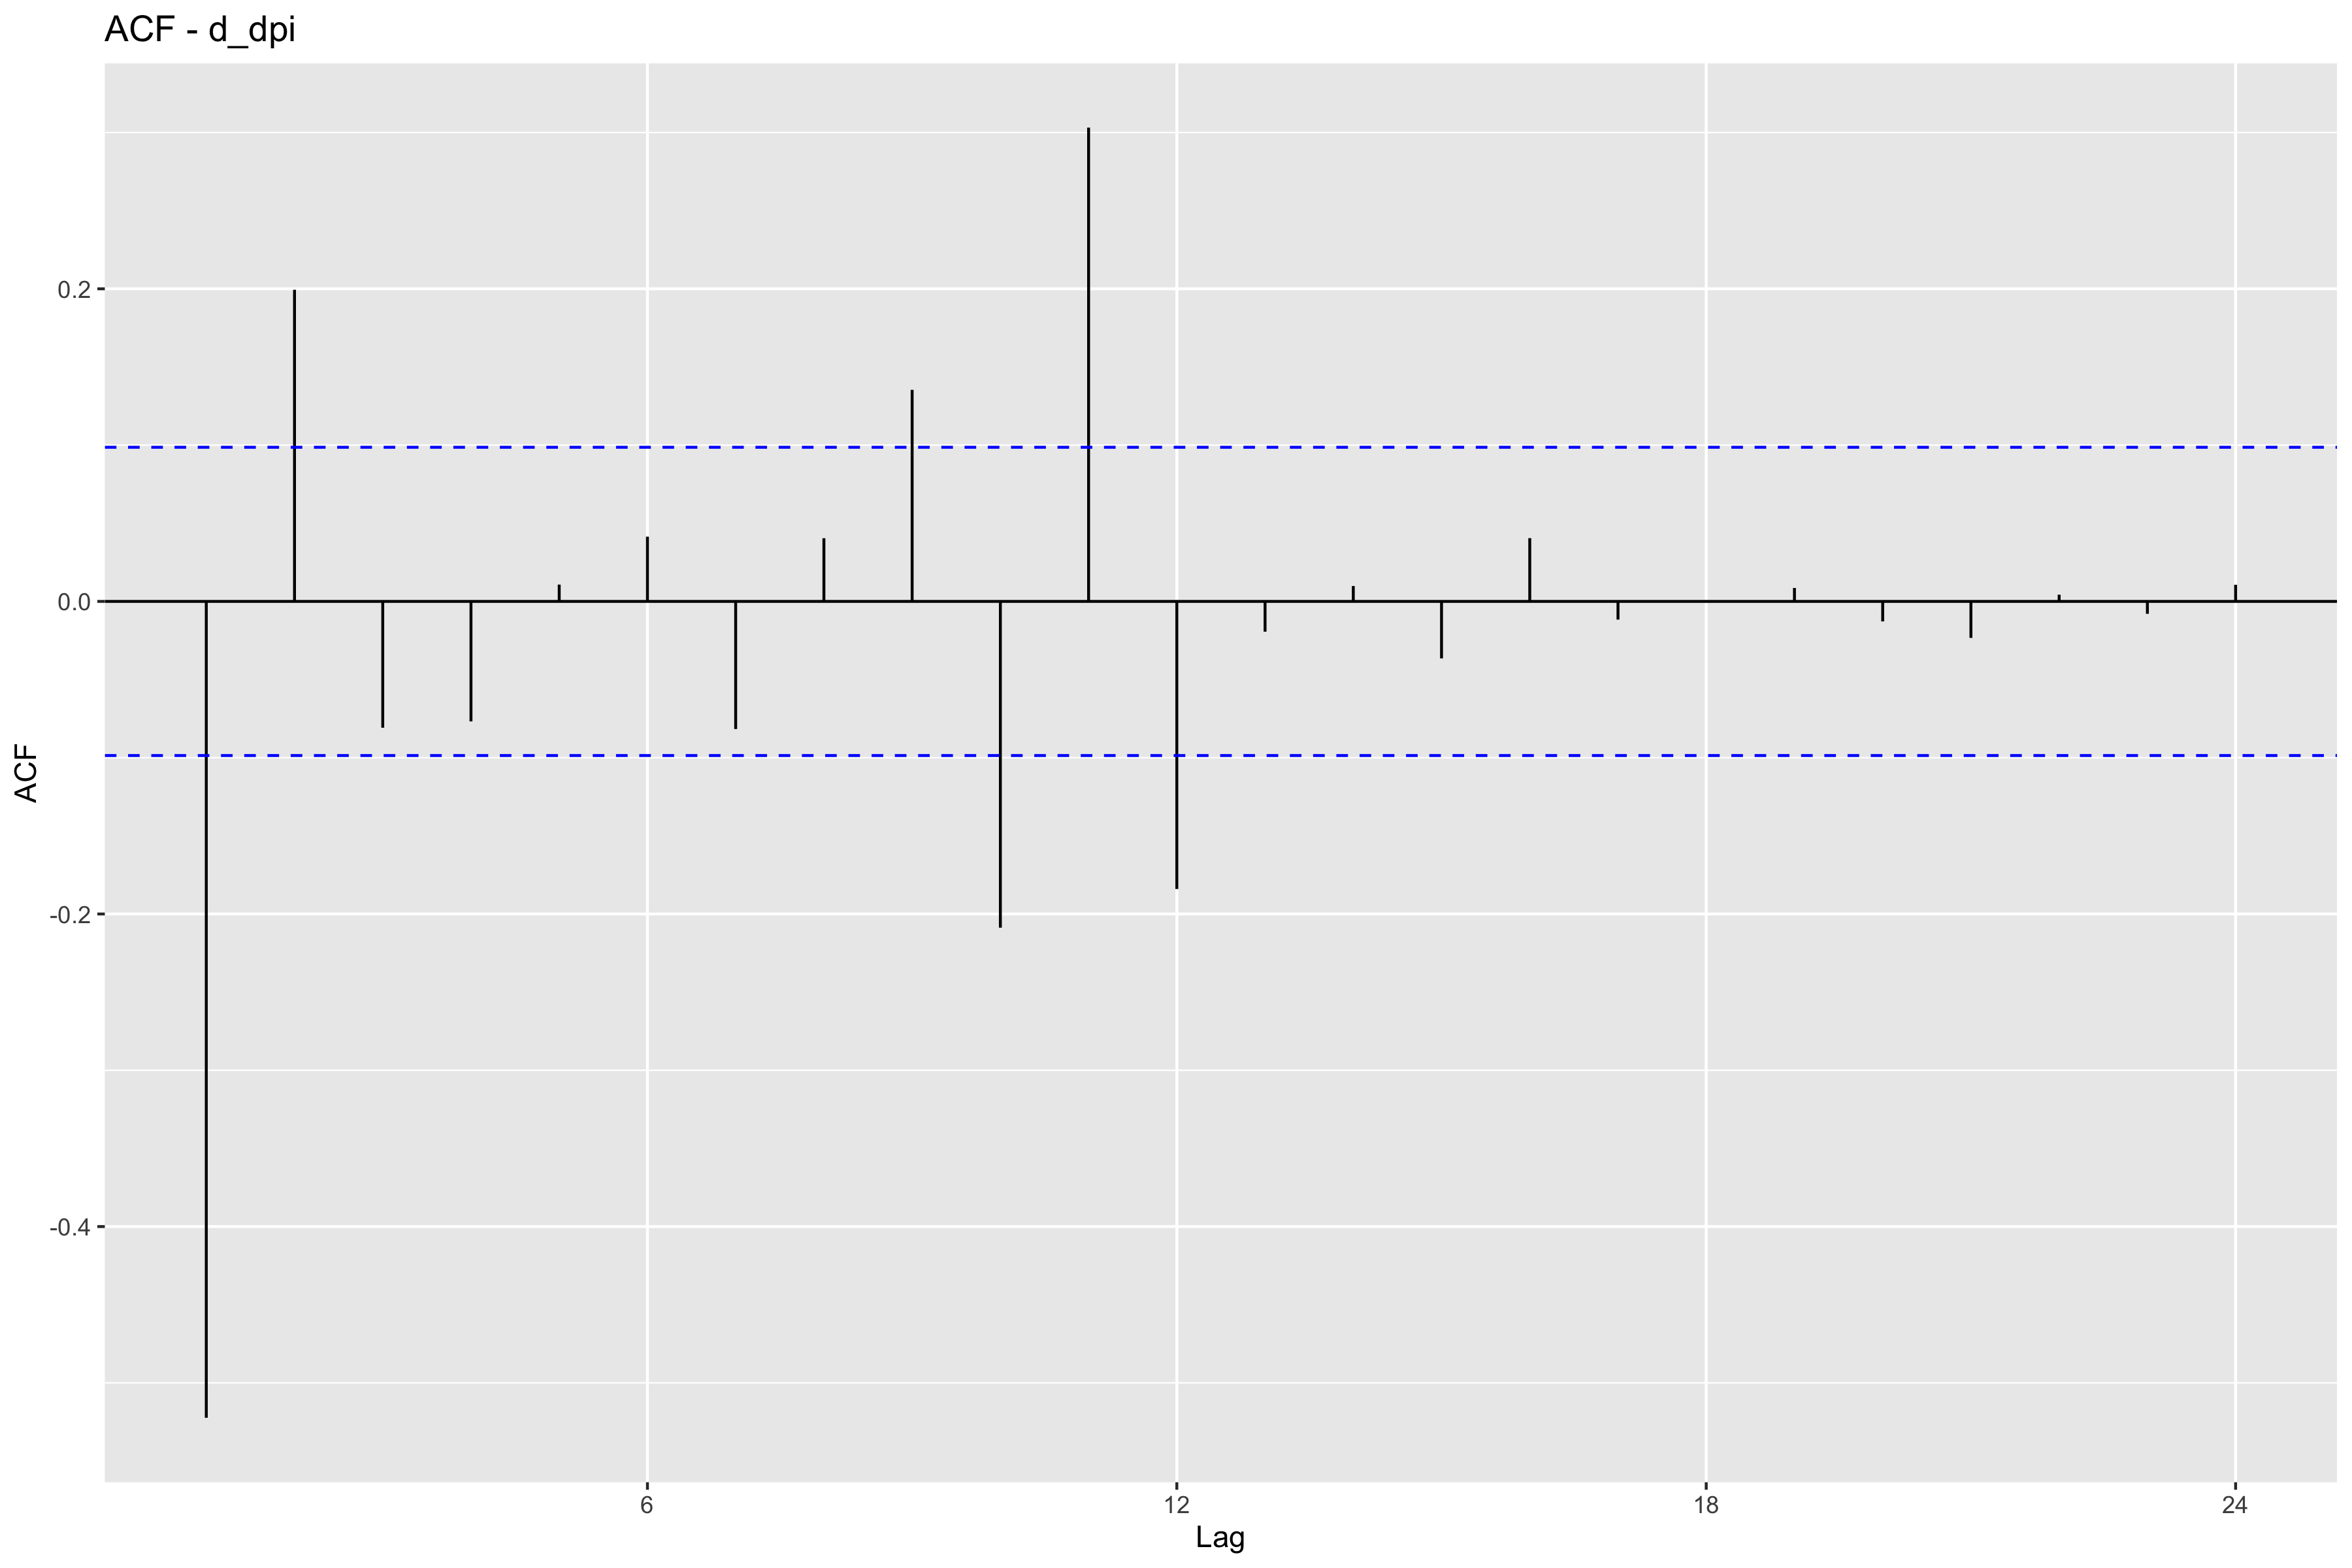
\includegraphics[width=\textwidth]{IMAGES/acf_dpi.png}
        \caption*{Real disponsable income growth rate }
    \end{subfigure}
    \hfill 
    \centering
    \begin{subfigure}[b]{0.45\textwidth}
        \centering
        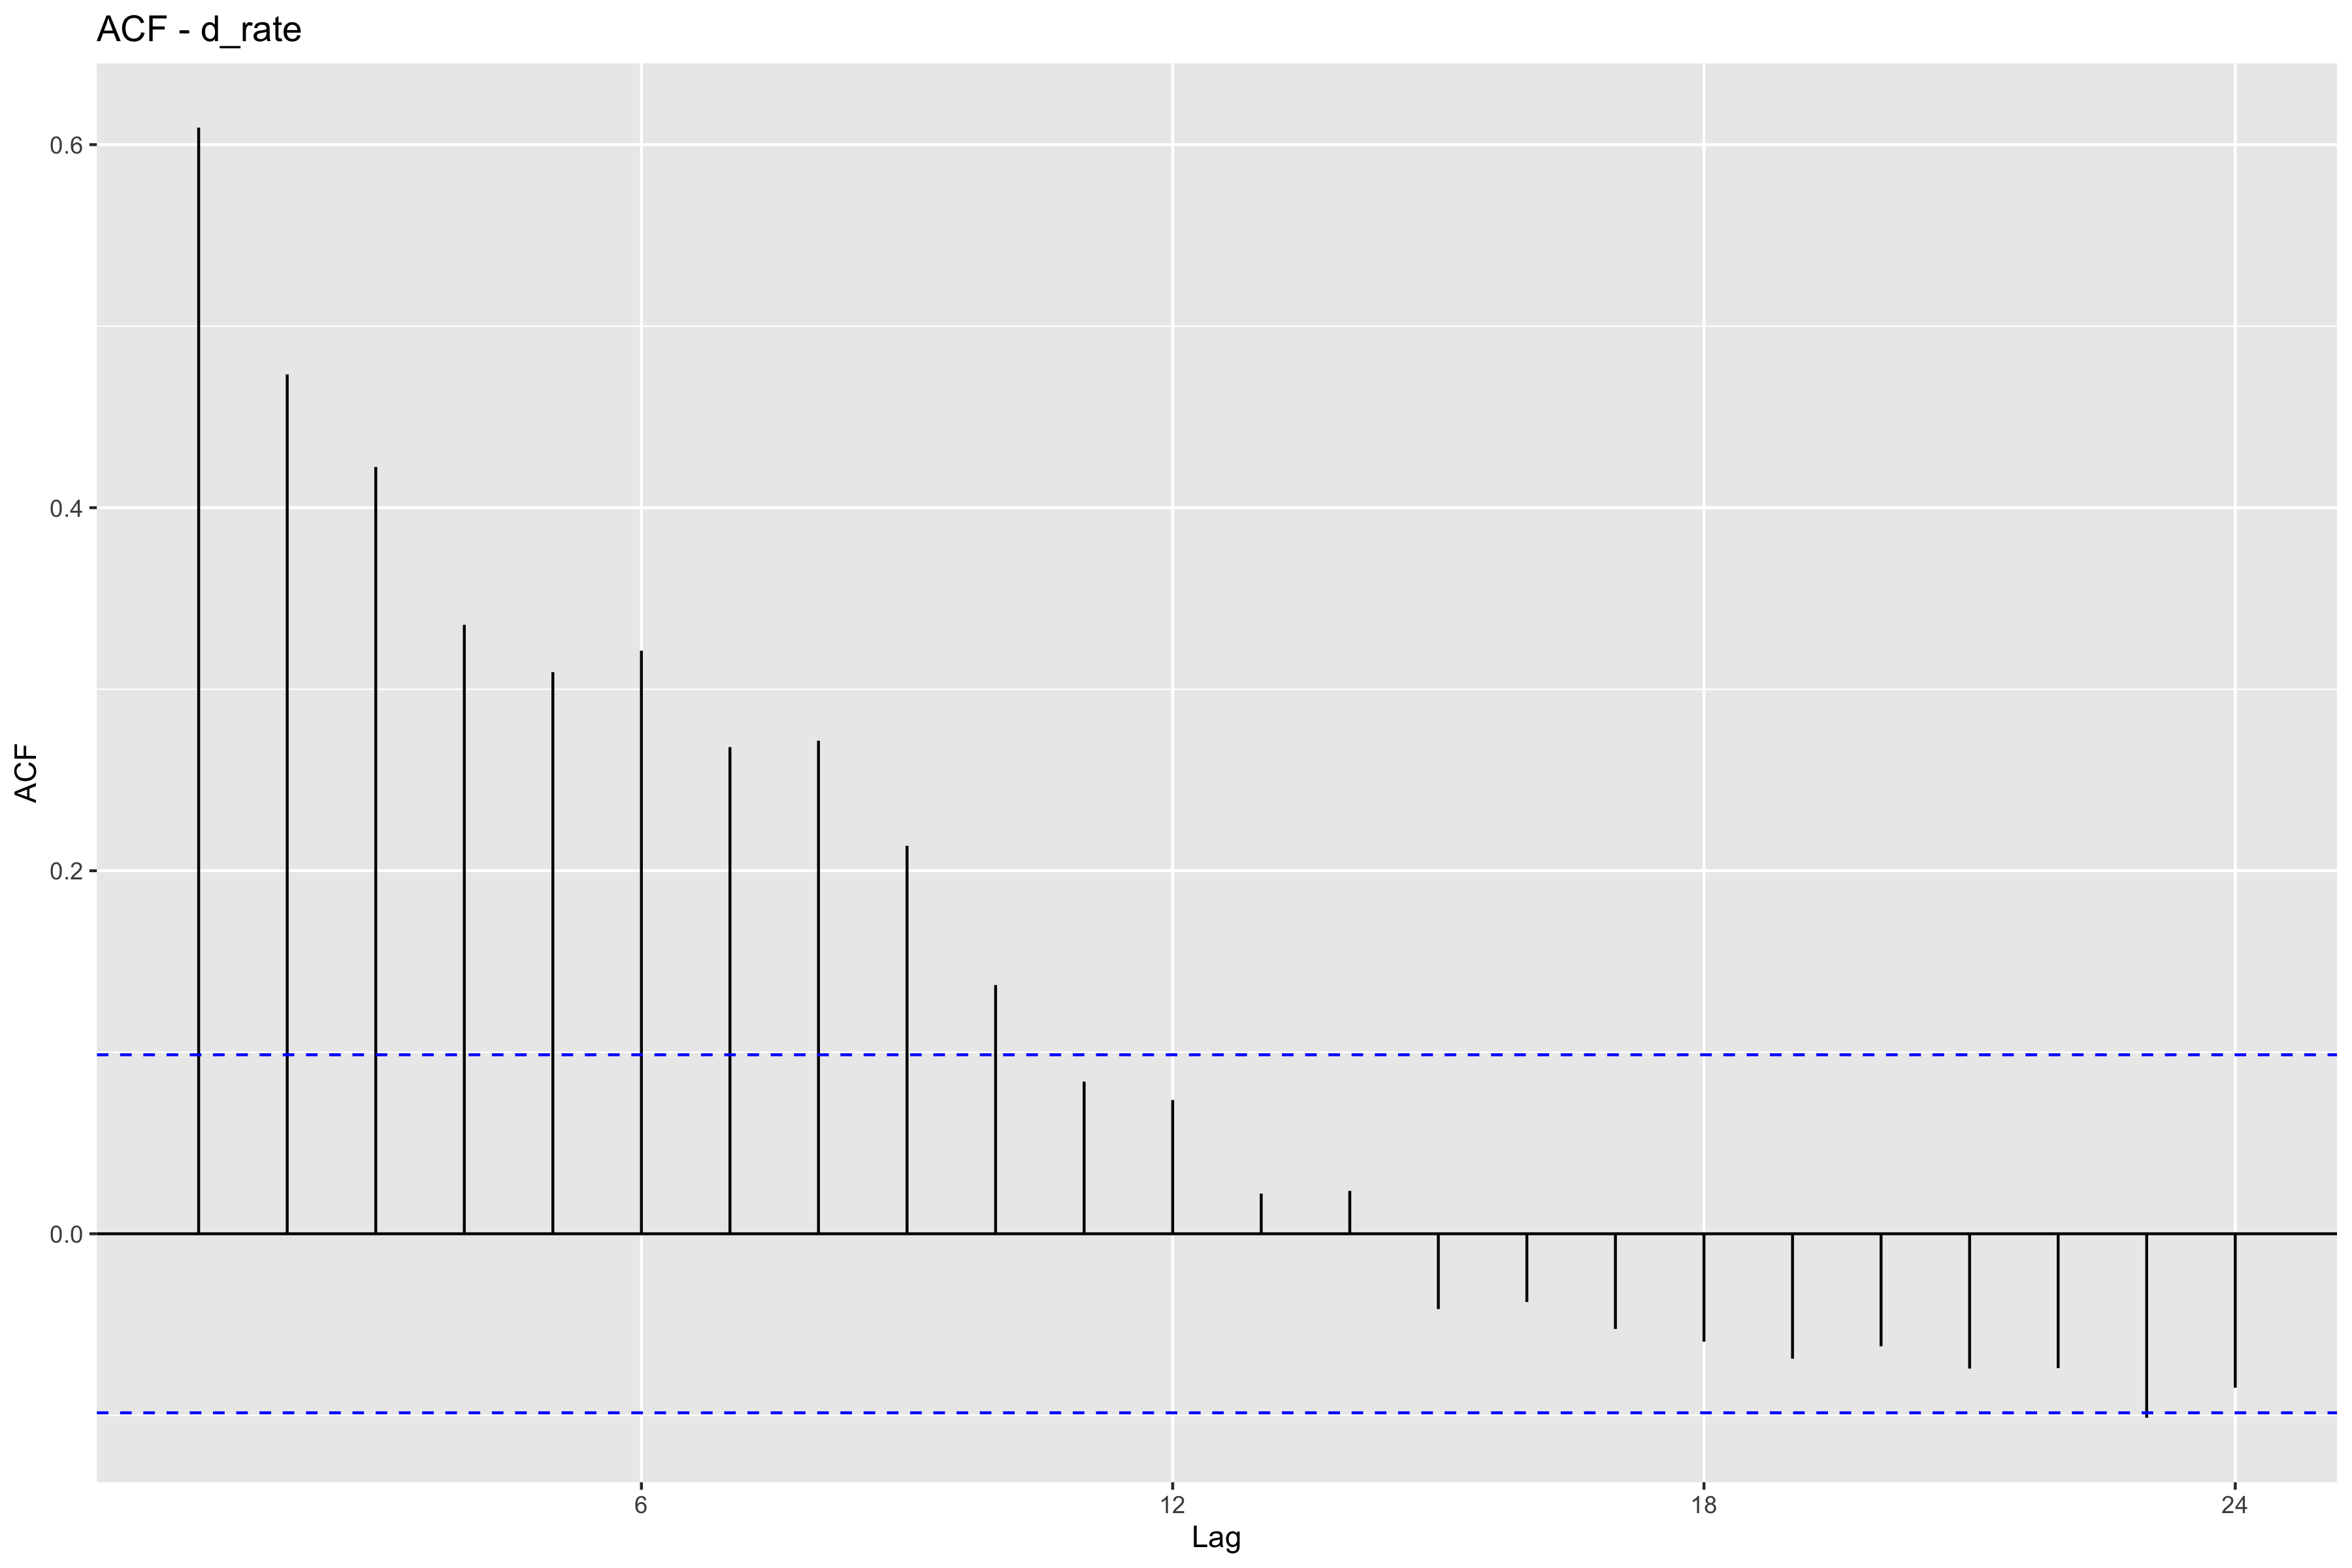
\includegraphics[width=\textwidth]{IMAGES/acf_rate.png}
        \caption*{Fed fund rate}
    \end{subfigure}
    \hfill
    \begin{subfigure}[b]{0.45\textwidth}
        \centering
        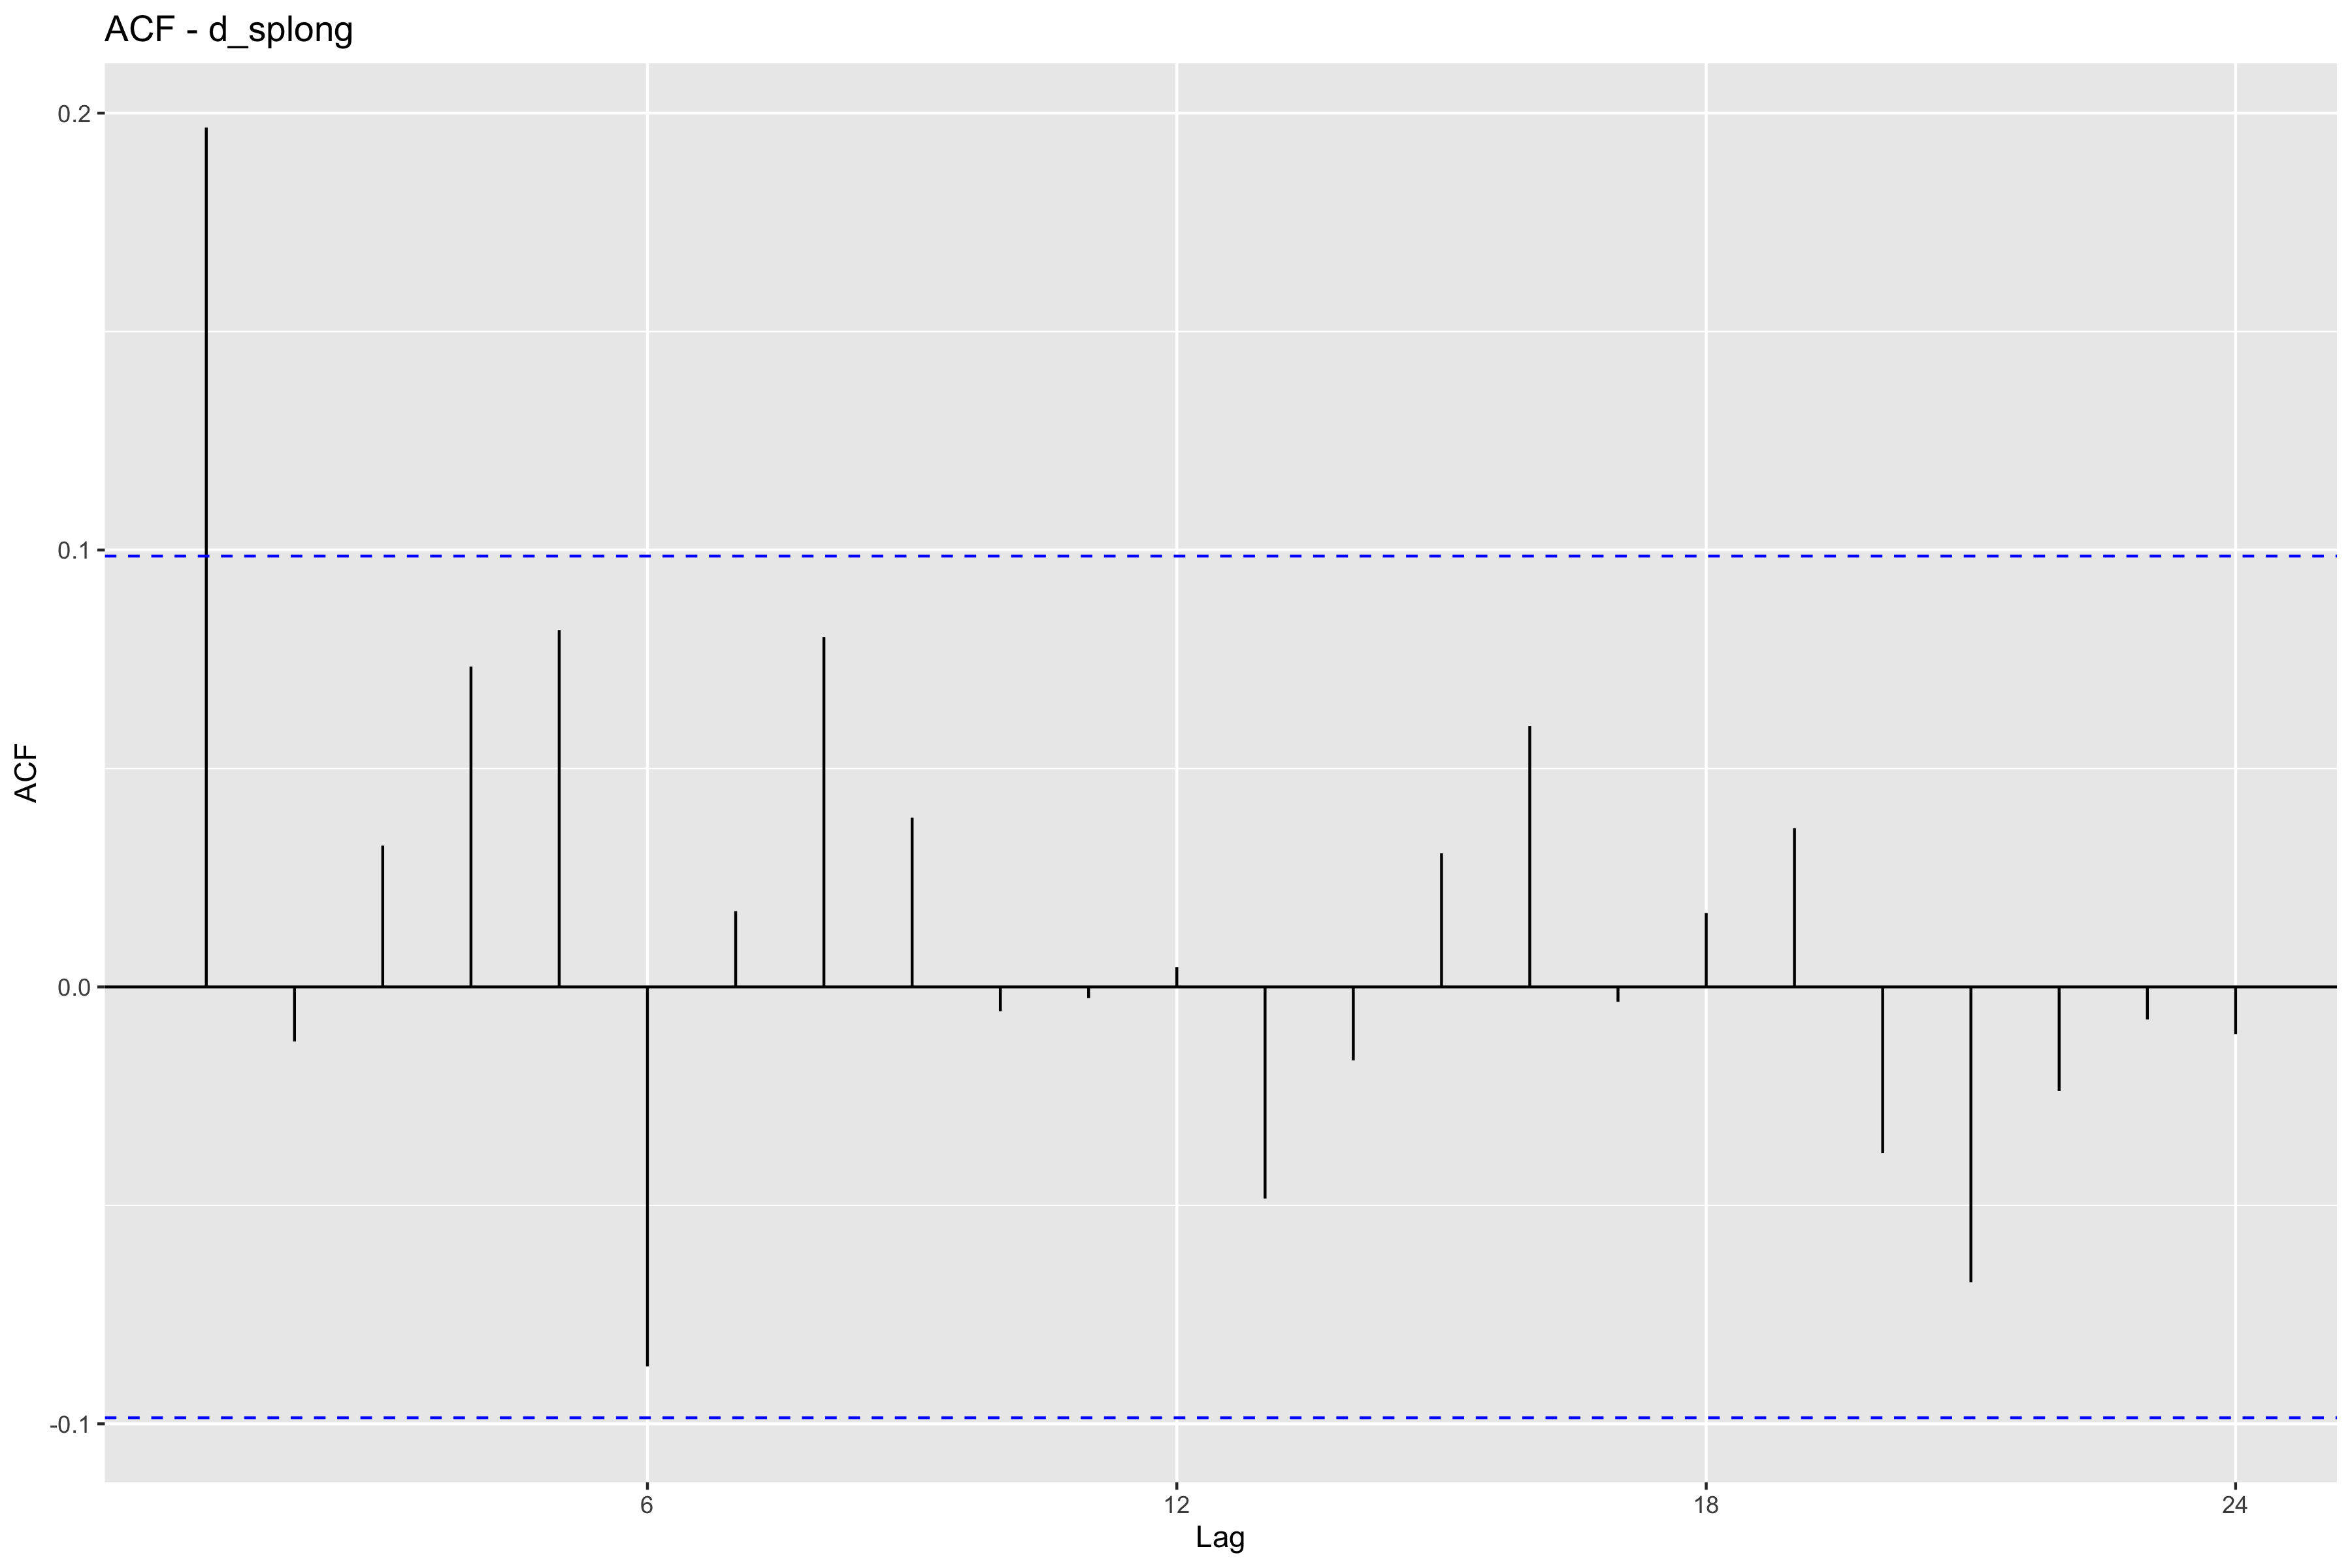
\includegraphics[width=\textwidth]{IMAGES/acf_sp.png}
        \caption*{Returns of S\&P500}
    \end{subfigure}
    \hfill 
    \caption{ACFs}
    \label{fig:acf_all}
    \begin{minipage}{0.9\textwidth}
        %\footnotesize
        \small{\emph{Notes}: All the series plotted are stationary: inflation expectation and GDP deflator series are in levels while the rest are first differences.}
    \end{minipage}
\end{figure}

We then find the best parameters for each model by minimizing the BIC (an informational criteria) for each combination of $p \leq \bar{p}$ and $ \leq \bar{q}$. 
This will allow us to find a combination of both types of models (AR and MA) such that we capture well the past with less parameters to estimate.
To do so, we use R's \texttt{critMatrix} function with the option \texttt{criteria = 'bic'}. 
Importantly, this operation is slow in particular when $\bar{p}, \bar{q}$ are both large. In the case of the inflation expectation and the first difference of the Fed fund rate, their values were so large that R does not give any answer and reports an error. 
To solve this, we decided to take smaller values of $\bar{p}$. Indeed, by looking at the PACF graphs (Figure \ref{fig:pacf_all}), we see that in both cases there is a single lag down the line that is significantly different from zero after several ones falling in the CI (lag 13 for \emph{infl-e} and lag 15 for \emph{d-rate}). 
We took the previous significant lag as $\bar{p}$ to be able to get the information criteria with the rationale that those "extreme" significant lags can be due to just luck, and that the combination of AR and MA models should allow to reduce the number of parameters. 

We present the outputs of these comparitions tables per series in Appendix \ref{sec:BIC_tables} because they are a lot and they were making hard to read this section. 
Remark that the palcement of the $p$s and $q$s can vary from one tabel to the next due to formatting issues. 
We find that the orders $p$ and $q$ that minimize the nformation criteria are: 
    \begin{itemize}
        \item[-] Inflation expectation: $ARMA(1,0)$ (BIC = $236.04$)
        \item[-] GDP Deflator: $ARMA(2,1)$ (BIC = 164.23)  
        \item[-] GDP growth rate (\emph{d-gdp}): $ARMA(0,2)$ (BIC = -3556.28)
        \item[-] Real disposable income growth rate (\emph{d-dpi}): $ARMA(2,1)$ (BIC=-2161.22)
        \item[-] Fed Fund rate (\emph{d-rate}): $ARMA(1,1)$ (BIC = -413.58)
        \item[-] S\&P500 rate (\emph{d-splong}): $ARMA(0,1)$ (BIC = -1509.36)
    \end{itemize}

With this information we can finally estimate these ARMA models using R's \texttt{arima} function. 
Since all the series are stationary, we just set $d=0$ and the ARIMA models become ARMA. 
We get the following resuts: 

% Table created by stargazer v.5.2.3 by Marek Hlavac, Social Policy Institute. E-mail: marek.hlavac at gmail.com
% Date and time: Wed, Dec 13, 2023 - 05:06:04
\begin{table}[!htbp] \centering 
  \caption{ARMA model for the cyclical components} 
  \label{tab:all_arma} 
\begin{tabular}{@{\extracolsep{5pt}}lcccccc} 
\\[-1.8ex]\hline 
\hline \\[-1.8ex] 
 & \multicolumn{6}{c}{\textit{Dependent variable:}} \\ 
\cline{2-7} 
\\[-1.8ex] &  infl\_e & deflator  & d\_gdp  & d\_dpi  &d\_rate  & d\_splong \\ 
\\[-1.8ex] & (1) & (2) & (3) & (4) & (5) & (6)\\ 
\hline \\[-1.8ex] 
 ar1 & 0.881$^{***}$ & $-$0.110$^{***}$ &  & 0.160 & 0.855$^{***}$ &  \\ 
  & (0.024) & (0.024) &  & (0.107) & (0.045) &  \\ 
  & & & & & & \\ 
 ar2 &  & 0.886$^{***}$ &  & 0.268$^{***}$ &  &  \\ 
  &  & (0.024) &  & (0.080) &  &  \\ 
  & & & & & & \\ 
 ma1 &  & 0.986$^{***}$ & 0.939$^{***}$ & $-$0.770$^{***}$ & $-$0.418$^{***}$ & 0.214$^{***}$ \\ 
  &  & (0.010) & (0.024) & (0.089) & (0.083) & (0.051) \\ 
  & & & & & & \\ 
 ma2 &  &  & 0.881$^{***}$ &  &  &  \\ 
  &  &  & (0.026) &  &  &  \\ 
  & & & & & & \\ 
 intercept & 0.178 & 0.182 & 0.0004 & $-$0.005$^{***}$ & 0.027 & $-$0.005$^{**}$ \\ 
  & (0.134) & (0.140) & (0.0004) & (0.0003) & (0.028) & (0.002) \\ 
  & & & & & & \\ 
\hline \\[-1.8ex] 
Observations & 396 & 396 & 395 & 395 & 395 & 395 \\ 
Log Likelihood & $-$115.027 & $-$110.948 & 1,784.121 & 1,089.580 & 212.271 & 757.671 \\ 
$\sigma^{2}$ & 0.104 & 0.102 & 0.00001 & 0.0002 & 0.020 & 0.001 \\ 
Akaike Inf. Crit. & 236.054 & 231.897 & $-$3,560.241 & $-$2,169.159 & $-$416.542 & $-$1,509.341 \\ 
\hline 
\hline \\[-1.8ex] 
\textit{Note:}  & \multicolumn{6}{r}{$^{*}$p$<$0.1; $^{**}$p$<$0.05; $^{***}$p$<$0.01} \\ 
\end{tabular} 
\end{table} 


Finally, we check that the residuals of the models aren't serially correlated using the Ljung–Box test that is available with R's \texttt{Box.test} function.
This test poses as a null hypothesis H0 that the data tested is independently distributed i.e. in this case, since we test the residuals, that there is no serial correlation between them.
The test results are found in Table \ref{tab:ljungbox}

% latex table generated in R 4.3.1 by xtable 1.8-4 package
% Wed Dec 13 05:43:36 2023
\begin{table}[ht]
  \caption{Ljung-Box test: p-values}
  \label{tab:ljungbox}
\centering
\begin{tabular}{rlr}
  \hline
 & Model & p-value \\ 
  \hline
 & infl\_e & 0.20 \\ 
   & deflator & 0.04 \\ 
   & d\_gdp & 0.94 \\ 
   & d\_dpi & 0.01 \\ 
   & d\_rate & 0.08 \\ 
   & d\_splong & 0.25 \\ 
   \hline
\end{tabular}
\end{table}


We cannot reject the null hypothesis in most of the models (p-values $< 0.05$) leading us to support the idea that for the inflation expectation, GDP growth, Fed fund rate and the return rate of the S\&P500, the ARMA models that we proposed before correctly captures the auto-correlation structure of their cyclical components.
However, we do reject H0 for the GDP deflator and the growth rate of disposable personal income suggesting that our models are not adequate. 
We couldn't find where the error might lie. 











\newpage
\newpage
\section{VARs}

\textcolor{gray}{In this section we introduce several Vector Autoregressive models (VAR) corresponding to applications 2,3 and 4.}

When it comes to economic fluctuations and financial market volatility, understanding the complex dynamics between financial indices and macroeconomic indicators is becoming increasingly crucial. This report aims to do an empirical analysis in the field of financial econometrics.Precisely, it employs a Vector Autoregression (VAR) model to examine the interactions among three key economic variables: the long-term S\&P 500 index (splong), a key index of the US Stock Market that represents the 500 largest companies by market cap, the Gross Domestic Product (gdp), and the Federal Reserve interest rate (rate), both of course of the United States. These three were chosen for their pronounced non-stationary characteristics and significant impact on economic analysis, and in the world itself, given that they all come from the largest economy in the world.

%Utilizing the Augmented Dickey-Fuller (ADF) test, we analyzed these series for unit roots to determine their integration order. This step is essential in developing an accurate and reliable VAR model. The modeling of these series in levels or first differences depends on the ADF test outcomes, ensuring the model accurately reflects the data's time-dependent structure.

This part of the empirical application, aims to uncover the complex relationships among these financial and macroeconomic variables. The main goal, is to have a better understanding of their collective behavior.


\subsection{Stationarity of the series}

We used series some of the series that  we introduced and analyzed in the previous section.
We let teh reader go back to see the full procedure regarding the test of UR fir the series in question. 
We shall recall that all three series of interest in this section i.e. \texttt{splong, rate \text{and} gdp} are I(1) series meaning that we would not be able to implement a Canonical VAR in levels. 
We shall test for cointegration among the series to know if we can implement an error correcting version of the VAR models (VECM) that manages to handle and correct the errors induced by the presence of UR in the series with linear combinations of their stochastic trends. 
If we do not find a cointegration relationship between the series, we need to move to a VAR using the series of first differences that are stationary. 

\subsection{Cointegration test}

\begin{figure}[h!]
    \centering
    \includegraphics*[width=0.75\textwidth]{IMAGES/coint_test.png}
    \caption{Cointegration: Johansen test}
\end{figure}





\begin{table}[htbp]
    \centering
    \caption{Granger Causality Test Results}
    \begin{tabular}{|l|c|c|}
    \toprule
    \textbf{Causality Test} & \textbf{F-Test} & \textbf{p-value} \\
    \midrule
    gdp $\rightarrow$ splong rate & $5.8032$ & $4.724 \times 10^{-11}$ \\
    splong $\rightarrow$ gdp rate & $2.844$ & $0.0003251$ \\
    rate $\rightarrow$ splong gdp & $3.7709$ & $2.993 \times 10^{-06}$ \\
    \bottomrule
    \end{tabular}
    \label{tab:granger_results}
\end{table}












\newpage
\section{Introduce non-linearities}\label{sec:nonlinearities}
    \subsection{Markov-switching model}\label{sec:markov}

    
    \subsection{STR model}\label{sec:str}



%\section{Difference-in-Difference}
%https://www.tidy-finance.org/r/difference-in-differences.html
    



\newpage
\newpage
\begin{appendices}

    \section{Section 1 - Additional tables} \label{sec:BIC_tables}
    
% Table created by stargazer v.5.2.3 by Marek Hlavac, Social Policy Institute. E-mail: marek.hlavac at gmail.com
% Date and time: Tue, Dec 12, 2023 - 16:56:05
\begin{table}[!htbp] \centering 
  \caption{Information criteria on the parameters of ARMA for infl_e} 
  \label{tab:bic_infl} 
\begin{tabular}{@{\extracolsep{5pt}} cccccc} 
\\[-1.8ex]\hline 
\hline \\[-1.8ex] 
 & p=0 & p=1 & p=2 & p=3 & p=4 \\ 
\hline \\[-1.8ex] 
q=0 & $808.438$ & $236.035$ & $239.455$ & $244.671$ & $246.751$ \\ 
q=1 & $517.737$ & $239.263$ & $239.841$ & $244.875$ & $252.676$ \\ 
q=2 & $413.415$ & $245.105$ & $244.731$ & $249.439$ & $254.721$ \\ 
q=3 & $348.231$ & $247.220$ & $249.095$ & $254.601$ & $254.129$ \\ 
q=4 & $298.207$ & $252.154$ & $246.078$ & $259.082$ & $265.384$ \\ 
q=5 & $292.940$ & $254.133$ & $246.824$ & $251.856$ & $258.027$ \\ 
q=6 & $289.687$ & $259.915$ & $252.000$ & $257.838$ & $262.286$ \\ 
q=7 & $278.591$ & $265.863$ & $257.687$ & $263.809$ & $264.647$ \\ 
q=8 & $275.739$ & $270.725$ & $262.675$ & $266.930$ & $270.434$ \\ 
q=9 & $281.720$ & $276.114$ & $264.761$ & $270.662$ & $274.023$ \\ 
q=10 & $284.970$ & $277.918$ & $270.633$ & $271.776$ & $278.872$ \\ 
q=11 & $289.458$ & $283.842$ & $275.724$ & $276.490$ & $283.533$ \\ 
q=12 & $284.137$ & $277.990$ & $279.720$ & $282.047$ & $289.110$ \\ 
q=13 & $286.646$ & $283.125$ & $279.067$ & $285.024$ & $290.893$ \\ 
q=14 & $288.837$ & $288.879$ & $285.013$ & $290.070$ & $288.811$ \\ 
q=15 & $292.928$ & $294.809$ & $290.843$ & $306.880$ & $298.582$ \\ 
\hline \\[-1.8ex] 
\end{tabular} 
\end{table} 


    
% Table created by stargazer v.5.2.3 by Marek Hlavac, Social Policy Institute. E-mail: marek.hlavac at gmail.com
% Date and time: Wed, Dec 13, 2023 - 04:34:38
\begin{table}[!htbp] \centering 
  \caption{Information criteria on the parameters of ARMA for GDP deflator} 
  \label{tab:bic_deflator} 
\begin{tabular}{@{\extracolsep{5pt}} cccccc} 
\\[-1.8ex]\hline 
\hline \\[-1.8ex] 
 & p=0 & p=1 & p=2 & p=3 & p=4 \\ 
\hline \\[-1.8ex] 
q=0 & $808.438$ & $236.035$ & $239.455$ & $244.671$ & $246.751$ \\ 
q=1 & $517.737$ & $239.263$ & $239.841$ & $244.875$ & $252.676$ \\ 
q=2 & $413.415$ & $245.105$ & $244.731$ & $249.439$ & $254.721$ \\ 
q=3 & $348.231$ & $247.220$ & $249.095$ & $254.601$ & $254.129$ \\ 
q=4 & $298.207$ & $252.154$ & $246.078$ & $259.082$ & $265.384$ \\ 
q=5 & $292.940$ & $254.133$ & $246.824$ & $251.856$ & $258.027$ \\ 
q=6 & $289.687$ & $259.915$ & $252.000$ & $257.838$ & $262.286$ \\ 
q=7 & $278.591$ & $265.863$ & $257.687$ & $263.809$ & $264.647$ \\ 
q=8 & $275.739$ & $270.725$ & $262.675$ & $266.930$ & $270.434$ \\ 
q=9 & $281.720$ & $276.114$ & $264.761$ & $270.662$ & $274.023$ \\ 
q=10 & $284.970$ & $277.918$ & $270.633$ & $271.776$ & $278.872$ \\ 
q=11 & $289.458$ & $283.842$ & $275.724$ & $276.490$ & $283.533$ \\ 
q=12 & $284.137$ & $277.990$ & $279.720$ & $282.047$ & $289.110$ \\ 
q=13 & $286.646$ & $283.125$ & $279.067$ & $285.024$ & $290.893$ \\ 
q=14 & $288.837$ & $288.879$ & $285.013$ & $290.070$ & $288.811$ \\ 
q=15 & $292.928$ & $294.809$ & $290.843$ & $306.880$ & $298.582$ \\ 
\hline \\[-1.8ex] 
\end{tabular} 
\end{table} 


    
% Table created by stargazer v.5.2.3 by Marek Hlavac, Social Policy Institute. E-mail: marek.hlavac at gmail.com
% Date and time: Tue, Dec 12, 2023 - 23:42:06
\begin{table}[!htbp] \centering 
  \caption{Information criteria on the parameters of ARMA for d-gdp} 
  \label{tab:bic_gdp} 
\begin{tabular}{@{\extracolsep{5pt}} cccc} 
\\[-1.8ex]\hline 
\hline \\[-1.8ex] 
 & q=0 & q=1 & q=2 \\ 
\hline \\[-1.8ex] 
p=0 & $$-$3,196.342$ & $$-$3,335.595$ & $$-$3,556.284$ \\ 
p=1 & $$-$3,393.003$ & $$-$3,395.734$ & $$-$3,550.426$ \\ 
p=2 & $$-$3,404.863$ & $$-$3,405.710$ & $$-$3,544.540$ \\ 
p=3 & $$-$3,427.848$ & $$-$3,456.107$ & $$-$3,540.254$ \\ 
p=4 & $$-$3,484.507$ & $$-$3,481.070$ & $$-$3,534.314$ \\ 
p=5 & $$-$3,483.226$ & $$-$3,478.455$ & $$-$3,528.379$ \\ 
p=6 & $$-$3,483.225$ & $$-$3,488.833$ & $$-$3,523.609$ \\ 
p=7 & $$-$3,500.495$ & $$-$3,495.556$ & $$-$3,517.633$ \\ 
p=8 & $$-$3,496.418$ & $$-$3,490.948$ & $$-$3,511.656$ \\ 
p=9 & $$-$3,492.678$ & $$-$3,490.332$ & $$-$3,507.291$ \\ 
p=10 & $$-$3,493.990$ & $$-$3,488.534$ & $$-$3,501.325$ \\ 
p=11 & $$-$3,489.174$ & $$-$3,483.437$ & $$-$3,495.360$ \\ 
p=12 & $$-$3,484.524$ & $$-$3,482.220$ & $$-$3,489.569$ \\ 
p=13 & $$-$3,485.664$ & $$-$3,480.011$ & $$-$3,483.611$ \\ 
\hline \\[-1.8ex] 
\end{tabular} 
\end{table} 


    
% Table created by stargazer v.5.2.3 by Marek Hlavac, Social Policy Institute. E-mail: marek.hlavac at gmail.com
% Date and time: Tue, Dec 12, 2023 - 23:42:15
\begin{table}[!htbp] \centering 
  \caption{Information criteria on the parameters of ARMA for d-dpi} 
  \label{tab:bic_dpi} 
\begin{tabular}{@{\extracolsep{5pt}} cccccccccccccc} 
\\[-1.8ex]\hline 
\hline \\[-1.8ex] 
 & q=0 & q=1 & q=2 & q=3 & q=4 & q=5 & q=6 & q=7 & q=8 & q=9 & q=10 & q=11 & q=12 \\ 
\hline \\[-1.8ex] 
p=0 & $$-$2,040.006$ & $$-$2,159.574$ & $$-$2,155.516$ & $$-$2,167.273$ & $$-$2,161.611$ & $$-$2,157.417$ & $$-$2,151.693$ & $$-$2,150.189$ & $$-$2,152.084$ & $$-$2,146.116$ & $$-$2,142.163$ & $$-$2,145.387$ & $$-$2,176.971$ \\ 
p=1 & $$-$2,159.554$ & $$-$2,158.813$ & $$-$2,154.793$ & $$-$2,161.479$ & $$-$2,159.258$ & $$-$2,155.433$ & $$-$2,145.472$ & $$-$2,149.050$ & $$-$2,146.137$ & $$-$2,140.166$ & $$-$2,143.472$ & $$-$2,157.383$ & $$-$2,173.183$ \\ 
p=2 & $$-$2,157.605$ & $$-$2,161.222$ & $$-$2,155.416$ & $$-$2,156.642$ & $$-$2,163.780$ & $$-$2,162.047$ & $$-$2,143.475$ & $$-$2,151.355$ & $$-$2,154.481$ & $$-$2,134.622$ & $$-$2,140.577$ & $$-$2,159.964$ & $$-$2,169.514$ \\ 
p=3 & $$-$2,151.898$ & $$-$2,155.614$ & $$-$2,152.945$ & $$-$2,164.239$ & $$-$2,159.070$ & $$-$2,154.684$ & $$-$2,151.312$ & $$-$2,146.238$ & $$-$2,151.336$ & $$-$2,153.403$ & $$-$2,147.713$ & $$-$2,156.776$ & $$-$2,165.021$ \\ 
p=4 & $$-$2,155.878$ & $$-$2,157.819$ & $$-$2,158.010$ & $$-$2,160.097$ & $$-$2,159.219$ & $$-$2,165.859$ & $$-$2,150.022$ & $$-$2,155.182$ & $$-$2,151.584$ & $$-$2,153.036$ & $$-$2,148.545$ & $$-$2,154.304$ & $$-$2,159.198$ \\ 
p=5 & $$-$2,158.597$ & $$-$2,153.039$ & $$-$2,147.634$ & $$-$2,154.626$ & $$-$2,166.740$ & $$-$2,161.024$ & $$-$2,155.178$ & $$-$2,151.351$ & $$-$2,145.969$ & $$-$2,145.403$ & $$-$2,148.955$ & $$-$2,149.279$ & $$-$2,153.555$ \\ 
p=6 & $$-$2,152.629$ & $$-$2,147.327$ & $$-$2,141.825$ & $$-$2,149.321$ & $$-$2,155.802$ & $$-$2,154.798$ & $$-$2,151.579$ & $$-$2,146.862$ & $$-$2,150.720$ & $$-$2,147.368$ & $$-$2,145.329$ & $$-$2,144.624$ & $$-$2,147.832$ \\ 
p=7 & $$-$2,149.433$ & $$-$2,144.239$ & $$-$2,152.828$ & $$-$2,143.108$ & $$-$2,148.209$ & $$-$2,142.850$ & $$-$2,155.557$ & $$-$2,150.118$ & $$-$2,144.886$ & $$-$2,135.347$ & $$-$2,139.376$ & $$-$2,139.568$ & $$-$2,141.884$ \\ 
p=8 & $$-$2,147.169$ & $$-$2,152.831$ & $$-$2,143.483$ & $$-$2,143.202$ & $$-$2,149.709$ & $$-$2,144.433$ & $$-$2,149.815$ & $$-$2,135.057$ & $$-$2,144.078$ & $$-$2,141.303$ & $$-$2,138.004$ & $$-$2,133.731$ & $$-$2,135.931$ \\ 
p=9 & $$-$2,152.503$ & $$-$2,145.737$ & $$-$2,147.194$ & $$-$2,141.698$ & $$-$2,148.990$ & $$-$2,138.511$ & $$-$2,132.540$ & $$-$2,140.389$ & $$-$2,141.948$ & $$-$2,129.801$ & $$-$2,122.012$ & $$-$2,127.762$ & $$-$2,135.368$ \\ 
p=10 & $$-$2,148.638$ & $$-$2,141.516$ & $$-$2,141.326$ & $$-$2,139.324$ & $$-$2,147.074$ & $$-$2,144.611$ & $$-$2,144.907$ & $$-$2,142.275$ & $$-$2,138.979$ & $$-$2,136.137$ & $$-$2,127.302$ & $$-$2,121.789$ & $$-$2,130.047$ \\ 
p=11 & $$-$2,155.935$ & $$-$2,153.152$ & $$-$2,154.028$ & $$-$2,149.088$ & $$-$2,143.284$ & $$-$2,137.544$ & $$-$2,132.018$ & $$-$2,126.041$ & $$-$2,132.819$ & $$-$2,130.484$ & $$-$2,127.505$ & $$-$2,122.698$ & $$-$2,122.614$ \\ 
p=12 & $$-$2,156.684$ & $$-$2,151.663$ & $$-$2,149.126$ & $$-$2,143.180$ & $$-$2,146.342$ & $$-$2,141.996$ & $$-$2,126.053$ & $$-$2,123.091$ & $$-$2,133.862$ & $$-$2,125.202$ & $$-$2,127.429$ & $$-$2,119.563$ & $$-$2,119.539$ \\ 
\hline \\[-1.8ex] 
\end{tabular} 
\end{table} 


    
% Table created by stargazer v.5.2.3 by Marek Hlavac, Social Policy Institute. E-mail: marek.hlavac at gmail.com
% Date and time: Tue, Dec 12, 2023 - 23:42:20
\begin{table}[!htbp] \centering 
  \caption{Information criteria on the parameters of ARMA for d-rate} 
  \label{tab:bic_rate} 
\begin{tabular}{@{\extracolsep{5pt}} cccccccc} 
\\[-1.8ex]\hline 
\hline \\[-1.8ex] 
 & p=0 & p=1 & p=2 & p=3 & p=4 & p=5 & p=6 \\ 
\hline \\[-1.8ex] 
q=0 & $$-$220.437$ & $$-$398.928$ & $$-$405.474$ & $$-$407.769$ & $$-$401.798$ & $$-$398.623$ & $$-$397.967$ \\ 
q=1 & $$-$336.159$ & $$-$412.584$ & $$-$409.586$ & $$-$403.731$ & $$-$401.328$ & $$-$395.918$ & $$-$396.298$ \\ 
q=2 & $$-$357.789$ & $$-$409.855$ & $$-$404.200$ & $$-$398.327$ & $$-$395.988$ & $$-$397.849$ & $$-$392.506$ \\ 
q=3 & $$-$381.064$ & $$-$403.959$ & $$-$398.280$ & $$-$398.236$ & $$-$391.210$ & $$-$385.390$ & $$-$388.208$ \\ 
q=4 & $$-$385.108$ & $$-$399.279$ & $$-$393.396$ & $$-$391.439$ & $$-$385.366$ & $$-$380.777$ & $$-$386.024$ \\ 
q=5 & $$-$380.280$ & $$-$393.931$ & $$-$394.569$ & $$-$386.948$ & $$-$379.522$ & $$-$379.390$ & $$-$384.388$ \\ 
q=6 & $$-$381.165$ & $$-$394.107$ & $$-$394.053$ & $$-$394.640$ & $$-$389.631$ & $$-$382.456$ & $$-$378.467$ \\ 
q=7 & $$-$375.560$ & $$-$388.690$ & $$-$387.899$ & $$-$389.048$ & $$-$375.038$ & $$-$371.914$ & $$-$368.204$ \\ 
q=8 & $$-$376.117$ & $$-$391.305$ & $$-$386.325$ & $$-$380.439$ & $$-$374.871$ & $$-$372.999$ & $$-$367.089$ \\ 
q=9 & $$-$379.145$ & $$-$386.439$ & $$-$380.464$ & $$-$374.571$ & $$-$369.119$ & $$-$368.622$ & $$-$367.891$ \\ 
q=10 & $$-$381.673$ & $$-$380.470$ & $$-$380.584$ & $$-$375.879$ & $$-$369.271$ & $$-$367.834$ & $$-$357.236$ \\ 
\hline \\[-1.8ex] 
\end{tabular} 
\end{table} 


    
% Table created by stargazer v.5.2.3 by Marek Hlavac, Social Policy Institute. E-mail: marek.hlavac at gmail.com
% Date and time: Tue, Dec 12, 2023 - 23:42:26
\begin{table}[!htbp] \centering 
  \caption{Information criteria on the parameters of ARMA for d-splong} 
  \label{tab:bic_sp} 
\begin{tabular}{@{\extracolsep{5pt}} ccc} 
\\[-1.8ex]\hline 
\hline \\[-1.8ex] 
 & q=0 & q=1 \\ 
\hline \\[-1.8ex] 
p=0 & $$-$1,498.418$ & $$-$1,509.363$ \\ 
p=1 & $$-$1,508.029$ & $$-$1,503.624$ \\ 
p=2 & $$-$1,503.196$ & $$-$1,498.958$ \\ 
p=3 & $$-$1,498.133$ & $$-$1,493.386$ \\ 
p=4 & $$-$1,493.534$ & $$-$1,487.872$ \\ 
p=5 & $$-$1,488.927$ & $$-$1,486.959$ \\ 
p=6 & $$-$1,488.534$ & $$-$1,483.508$ \\ 
\hline \\[-1.8ex] 
\end{tabular} 
\end{table} 


    \newpage
    \section{Code - Data Cleaning} \label{sec:dta_clean}
        %\lstinputlisting[language=python]{DataCleaning.py}
        \lstinputlisting[language=Python]{DataCleaning.py}
    \newpage
    \section{Code - Analysis 1}
        \lstinputlisting[language=R]{Backup.R}

\end{appendices}







\end{document}